\documentclass{beamer}
\mode<presentation> {\usetheme{Madrid}}

\definecolor{VIOLET}{rgb}{0.32549, 0.25098, 0.35294}
\definecolor{DARK}{rgb}{0.0, 0.0, 0.0}
\usecolortheme[named=DARK]{structure}

\usepackage{graphicx}
\usepackage{booktabs}
\usepackage{listings}
\usepackage[vietnamese]{babel}
\usepackage{xcolor}
\usepackage{hyperref}
\usepackage[labelformat=empty]{caption}
\usepackage{listings}
\lstset{language=Java,
        basicstyle=\footnotesize\ttfamily,
        keywordstyle=\footnotesize\color{blue}\ttfamily}
        

\title[Phát triển phần mềm cho thiết bị di động]{Clover - Ứng dụng mua sắm thời trang}
\author{\textbf{Nhóm 09}}
\institute[] {
    \begin{flushleft}
        \textbf{Thành viên}
        \begin{itemize}
            \item 20424008 - Dương Mạnh Cường (nhóm trưởng)
            \item 19424015 - Dương Trọng Đức
            \item 20424013 - Phạm Nguyễn Mỹ Diễm
        \end{itemize}
    \end{flushleft}

    \medskip
    \begin{figure}[h]
        \centering
\includegraphics[width=1.5cm]{images/logo.png}
    \end{figure}
    \textit{Đại học Khoa Học Tự Nhiên\\ĐHQG Thành phố Hồ Chí Minh} % 
}
\date{\tiny{05/01/2022}} 


\begin{document}

% ==========================================================================Title part
\begin{frame}
    \titlepage
\end{frame}


% =================================================================== Table of content
\begin{frame}
    \frametitle{Nội dung}
    \tableofcontents
\end{frame}

% ======================================================== Detail for table of content
\section{Giới thiệu về ứng dụng Clover}

\section{Các package + dịch vụ bên thứ ba}
\subsection{Các package}
\subsection{Các dịch vụ bên thứ ba}

\section{Các màn hình và chức năng kèm theo}

\section{Chạy thử ứng dụng}

\section{Tài nguyên và tham khảo}

\section{Hỏi đáp và kết thúc}

% ============================================================================ Slide 3
\begin{frame}
    \frametitle{Giới thiệu về ứng dụng Clover}
    \begin{columns}
        \column{0.3\linewidth}
        \begin{figure}
            \centering
            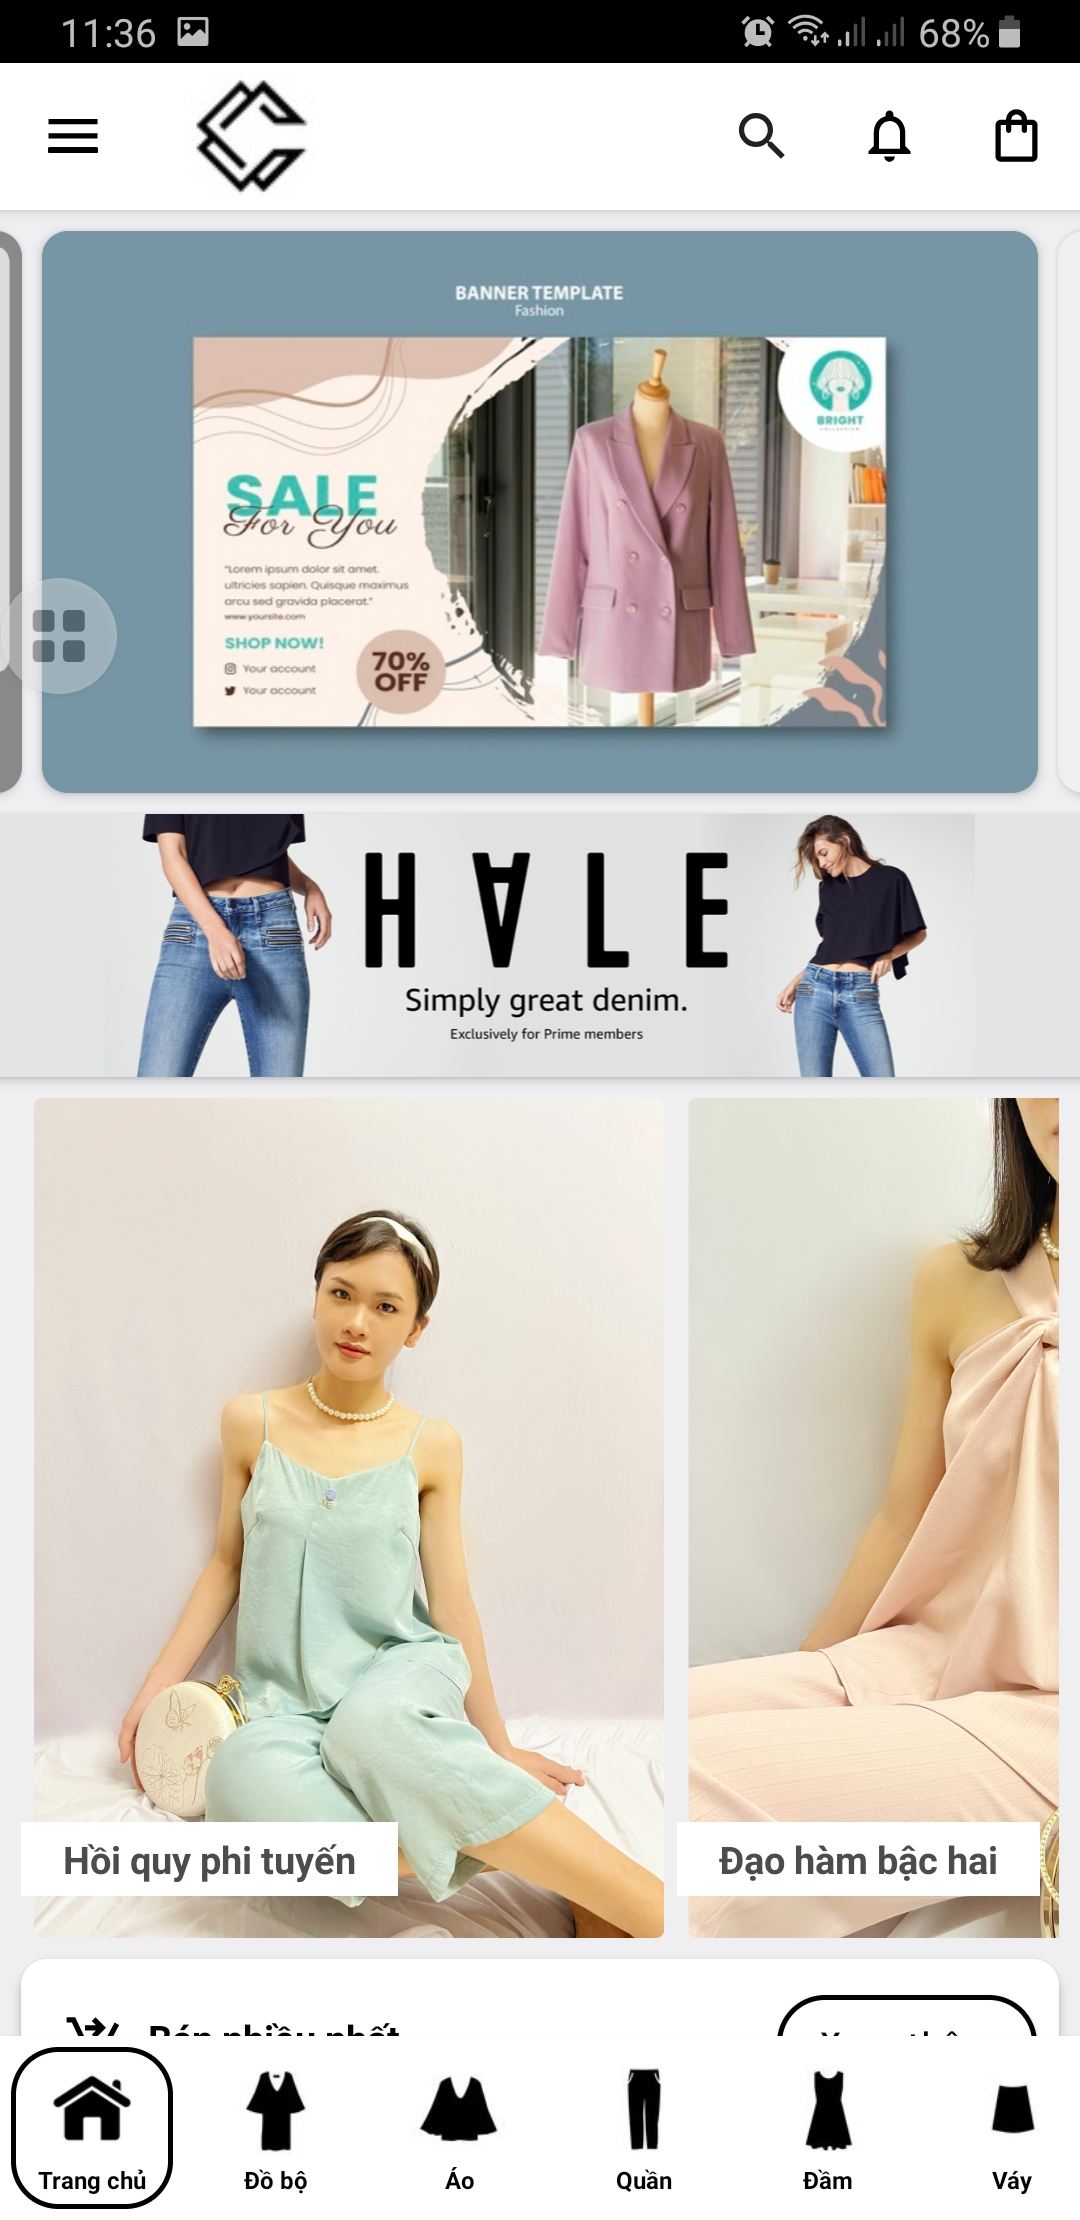
\includegraphics[height=0.7\textheight]{images/01.png}
            \caption{\centering\tiny{Hình 1: Màn hình chính của ứng dụng sau khi đăng nhập}}

        \end{figure}
        \column{0.7\linewidth}
        \begin{itemize}
            \item Clover \textbf{không phải} là một e-commerce mobile application.
            \item Clover là một \textbf{fashion mobile application} phục vụ cho các nhãn hàng thời trang mà họ không muốn kinh doanh sản phẩm của mình trên các trang thương mại điện tử.
            \item Các fashion mobile application khác mà Clover có tính năng tương tự: \href{https://play.google.com/store/apps/details?id=com.coupletx&hl=vi&gl=US}{\color{blue} CoupleTX}, \href{https://play.google.com/store/apps/details?id=vn.mrsimple&hl=en&gl=US}{\color{blue} Mr.Simple}, \href{https://play.google.com/store/apps/details?id=com.peekcloppenburg.mobileshop&hl=en&gl=US}{\color{blue} Peek \& Cloppenburg}, \href{https://play.google.com/store/apps/details?id=com.farfetch.farfetchshop&hl=en&gl=US}{\color{blue} Farfetch},...

            \item Hạn chế của ứng dụng đến hiện tại:
                  \begin{itemize}
                      \item Chưa có server.
                      \item Chưa có các web service.
                      \item Một vài chức năng còn sơ sài và chưa khớp với thực tế.
                      \item ...
                  \end{itemize}
        \end{itemize}
    \end{columns}
\end{frame}

% ============================================================================ Slide 4
\begin{frame}
    \frametitle{Các package + dịch vụ bên thứ ba (1)}
    \begin{flushleft}
        \large{\textbf{Các package:}}
        \begin{itemize}
            \item \textnormal{\href{https://github.com/vinc3m1/RoundedImageView}{\color{blue} \texttt{RoundedImageView}} - Tạo ra các \texttt{ImageView} bo tròn ở các góc, import vào gradle:}\\\texttt{\scriptsize{implementation 'com.makeramen:roundedimageview:2.3.0'}}

            \item \textnormal{\href{https://github.com/bumptech/glide}{\color{blue} \texttt{Glide}} - Load ảnh từ internet vào \texttt{ImageView}, import vào gradle:}\\\texttt{\scriptsize{implementation 'com.github.bumptech.glide:glide:4.12.0'\\annotationProcessor 'com.github.bumptech.glide:compiler:4.12.0'}}

            \item Và một vài package khác.
        \end{itemize}
    \end{flushleft}
\end{frame}

% ============================================================================ Slide 5
\begin{frame}
    \frametitle{Các package + dịch vụ bên thứ ba (2)}
    \begin{flushleft}
        \large{\textbf{Các dịch vụ bên thứ ba:}}
        \begin{itemize}
            \item \textnormal{\href{https://firebase.google.com/docs/firestore/quickstart}{\color{blue} \textsf{Firebase Firestore}} - CSDL NoSQL do Google phát triển.}

            \item \textnormal{Firebase FireStorage - Dùng để lưu trữ tệp tin, thư mục trên cloud, nhóm không tìm thấy document do Google công bố cho dịch vụ này, nhưng để sử dụng thì nhóm tìm hiểu trong cuốn} \href{https://www.amazon.com/Mastering-Firebase-Android-Development-cloud-enabled/dp/1788624718}{\color{teal} Mastering Firebase for Android Development}.

            \item \textnormal{\href{https://firebase.google.com/docs/auth/android/start}{\color{blue} \textsf{Firebase Authentication}} - Dịch vụ xác nhận danh tính, đăng ký tài khoản người dùng do Google phát triển.}
        \end{itemize}
    \end{flushleft}
\end{frame}

% ============================================================================ Slide 6
\begin{frame}
    \frametitle{Các màn hình và chức năng kèm theo (1)}
    \framesubtitle{Nội dung}
    \begin{flushleft}
        \large{\textbf{Các màn hình chính và chức năng quan trọng được trình bày:}}
        \begin{enumerate}
            \item Màn hình đăng nhập.
            \item Màn hình chi tiết sản phẩm.
            \item Màn hình chính.
            \item Chức năng tìm kiếm.
        \end{enumerate}
    \end{flushleft}

    \begin{flushleft}
        \begin{block}{}
            Ngoài ra còn có các màn hình khác như \textsf{\color{teal} Giỏ hàng, Lịch sử mua hàng, Tài khoản người dùng,...} nhưng đơn giản và đa phần được kế thừa từ các màn hình trên nên nhóm xin rút gọn phần trình bày cho chúng.
        \end{block}
    \end{flushleft}
\end{frame}

% ============================================================================ Slide 7
\begin{frame}
    \frametitle{Các màn hình và chức năng kèm theo (2)}
    \framesubtitle{Màn hình đăng nhập}

    \begin{columns}
        \column{0.3\linewidth}
        \begin{figure}
            \centering
            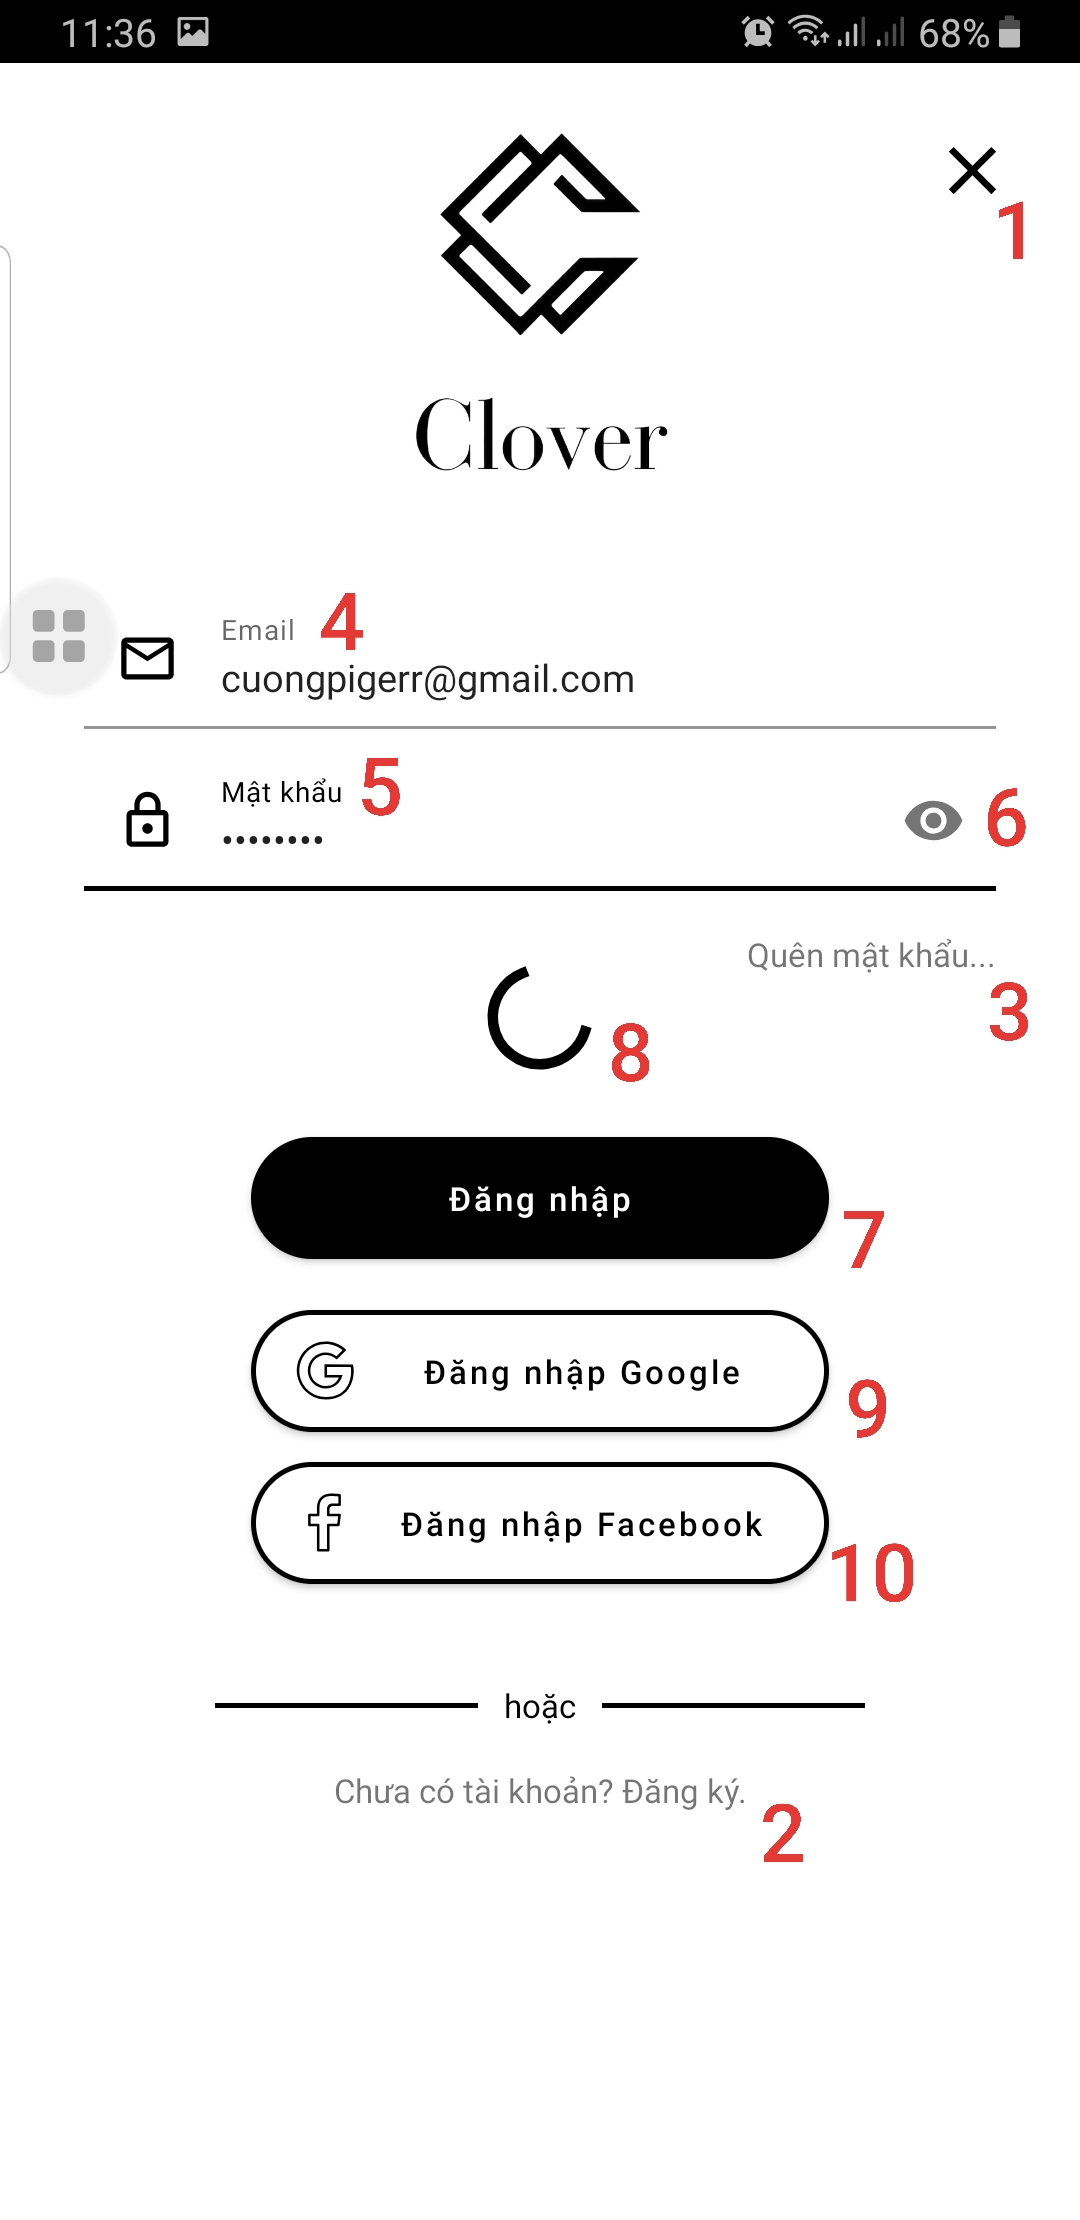
\includegraphics[height=0.7\textheight]{images/02.png}
            \caption{\centering\tiny{Hình 2: Màn hình đăng nhập}}

        \end{figure}
        \column{0.7\linewidth}
        \indent \textbf{Các thành phần và chức năng kèm theo trên màn hình:}
        \begin{itemize}
            \item \textbf{1}: Image button - khi nhấn vào button này người dùng sẽ được chuyển thẳng đến màn hình chính của ứng dụng mà \textbf{không cần đăng nhập}.
            \item \textbf{2}: Text button - khi nhấn vào sẽ đưa đến fragment đăng ký tài khoản mới cho người dùng.
            \item \textbf{3}: Text button - khi nhấn vào đưa người dùng đến fragment đặt lại mật khẩu.
            \item \textbf{4}: Text input layout - nhập thông tin email của người dùng.
        \end{itemize}
    \end{columns}
\end{frame}

% ============================================================================ Slide 8
\begin{frame}
    \begin{columns}
        \column{0.3\linewidth}
        \begin{figure}
            \centering
            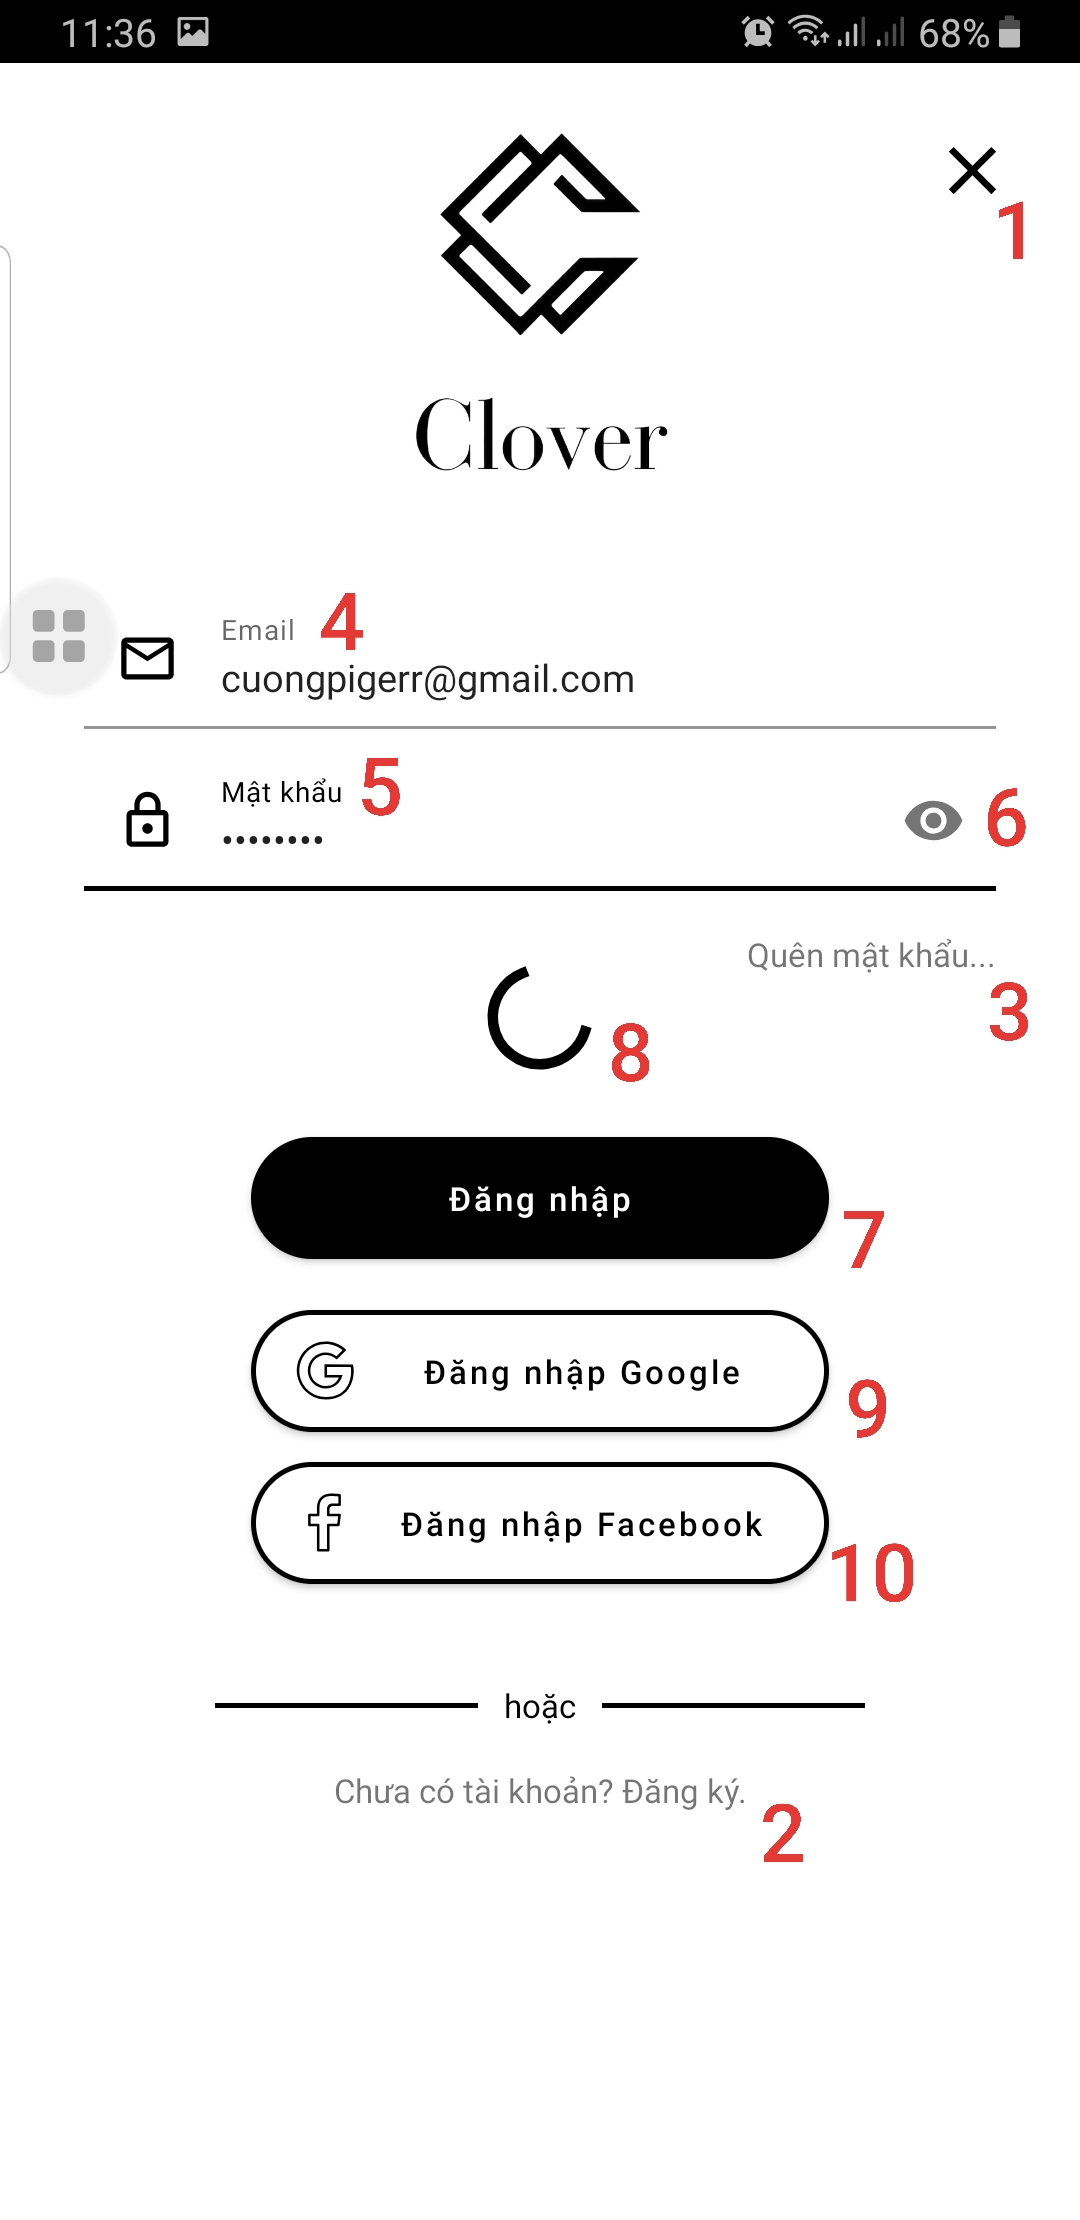
\includegraphics[height=0.7\textheight]{images/02.png}
            \caption{\centering\tiny{Hình 2: Màn hình đăng nhập}}

        \end{figure}
        \column{0.7\linewidth}
        \indent \textbf{Các thành phần và chức năng kèm theo trên màn hình:}
        \begin{itemize}
            \item \textbf{5}: Text input layout - nhập mật khẩu của người dùng.
            \item \textbf{6}: Icon - khi nhấn vào sẽ hiển thị mật khẩu ở \textbf{5} ra dưới dạng text.
            \item \textbf{7}: Button - nhấn vào để đăng nhập.
            \item \textbf{8}: Progress Circle - luôn ẩn đi, chỉ hiển thị khi người dùng nhấn vào \textbf{7} để cho người dùng biết rằng hệ thống vẫn chạy và đang trong quá trình kiểm tra đăng nhập.
        \end{itemize}
    \end{columns}
\end{frame}


\begin{frame}
    \frametitle{Các màn hình và chức năng kèm theo (3)}
    \framesubtitle{Màn hình đăng nhập - Mã nguồn minh họa}

    \begin{columns}
        \column{0.3\linewidth}
        \begin{figure}
            \centering
            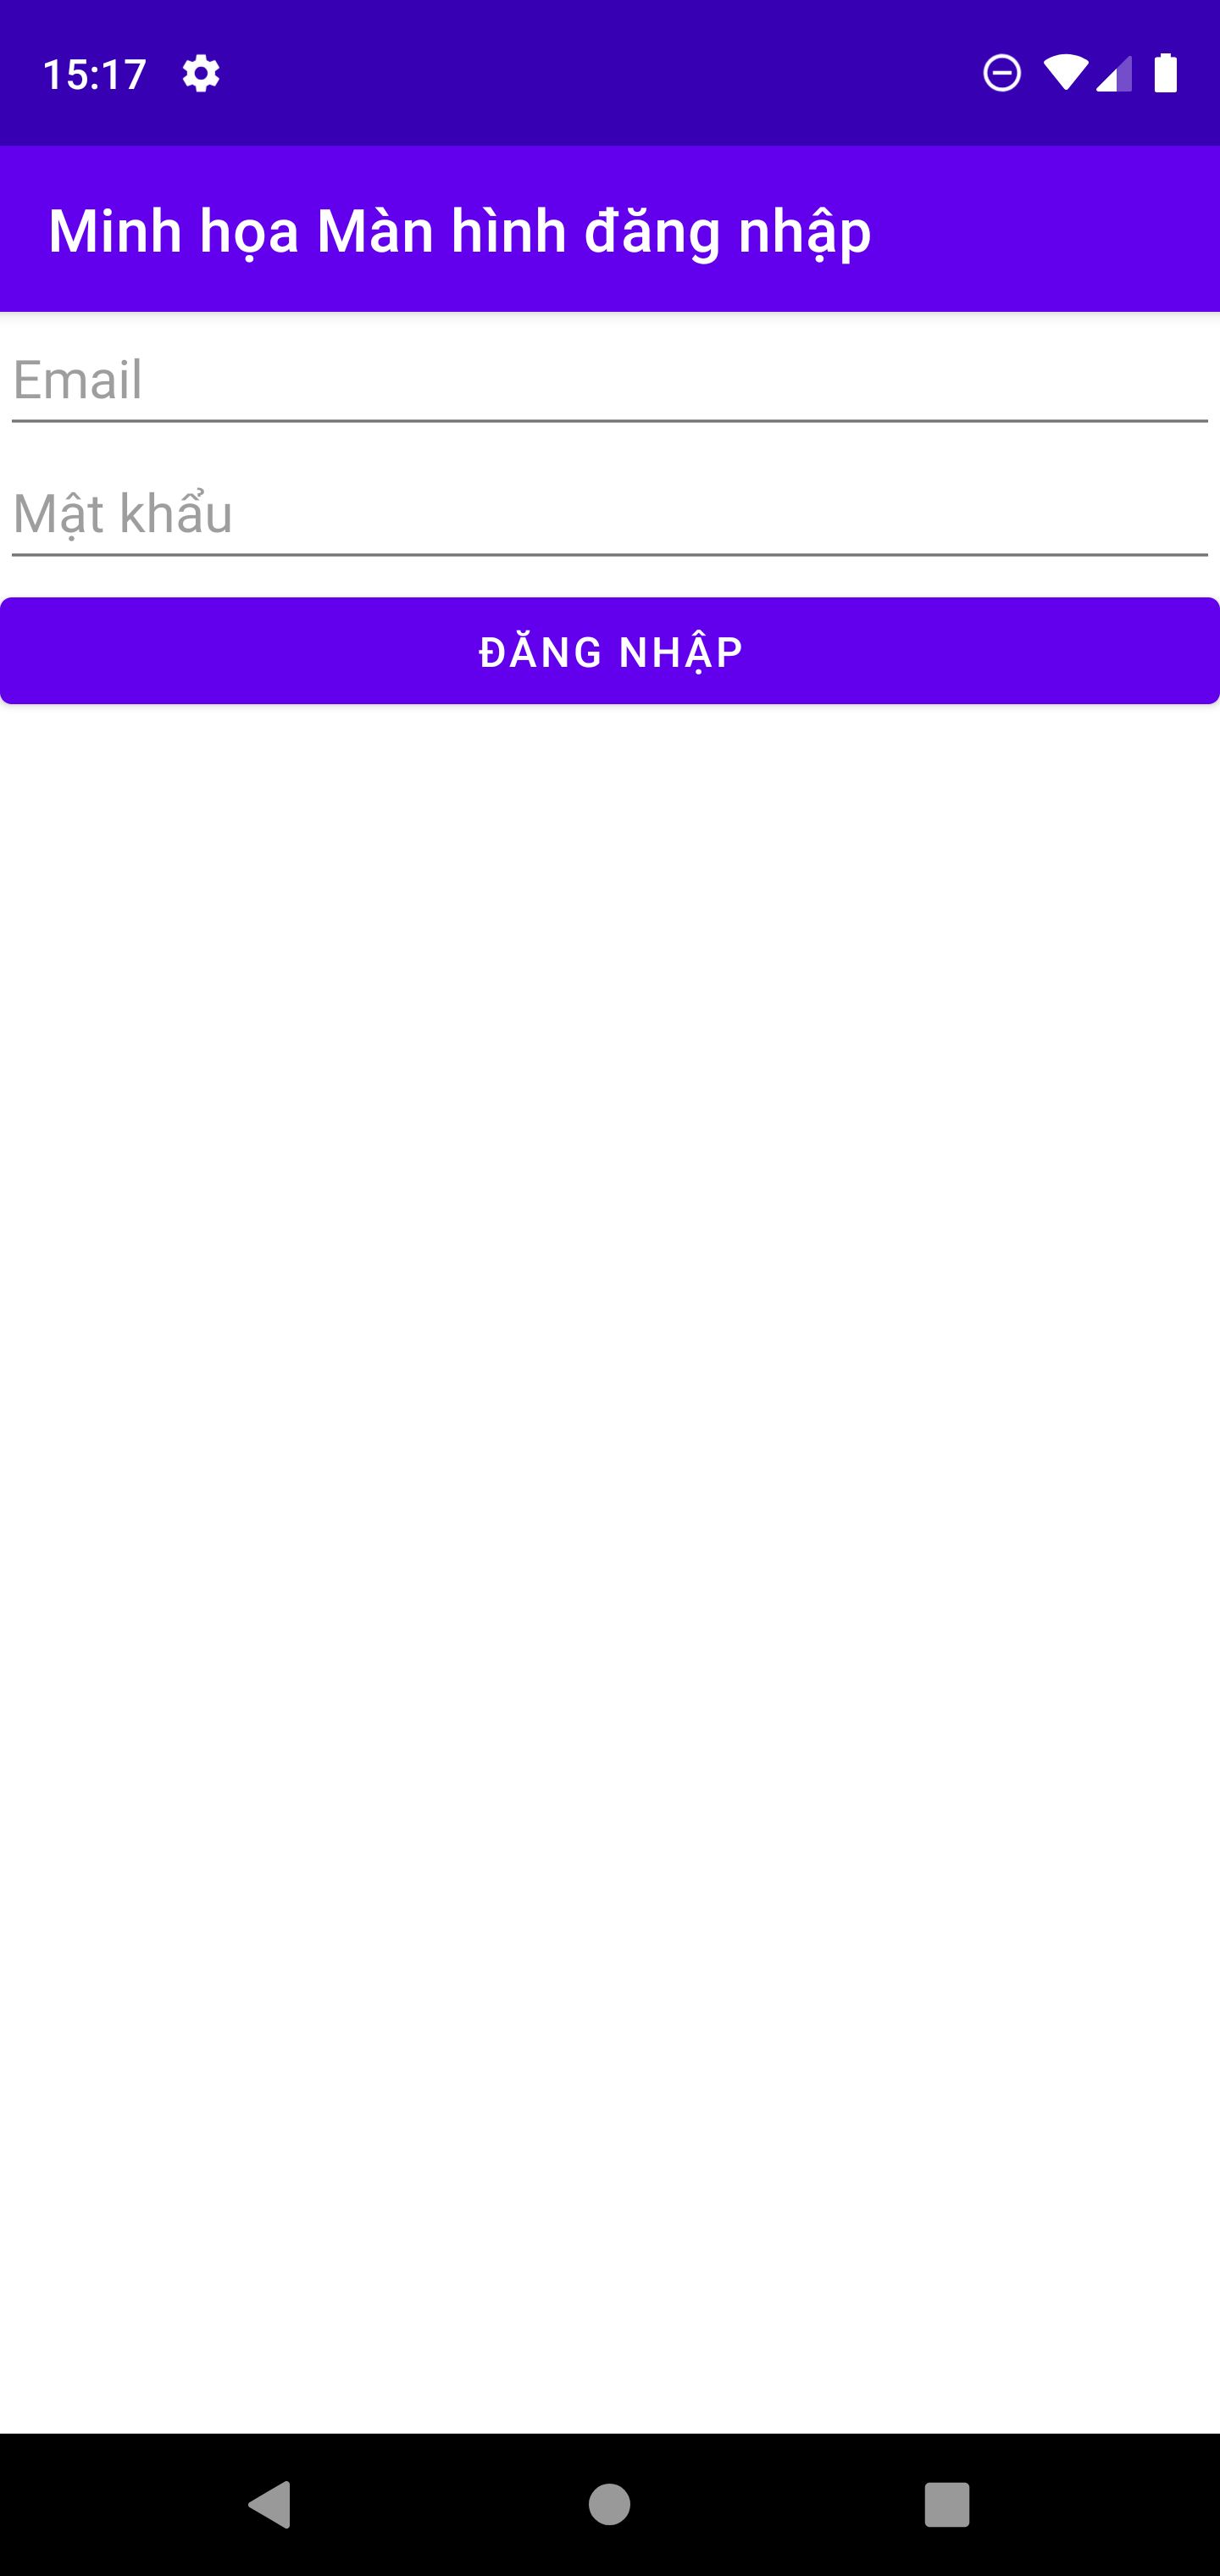
\includegraphics[height=0.7\textheight]{images/24.png}
            \caption{\centering\tiny{Hình 3: Minh họa màn hình đăng nhập}}
        \end{figure}
        \column{0.7\linewidth}
        \indent Cấu trúc cây thư mục:
        \begin{figure}
            \centering
            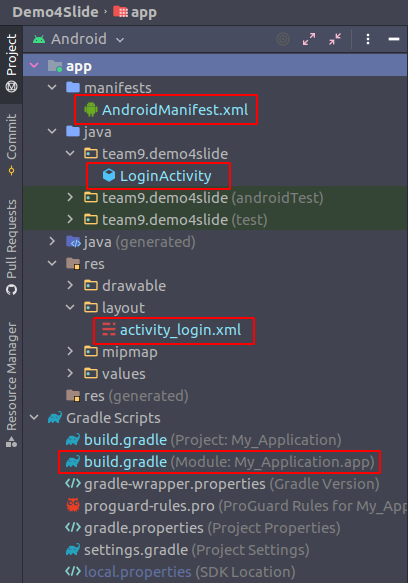
\includegraphics[height=0.68\textheight]{images/25.png}
        \end{figure}
    \end{columns}
\end{frame}

\begin{frame}
    \begin{columns}
        \column{0.3\linewidth}
        \begin{figure}
            \centering
            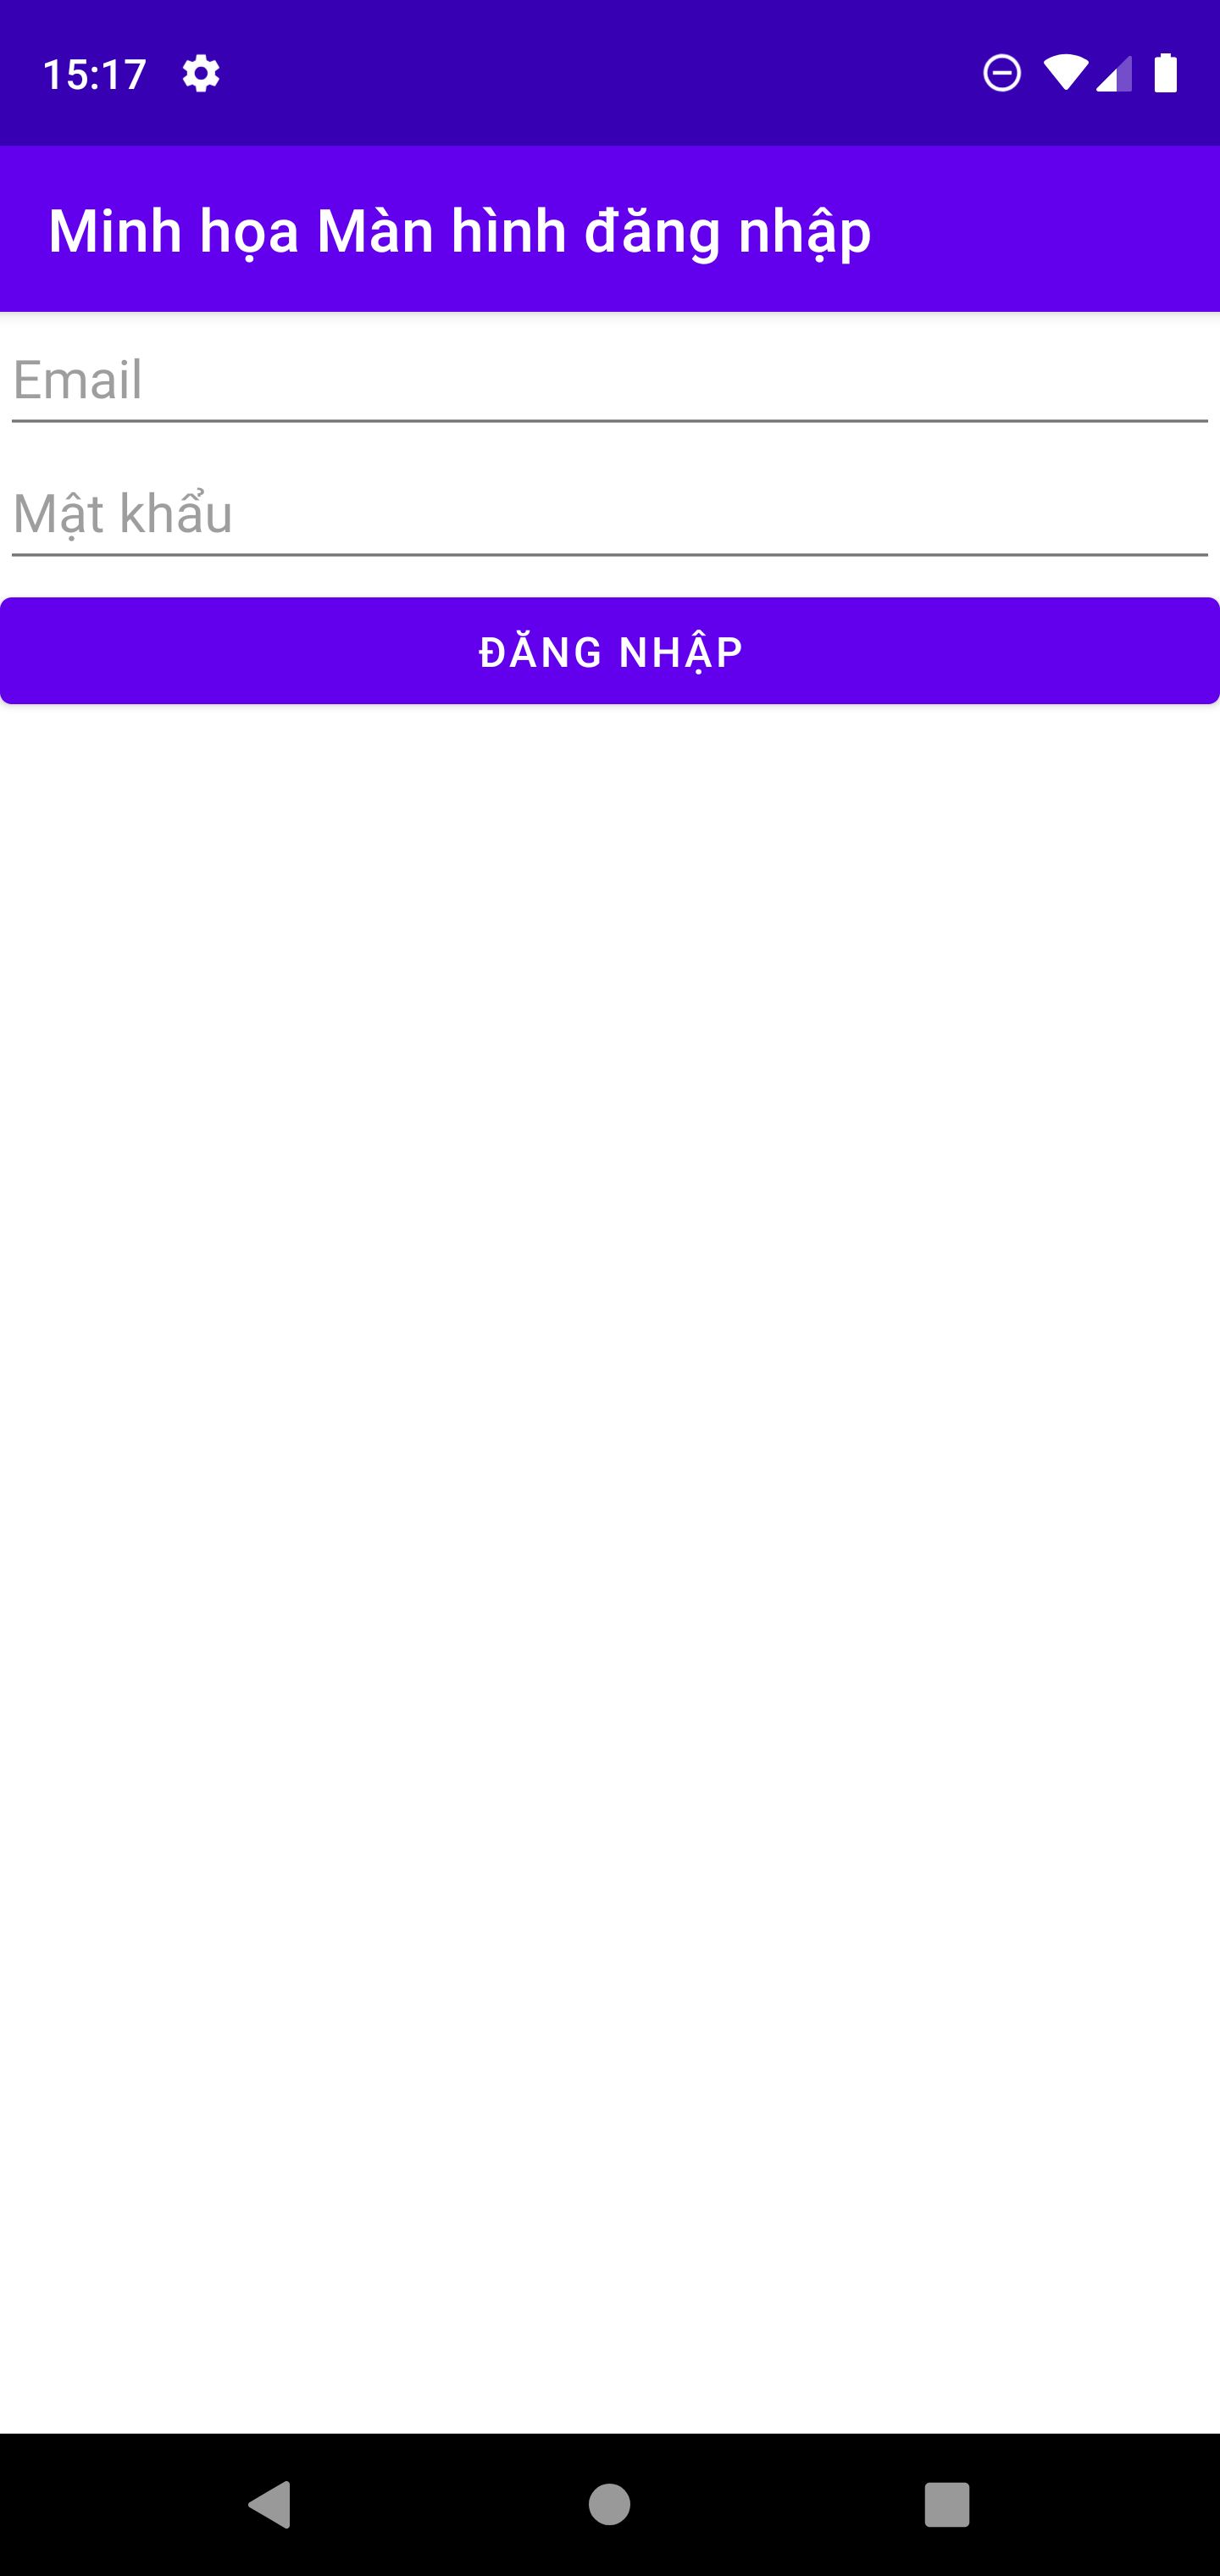
\includegraphics[height=0.7\textheight]{images/24.png}
            \caption{\centering\tiny{Hình 3: Minh họa màn hình đăng nhập}}
        \end{figure}
        \column{0.7\linewidth}
        \indent \texttt{AndroidManifest.xml}
        \begin{figure}
            \centering
            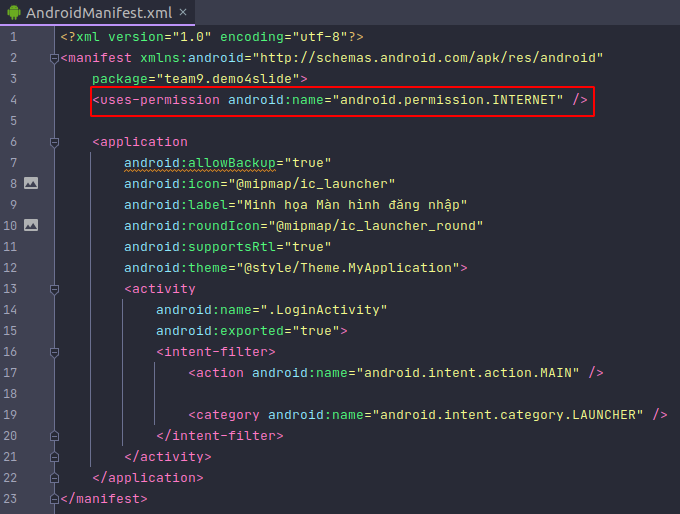
\includegraphics[width=\textwidth]{images/26.png}
        \end{figure}
    \end{columns}
\end{frame}


\begin{frame}
    \begin{columns}
        \column{0.3\linewidth}
        \begin{figure}
            \centering
            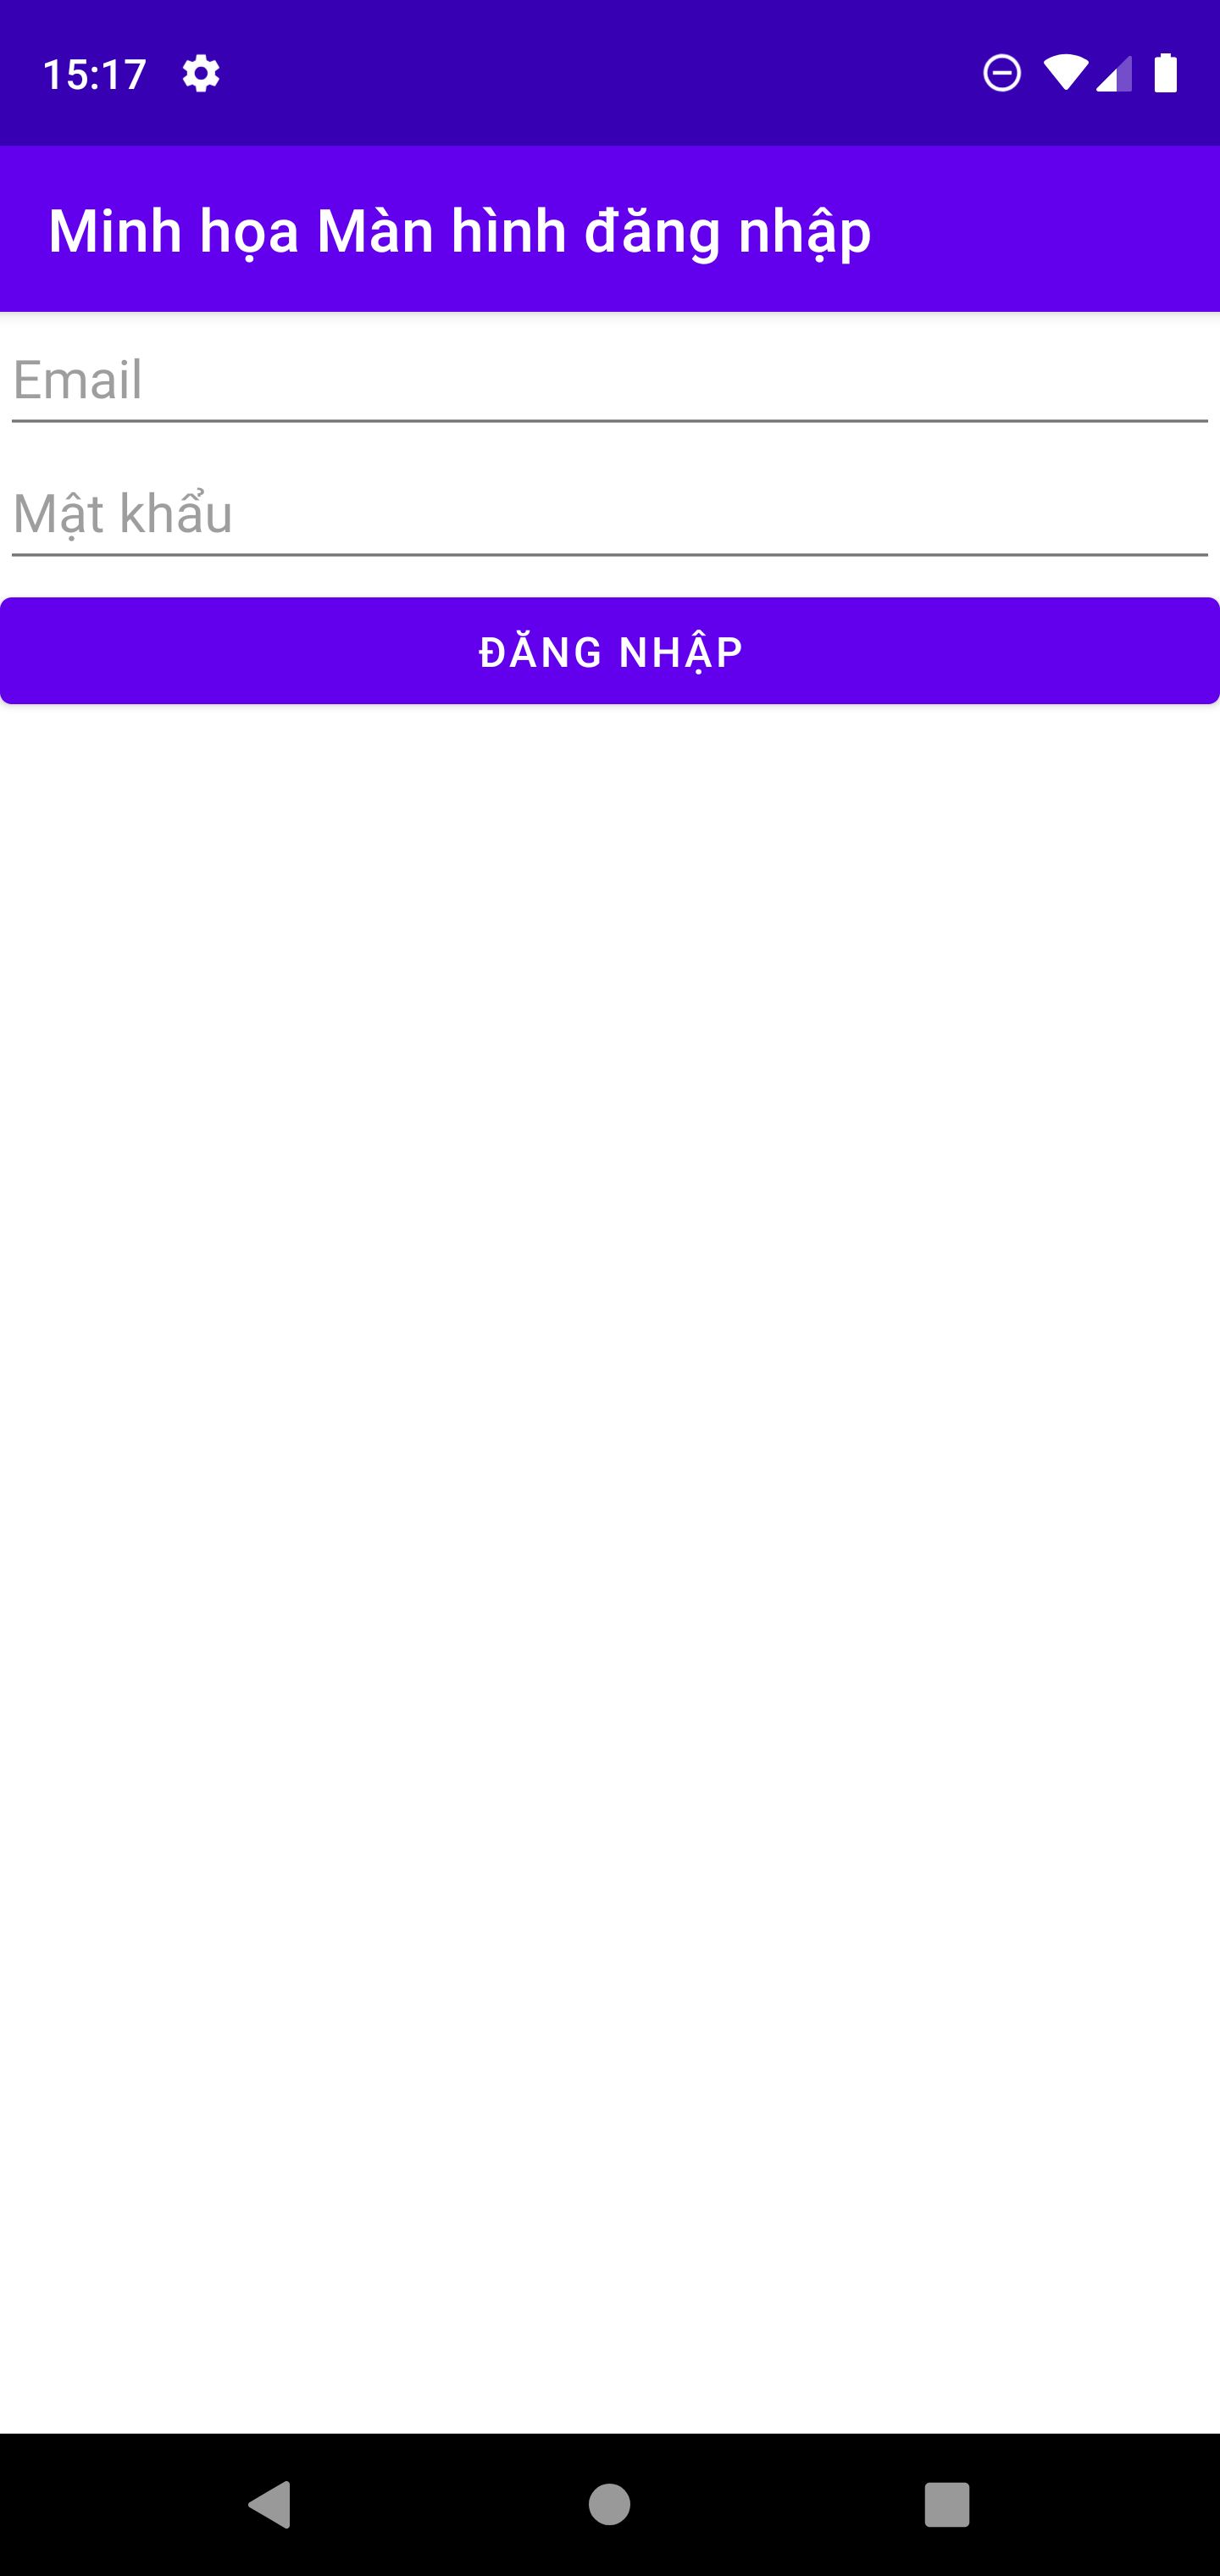
\includegraphics[height=0.7\textheight]{images/24.png}
            \caption{\centering\tiny{Hình 3: Minh họa màn hình đăng nhập}}
        \end{figure}
        \column{0.7\linewidth}
        \indent \texttt{build.gradle}
        \begin{figure}
            \centering
            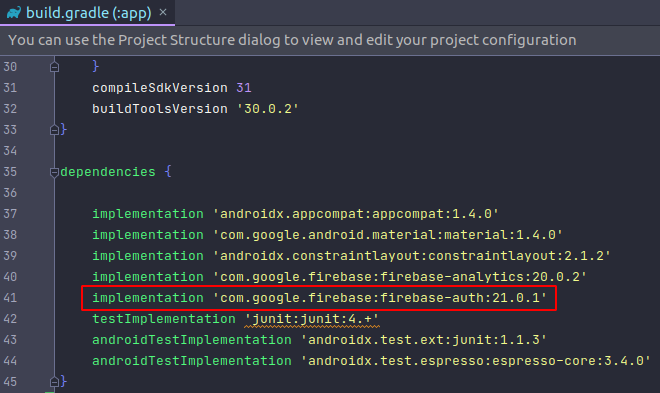
\includegraphics[width=\textwidth]{images/27.png}
        \end{figure}
    \end{columns}
\end{frame}

\begin{frame}
    \begin{columns}
        \column{0.3\linewidth}
        \begin{figure}
            \centering
            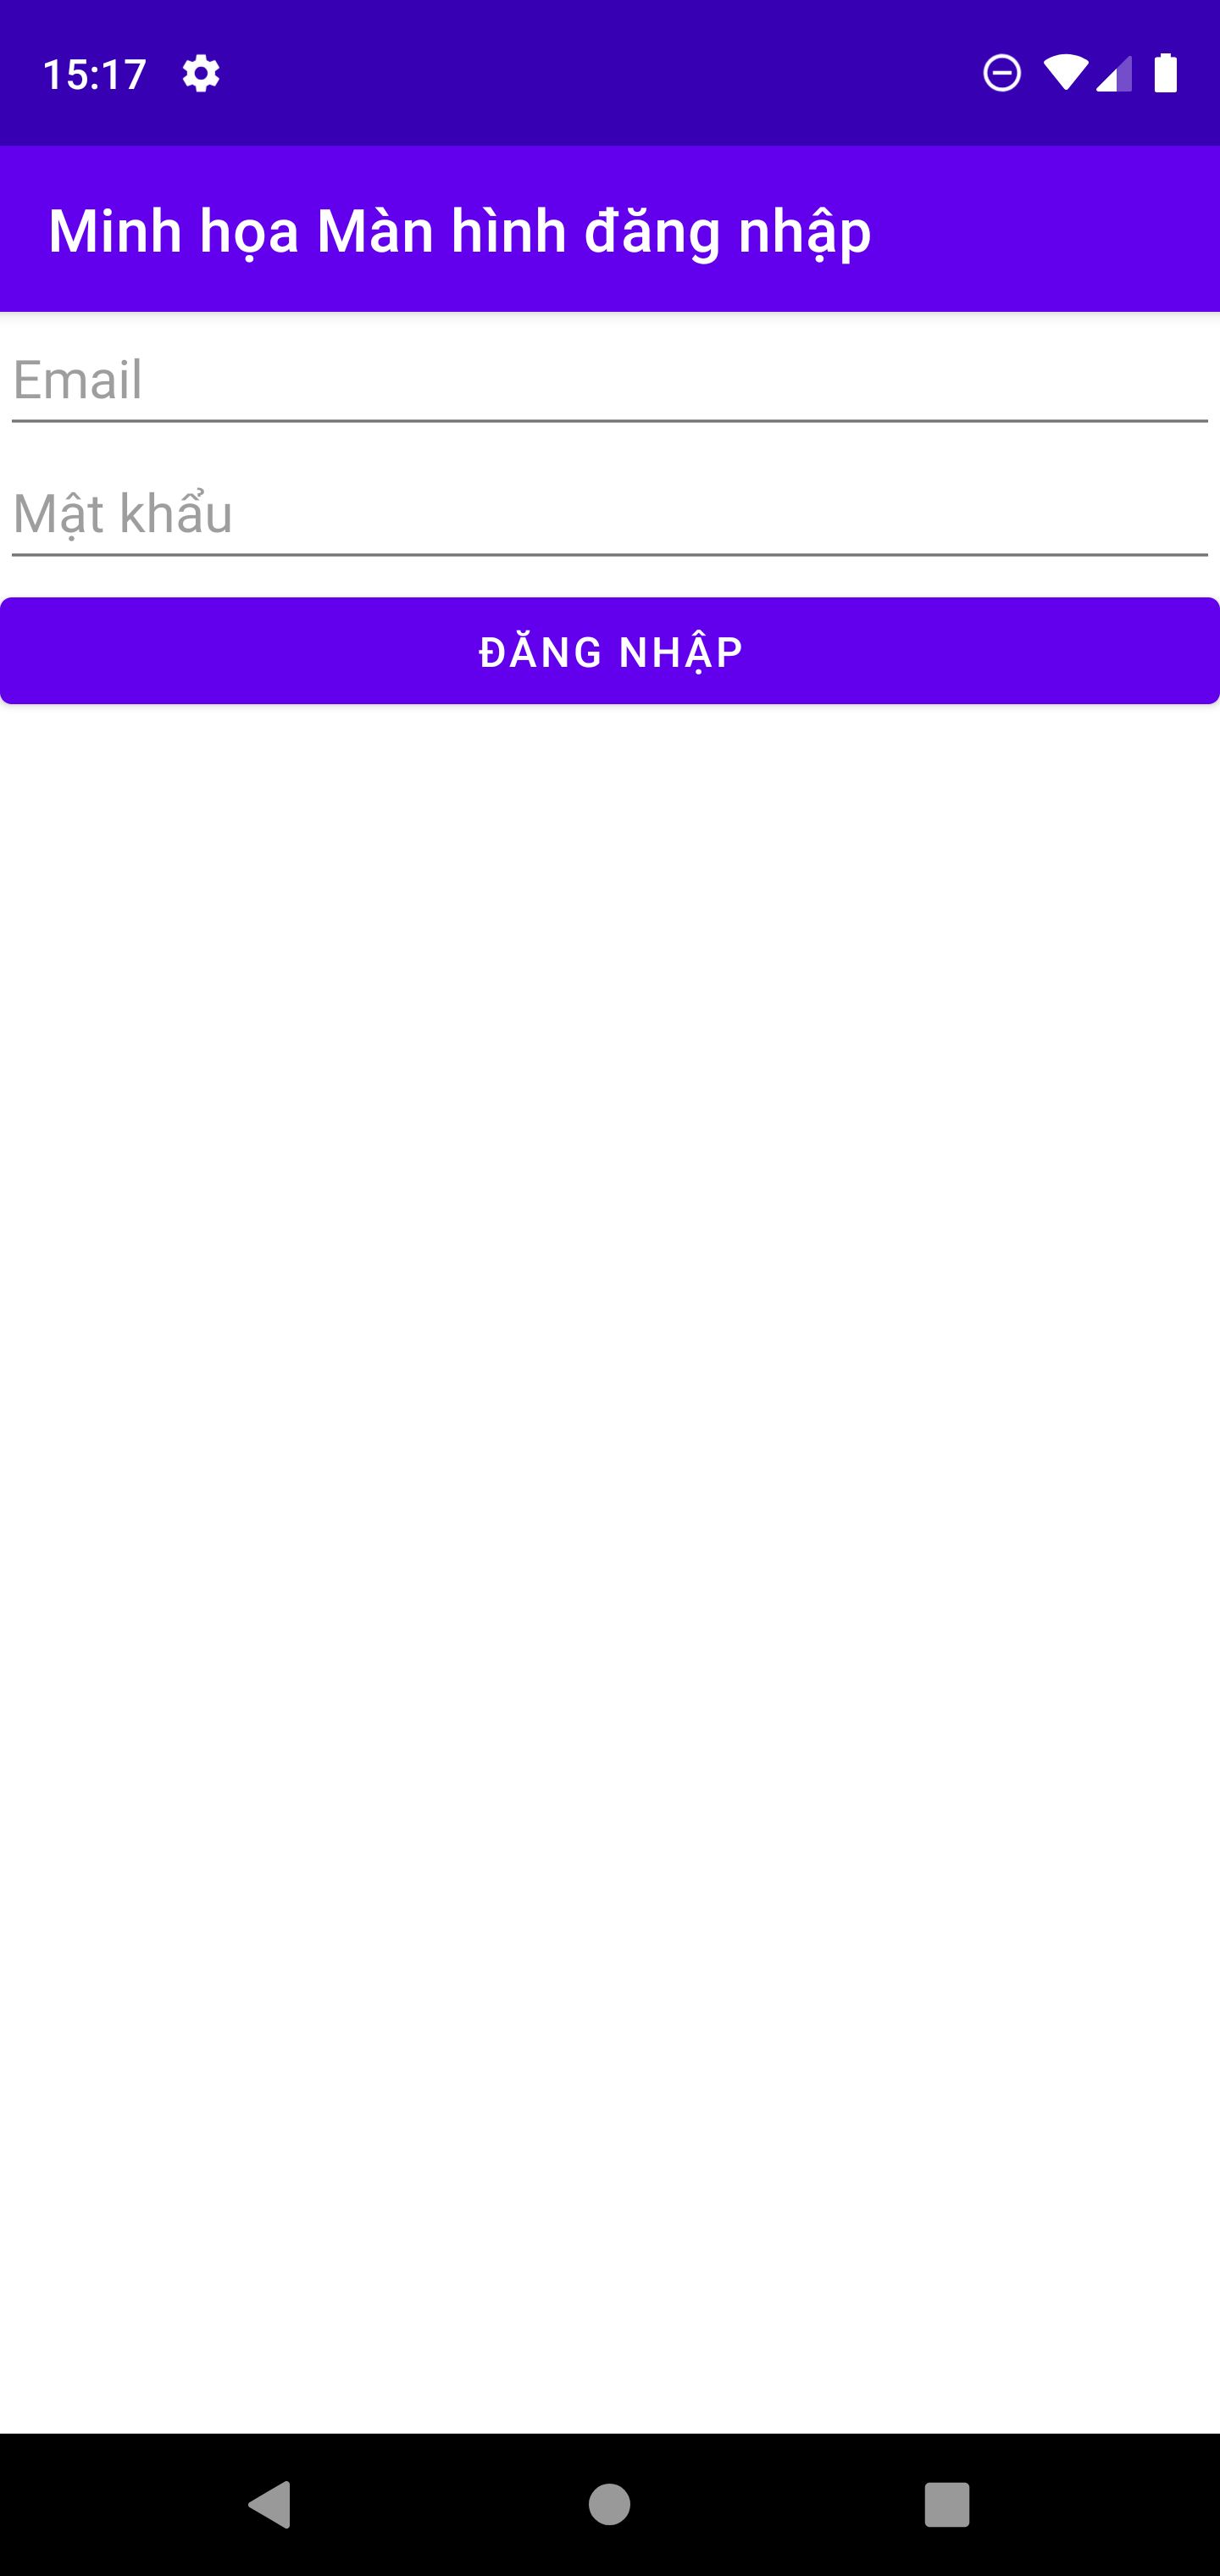
\includegraphics[height=0.7\textheight]{images/24.png}
            \caption{\centering\tiny{Hình 3: Minh họa màn hình đăng nhập}}
        \end{figure}
        \column{0.7\linewidth}
        \indent \texttt{activity\_login.xml}
        \begin{figure}
            \centering
            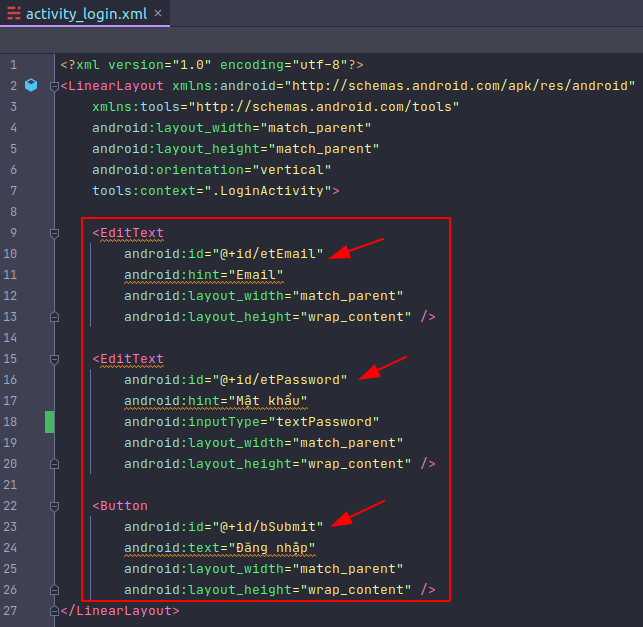
\includegraphics[width=\textwidth]{images/28.png}
        \end{figure}
    \end{columns}
\end{frame}


\begin{frame}
    \begin{columns}
        \column{0.3\linewidth}
        \begin{figure}
            \centering
            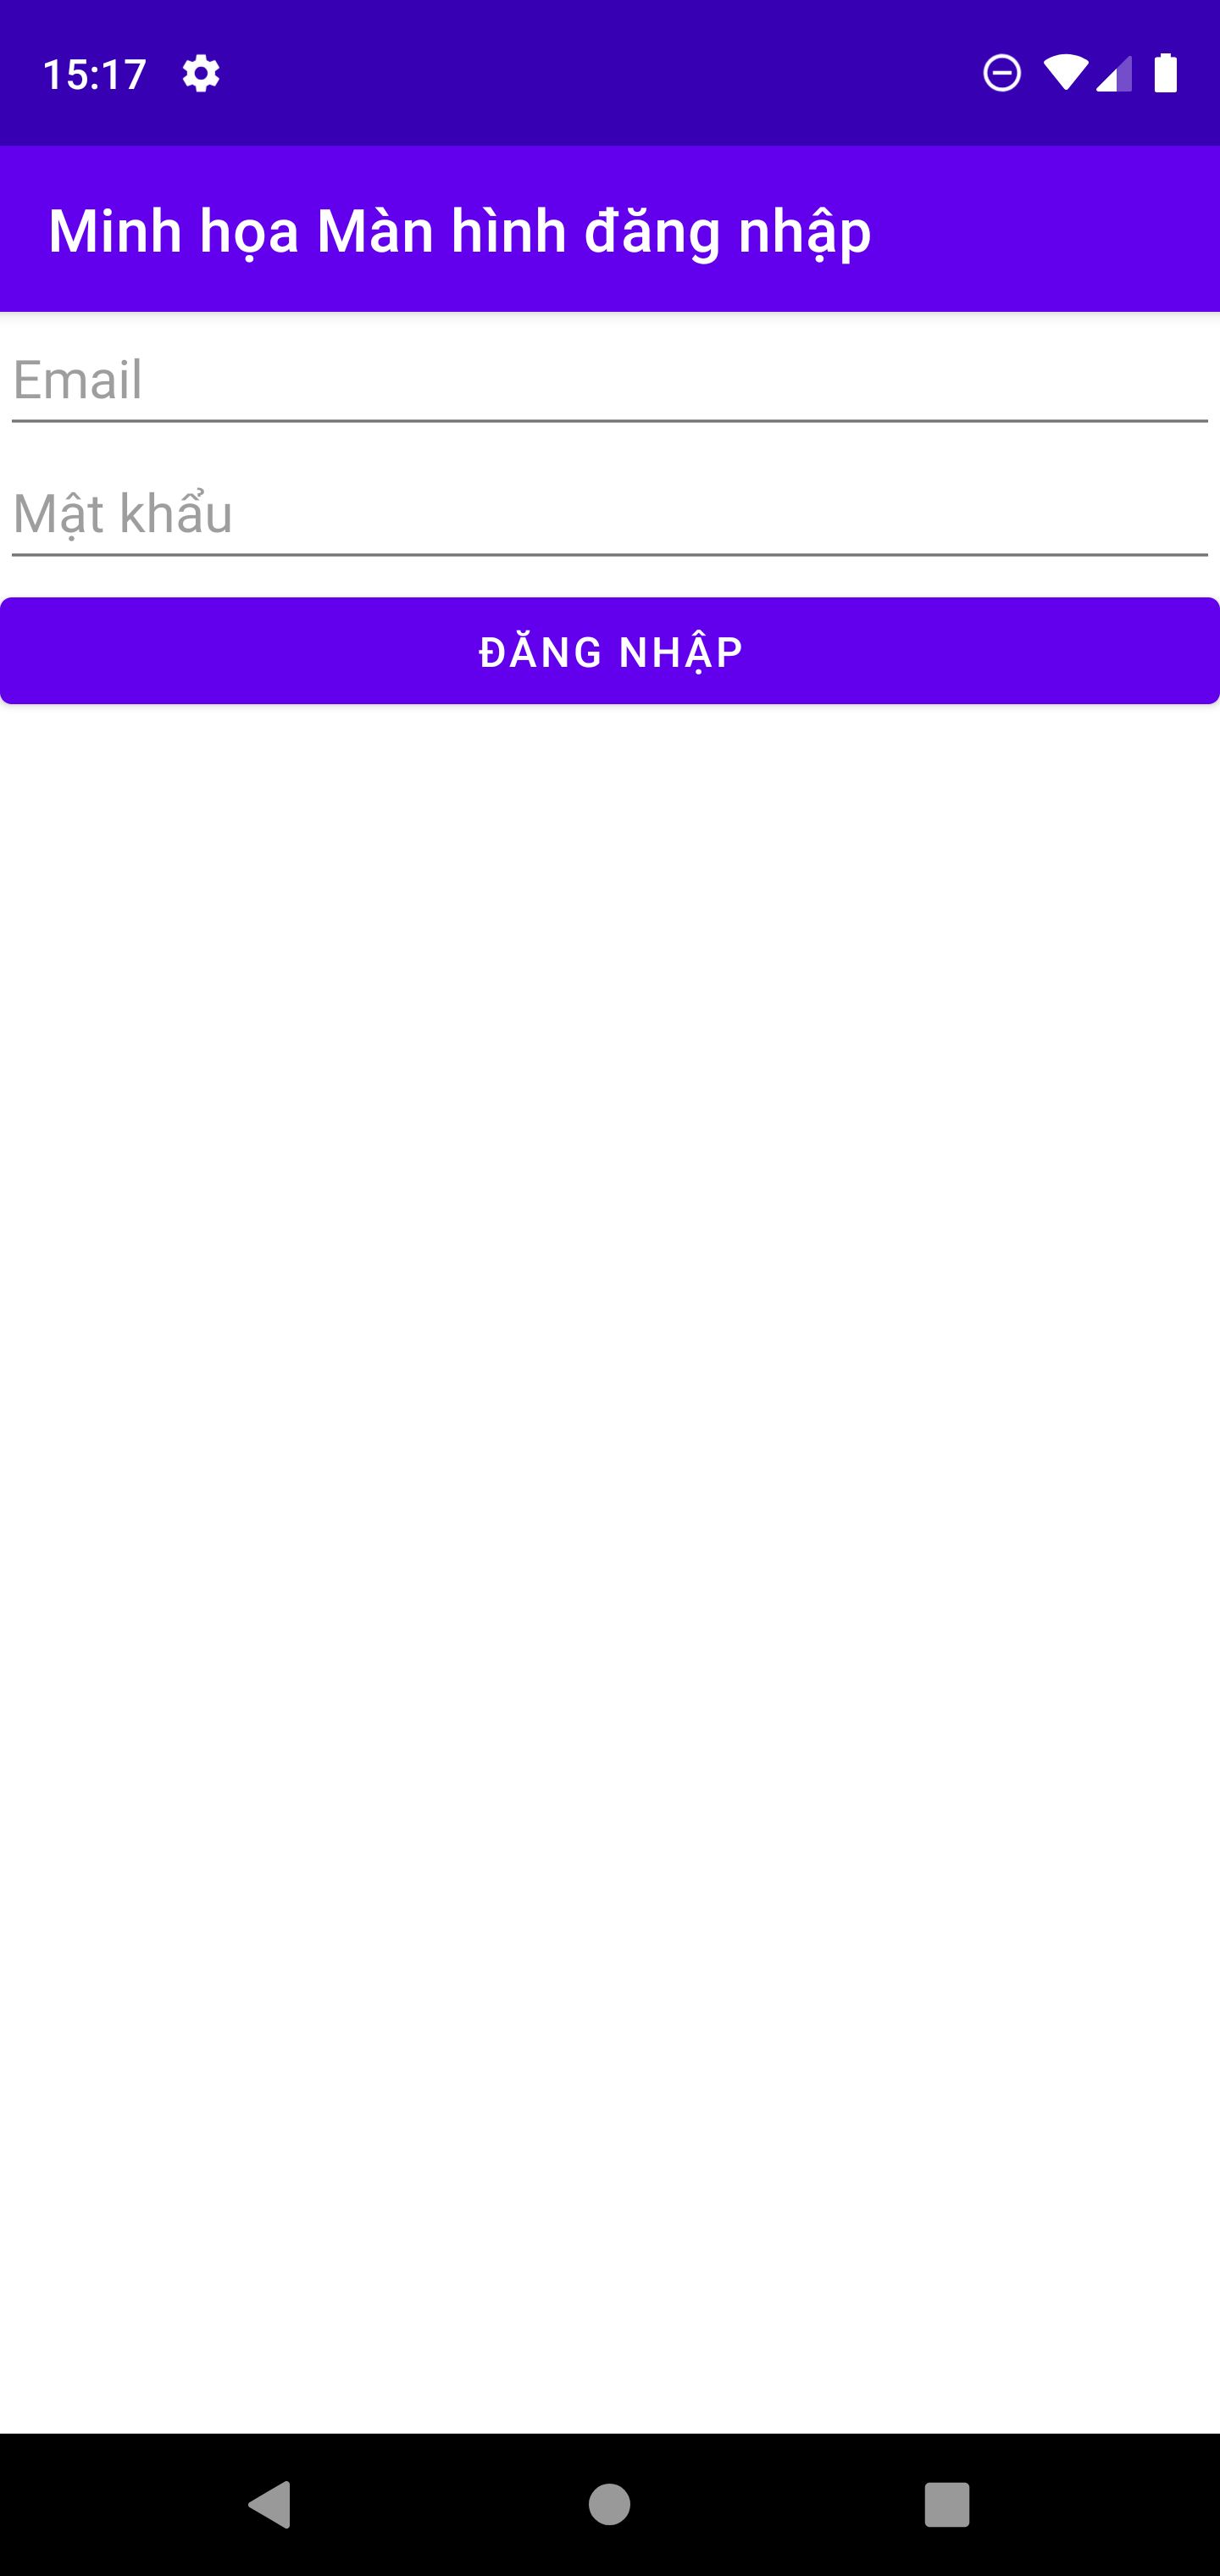
\includegraphics[height=0.7\textheight]{images/24.png}
            \caption{\centering\tiny{Hình 3: Minh họa màn hình đăng nhập}}
        \end{figure}
        \column{0.7\linewidth}
        \indent \texttt{LoginActivity.java}
        \begin{figure}
            \centering
            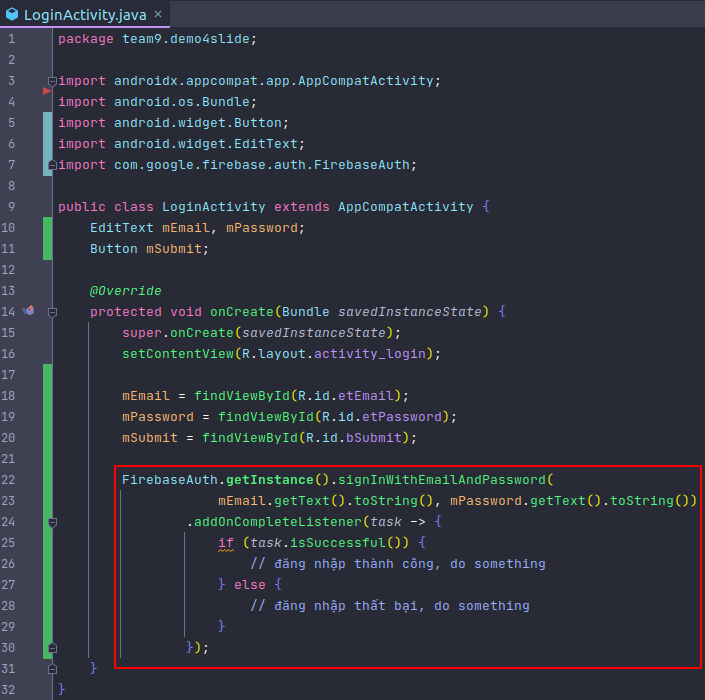
\includegraphics[width=\textwidth]{images/29.png}
        \end{figure}
    \end{columns}
\end{frame}

% ============================================================================ Slide 9
\begin{frame}
    \frametitle{Các màn hình và chức năng kèm theo (4)}
    \framesubtitle{Màn hình chi tiết sản phẩm}

    \begin{columns}
        \column{0.3\linewidth}
        \begin{figure}
            \centering
            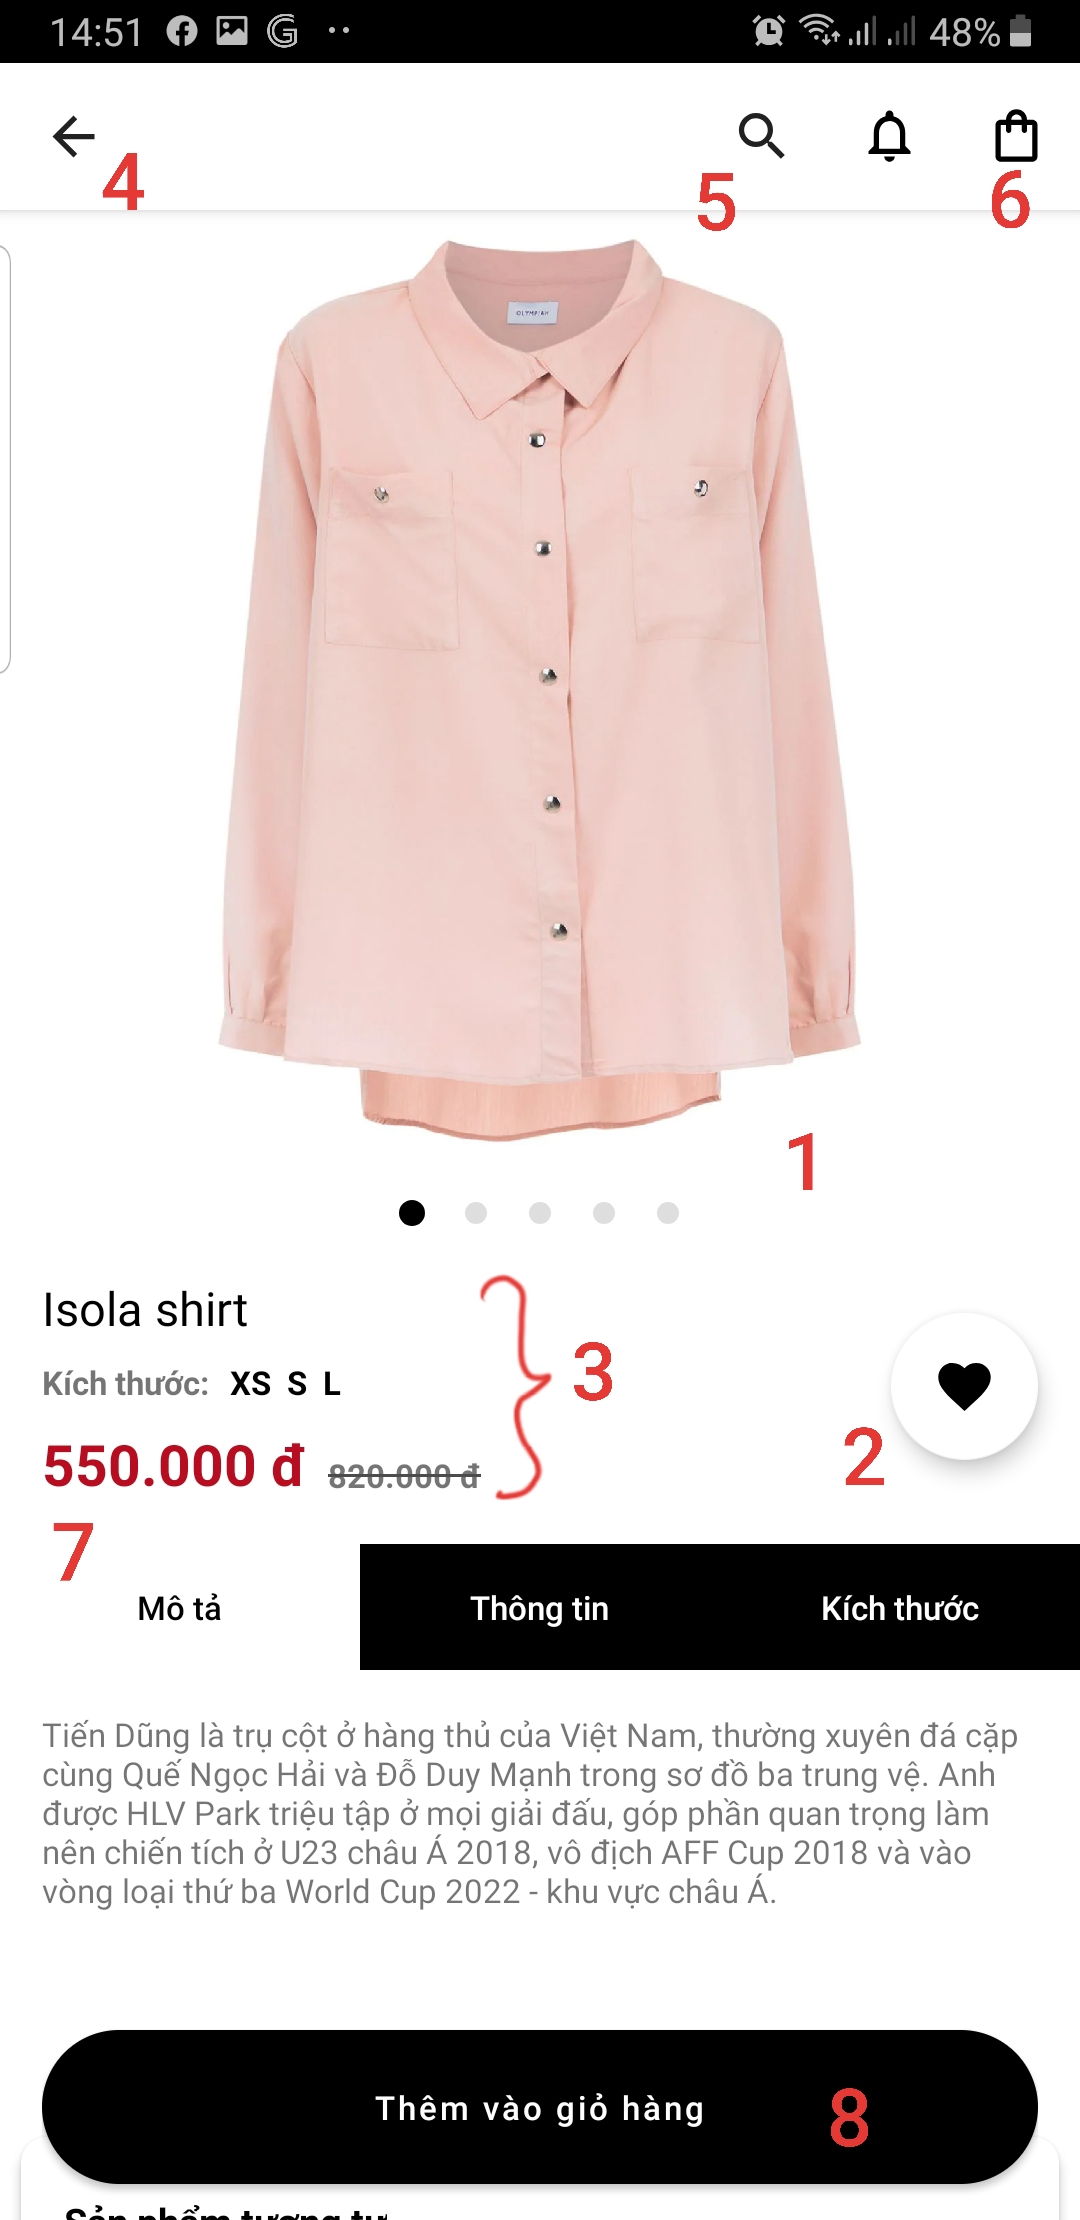
\includegraphics[height=0.7\textheight]{images/03.png}
            \caption{\centering\tiny{Hình 4: Màn hình chi tiết sản phẩm 1}}

        \end{figure}
        \column{0.7\linewidth}
        \indent \textbf{Các thành phần và chức năng kèm theo trên màn hình:}
        \begin{itemize}
            \item \textbf{1}: View Pager - hiển thị các hình ảnh của sản phẩm.
            \item \textbf{2}: Floating Action Button - cho phép người dùng nhấn vào để thêm sản phầm vào mục yêu thích.
            \item \textbf{3}: Các text view - hiển thị thông tin của sản phẩm.
            \item \textbf{4}: As home indicator - quay về fragment trước đó được lưu trong backstack.
        \end{itemize}
    \end{columns}
\end{frame}

% =========================================================================== Slide 10
\begin{frame}
    \begin{columns}
        \column{0.3\linewidth}
        \begin{figure}
            \centering
            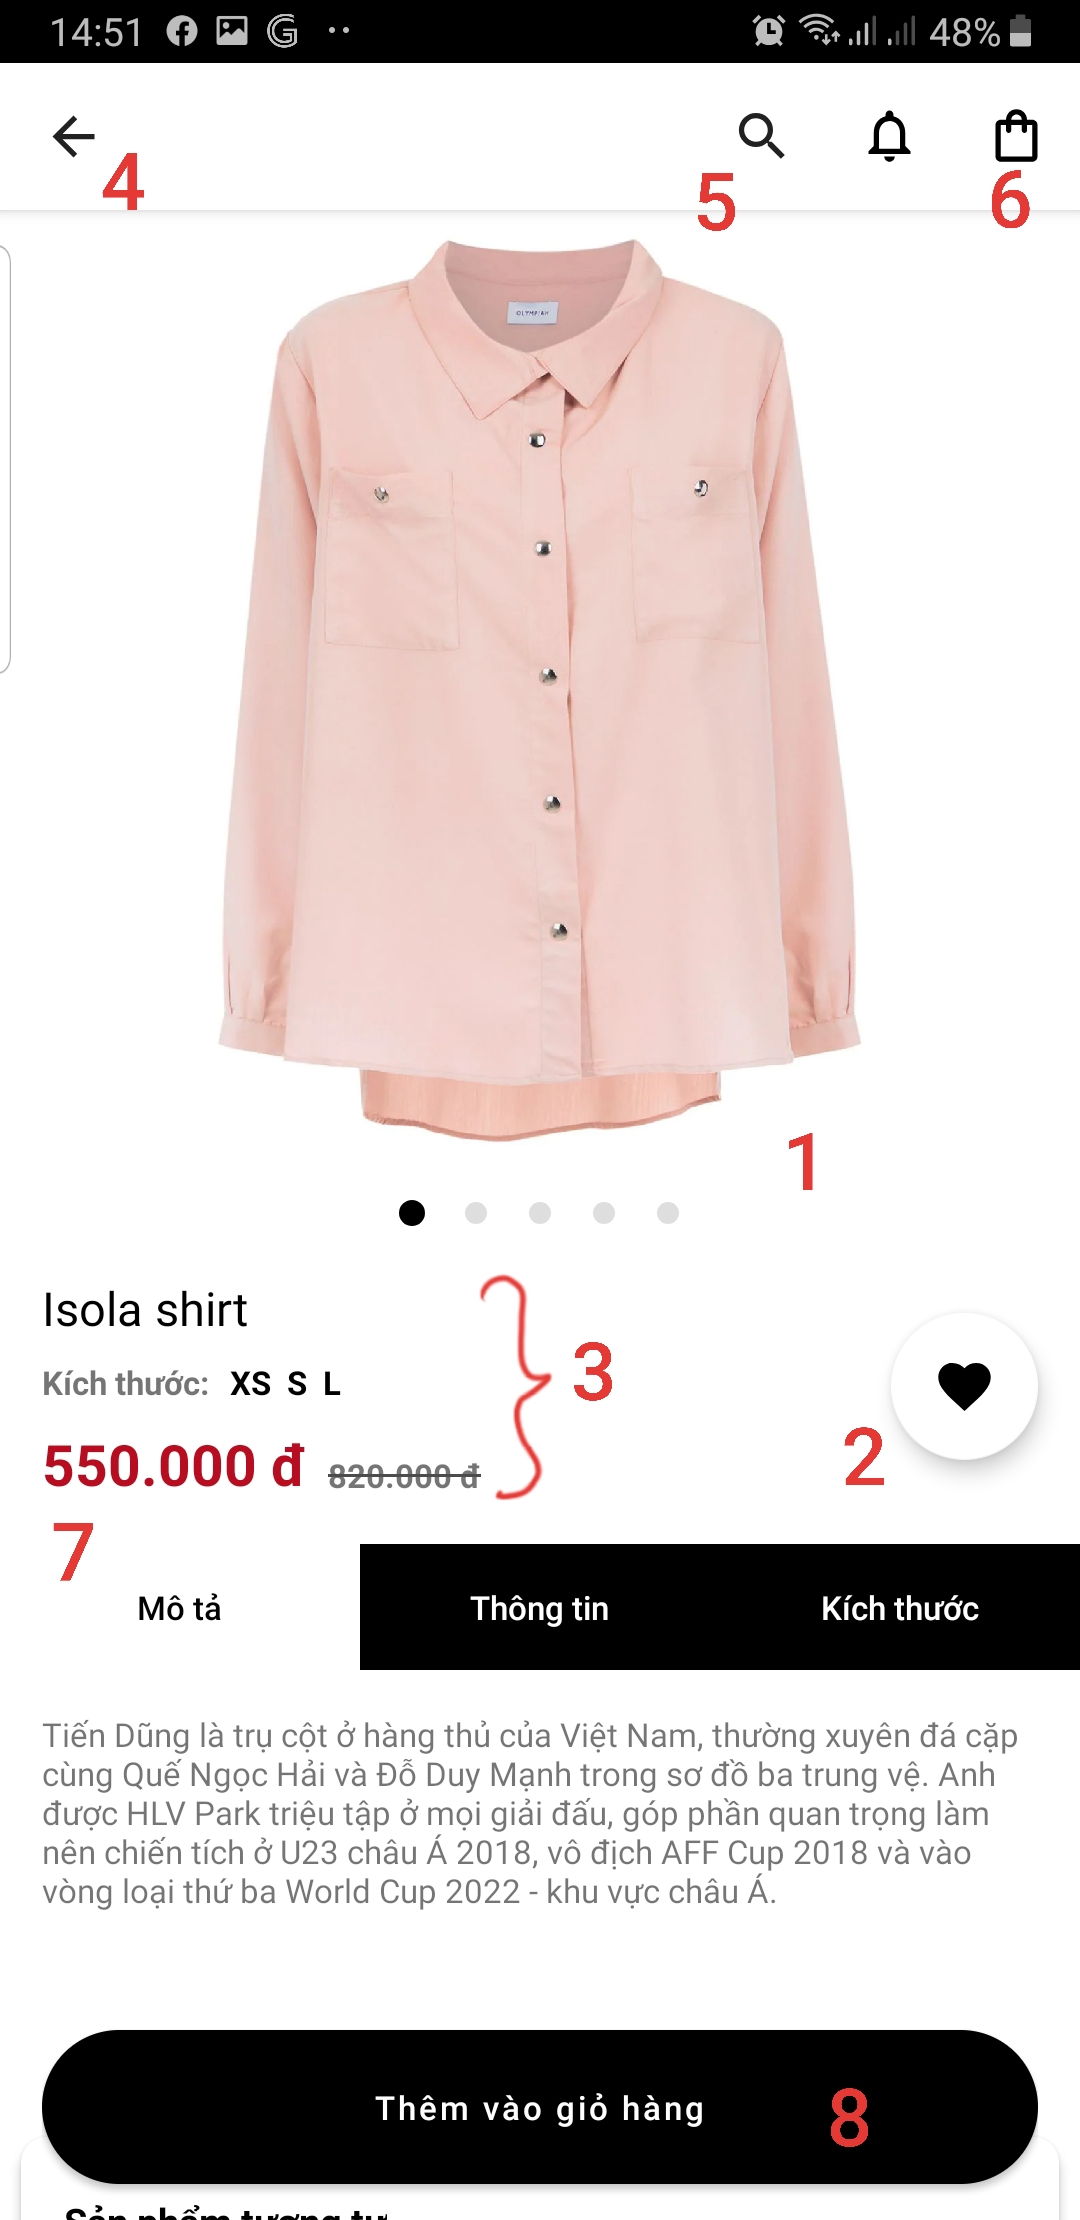
\includegraphics[height=0.7\textheight]{images/03.png}
            \caption{\centering\tiny{Hình 4: Màn hình chi tiết sản phẩm 1}}

        \end{figure}
        \column{0.7\linewidth}
        \indent \textbf{Các thành phần và chức năng kèm theo trên màn hình:}
        \begin{itemize}
            \item \textbf{5}: Menu item Search - nhấn vào để thực hiện chức năng tìm kiếm.
            \item \textbf{6}: Menu item Cart - nhấn vào để đến fragment giỏ hàng.
            \item \textbf{7}: TabLayout + View Pager 2 - bên trong tab "Mô tả" là một Text View.
            \item \textbf{8}: Button - nhấn vào sẽ hiện một Dialog để người dùng có thể chọn size và số lượng sản phẩm để thêm vào giỏ hàng.
        \end{itemize}
    \end{columns}
\end{frame}

% =========================================================================== Slide 11
\begin{frame}
    \begin{columns}
        \column{0.3\linewidth}
        \begin{figure}
            \centering
            
\includegraphics[height=0.7\textheight]{images/05.png}
            \caption{\centering\tiny{Hình 5: Màn hình chi tiết sản phẩm 2}}

        \end{figure}
        \column{0.7\linewidth}
        \indent \textbf{Các thành phần và chức năng kèm theo trên màn hình:}
        \begin{itemize}
            \item \textbf{9}: TabLayout + View Pager 2 - bên trong tab "Thông tin" và "Kích thước" là các GridView.
            \item \textbf{10}: Horizontal Recycler View - hiển thị tám sản phẩm nằm cùng danh mục mới sản phẩm hiện tại.

        \end{itemize}
    \end{columns}
\end{frame}

% =========================================================================== Slide 12
\begin{frame}
    \begin{columns}
        \column{0.3\linewidth}
        \begin{figure}
            \centering
            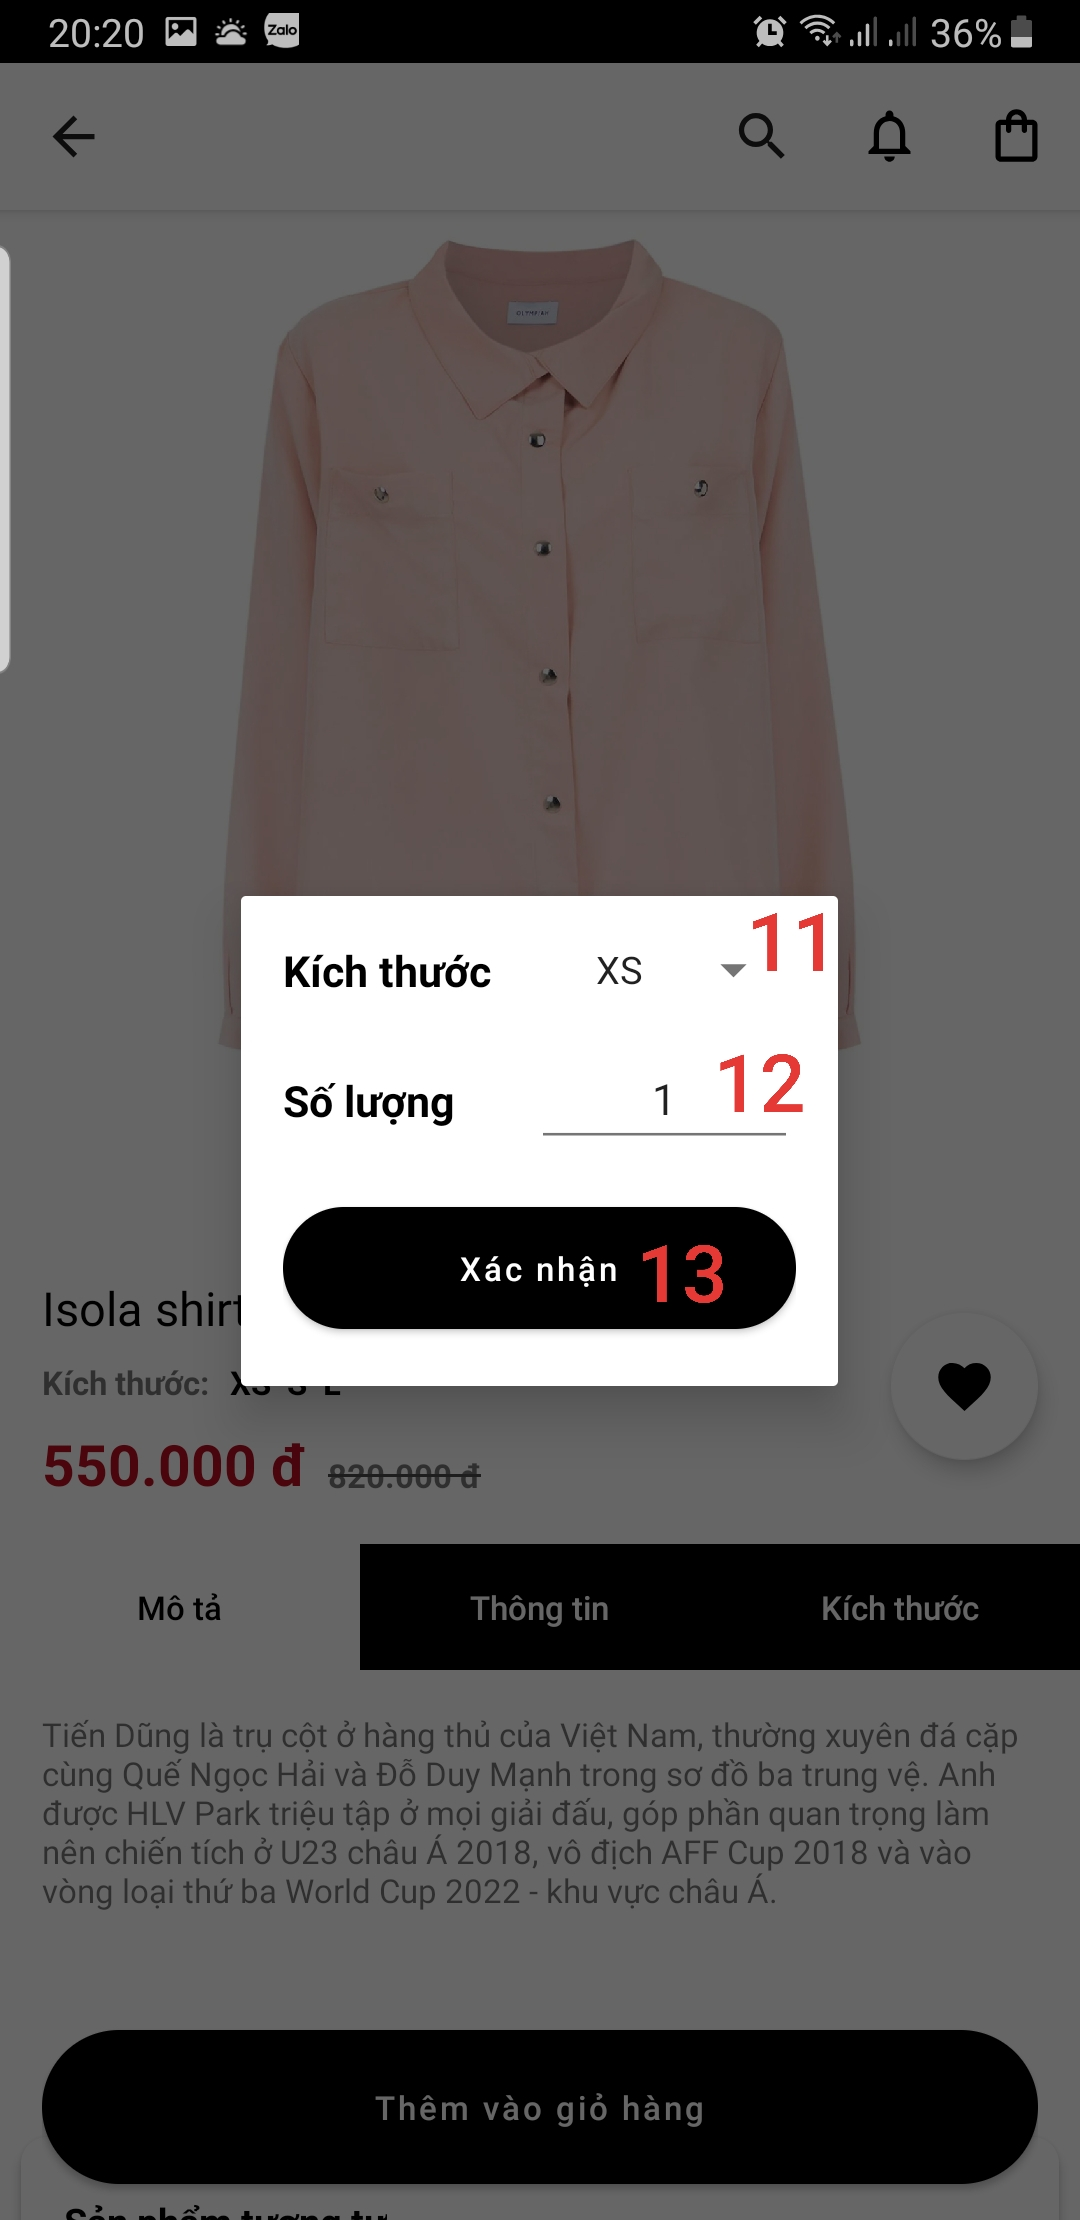
\includegraphics[height=0.7\textheight]{images/04.png}
            \caption{\centering\tiny{Hình 6: Màn hình chi tiết sản phẩm 3}}

        \end{figure}
        \column{0.7\linewidth}
        \indent \textbf{Các thành phần và chức năng kèm theo trên màn hình:}
        \begin{itemize}
            \item \textbf{11}: Spinner - cho phép người dùng chọn các size của sản phẩm.
            \item \textbf{12}: Text input - để người dùng nhập số lượng sản phẩm cần mua cho size tương ứng.
            \item \textbf{13}: Button - khi click vào sản phẩm sẽ được thêm vào giỏ hàng cùng size và số lượng đã chọn.
        \end{itemize}
    \end{columns}
\end{frame}

\begin{frame}
    \frametitle{Các màn hình và chức năng kèm theo (5)}
    \framesubtitle{Màn hình chi tiết sản phẩm - Mã nguồn minh họa}

    \begin{columns}
        \column{0.3\linewidth}
        \begin{figure}
            \centering
            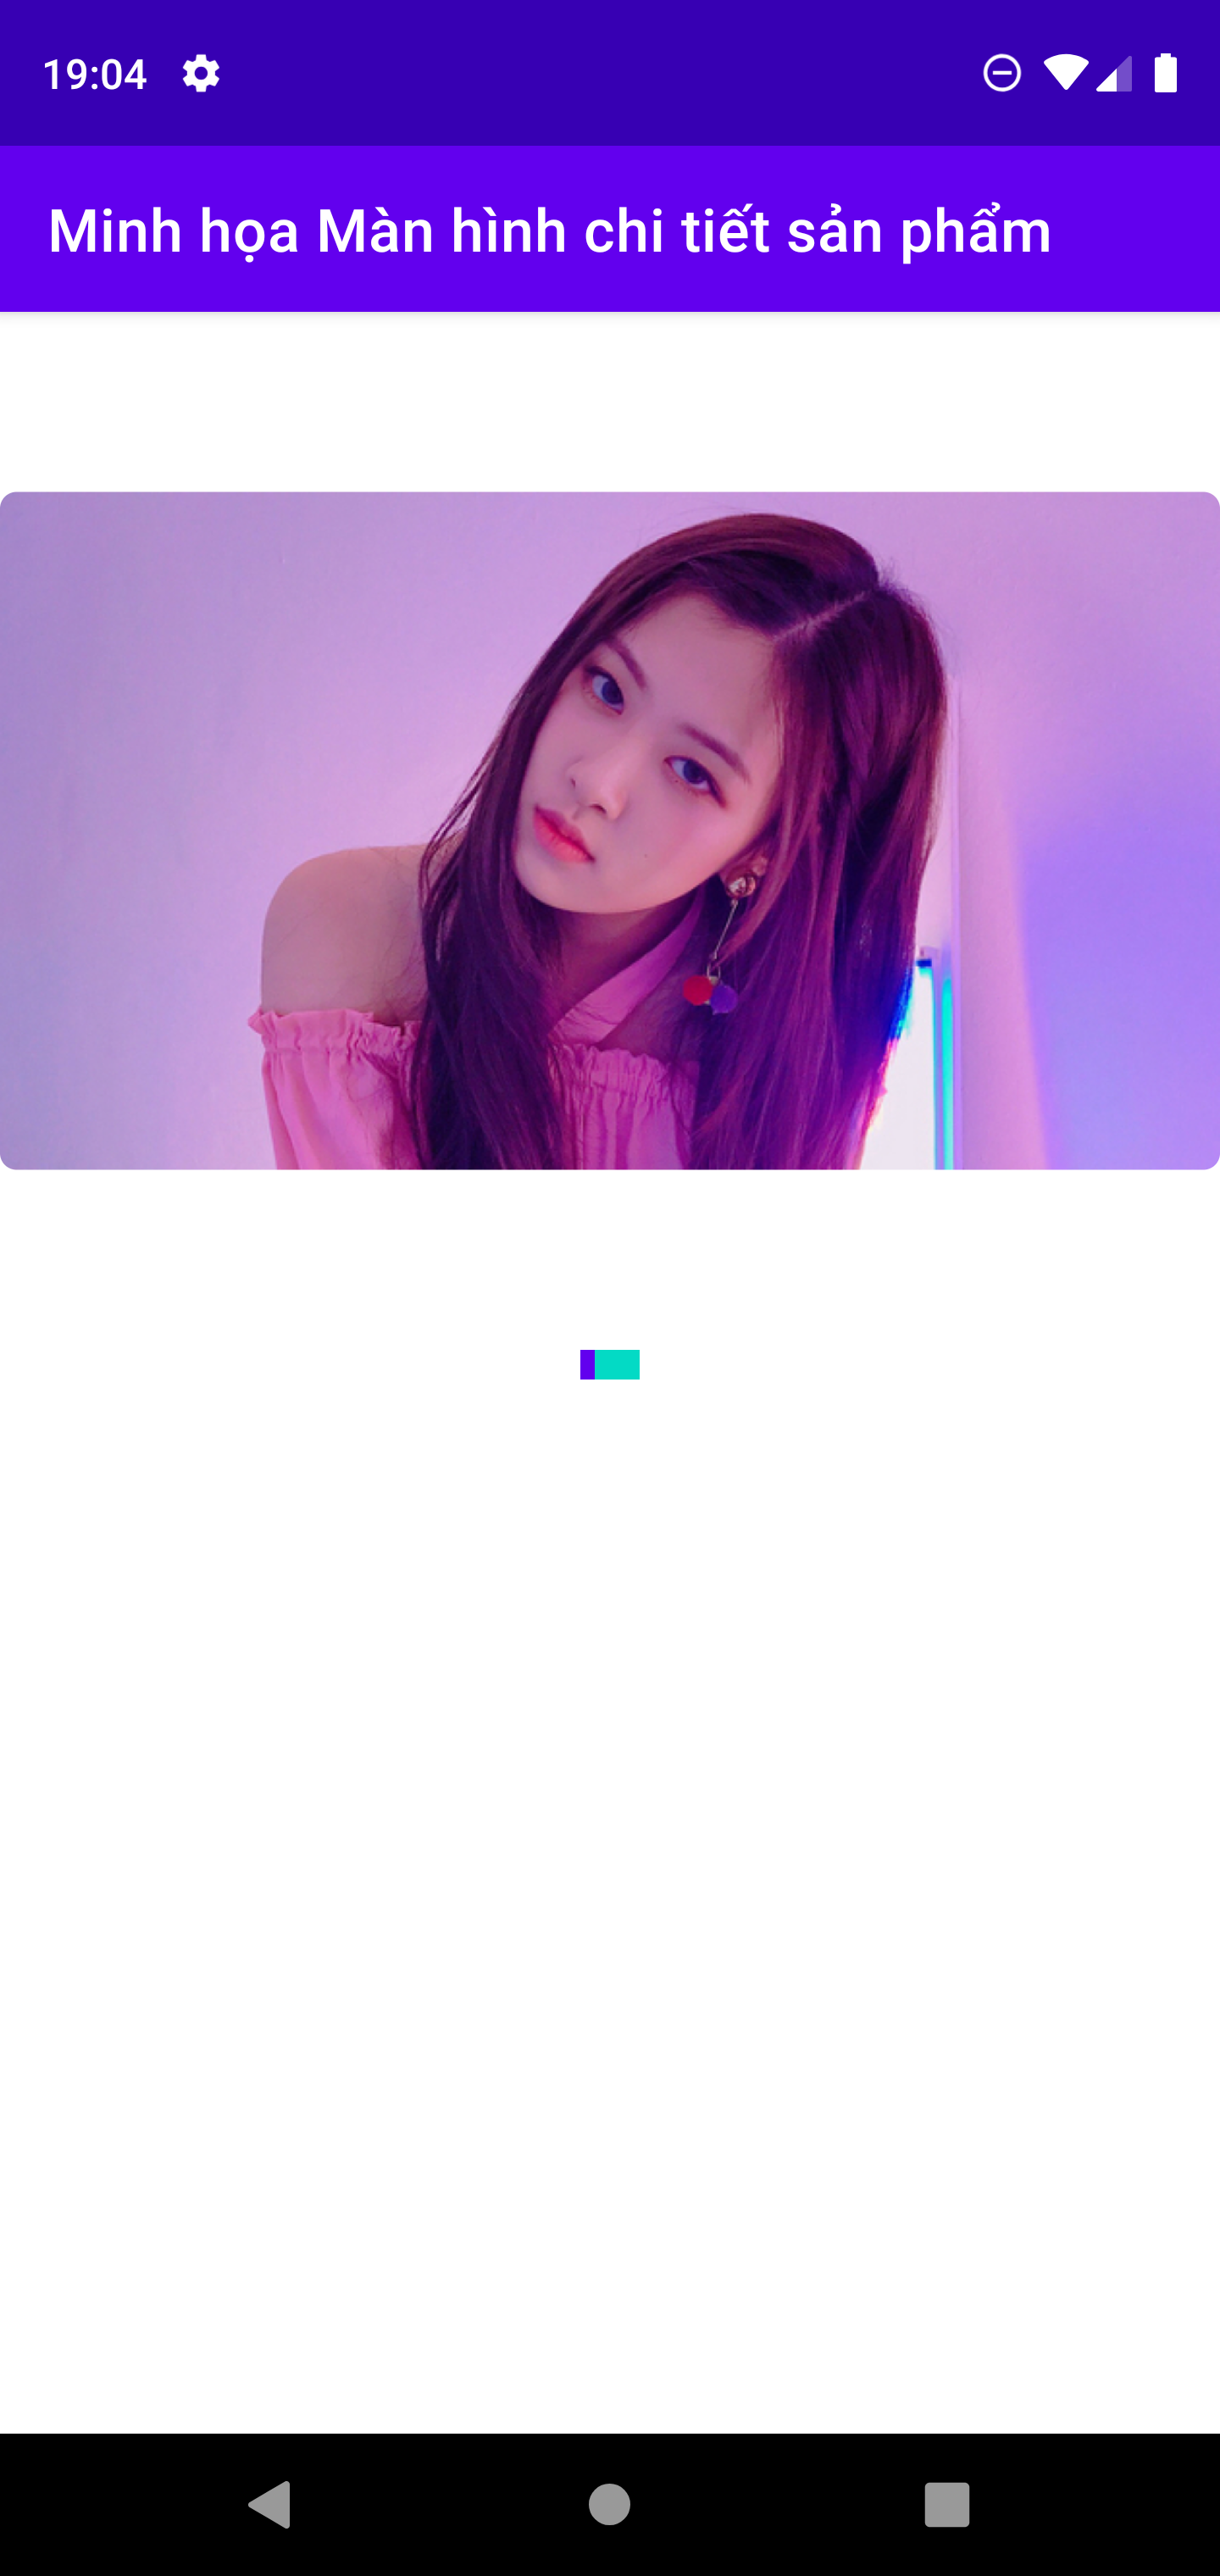
\includegraphics[height=0.7\textheight]{images/30.png}
            \caption{\centering\tiny{Hình 7: Minh họa màn hình chi tiết sản phẩm 1}}
        \end{figure}
        \column{0.7\linewidth}
        \indent Cấu trúc cây thư mục:
        \begin{figure}
            \centering
            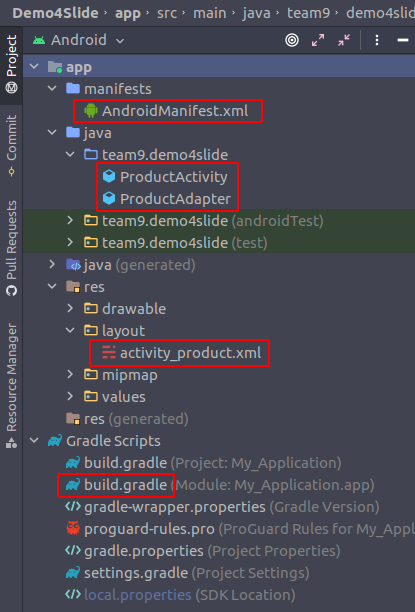
\includegraphics[height=0.68\textheight]{images/31.png}
        \end{figure}
    \end{columns}
\end{frame}

\begin{frame}
    \begin{columns}
        \column{0.3\linewidth}
        \begin{figure}
            \centering
            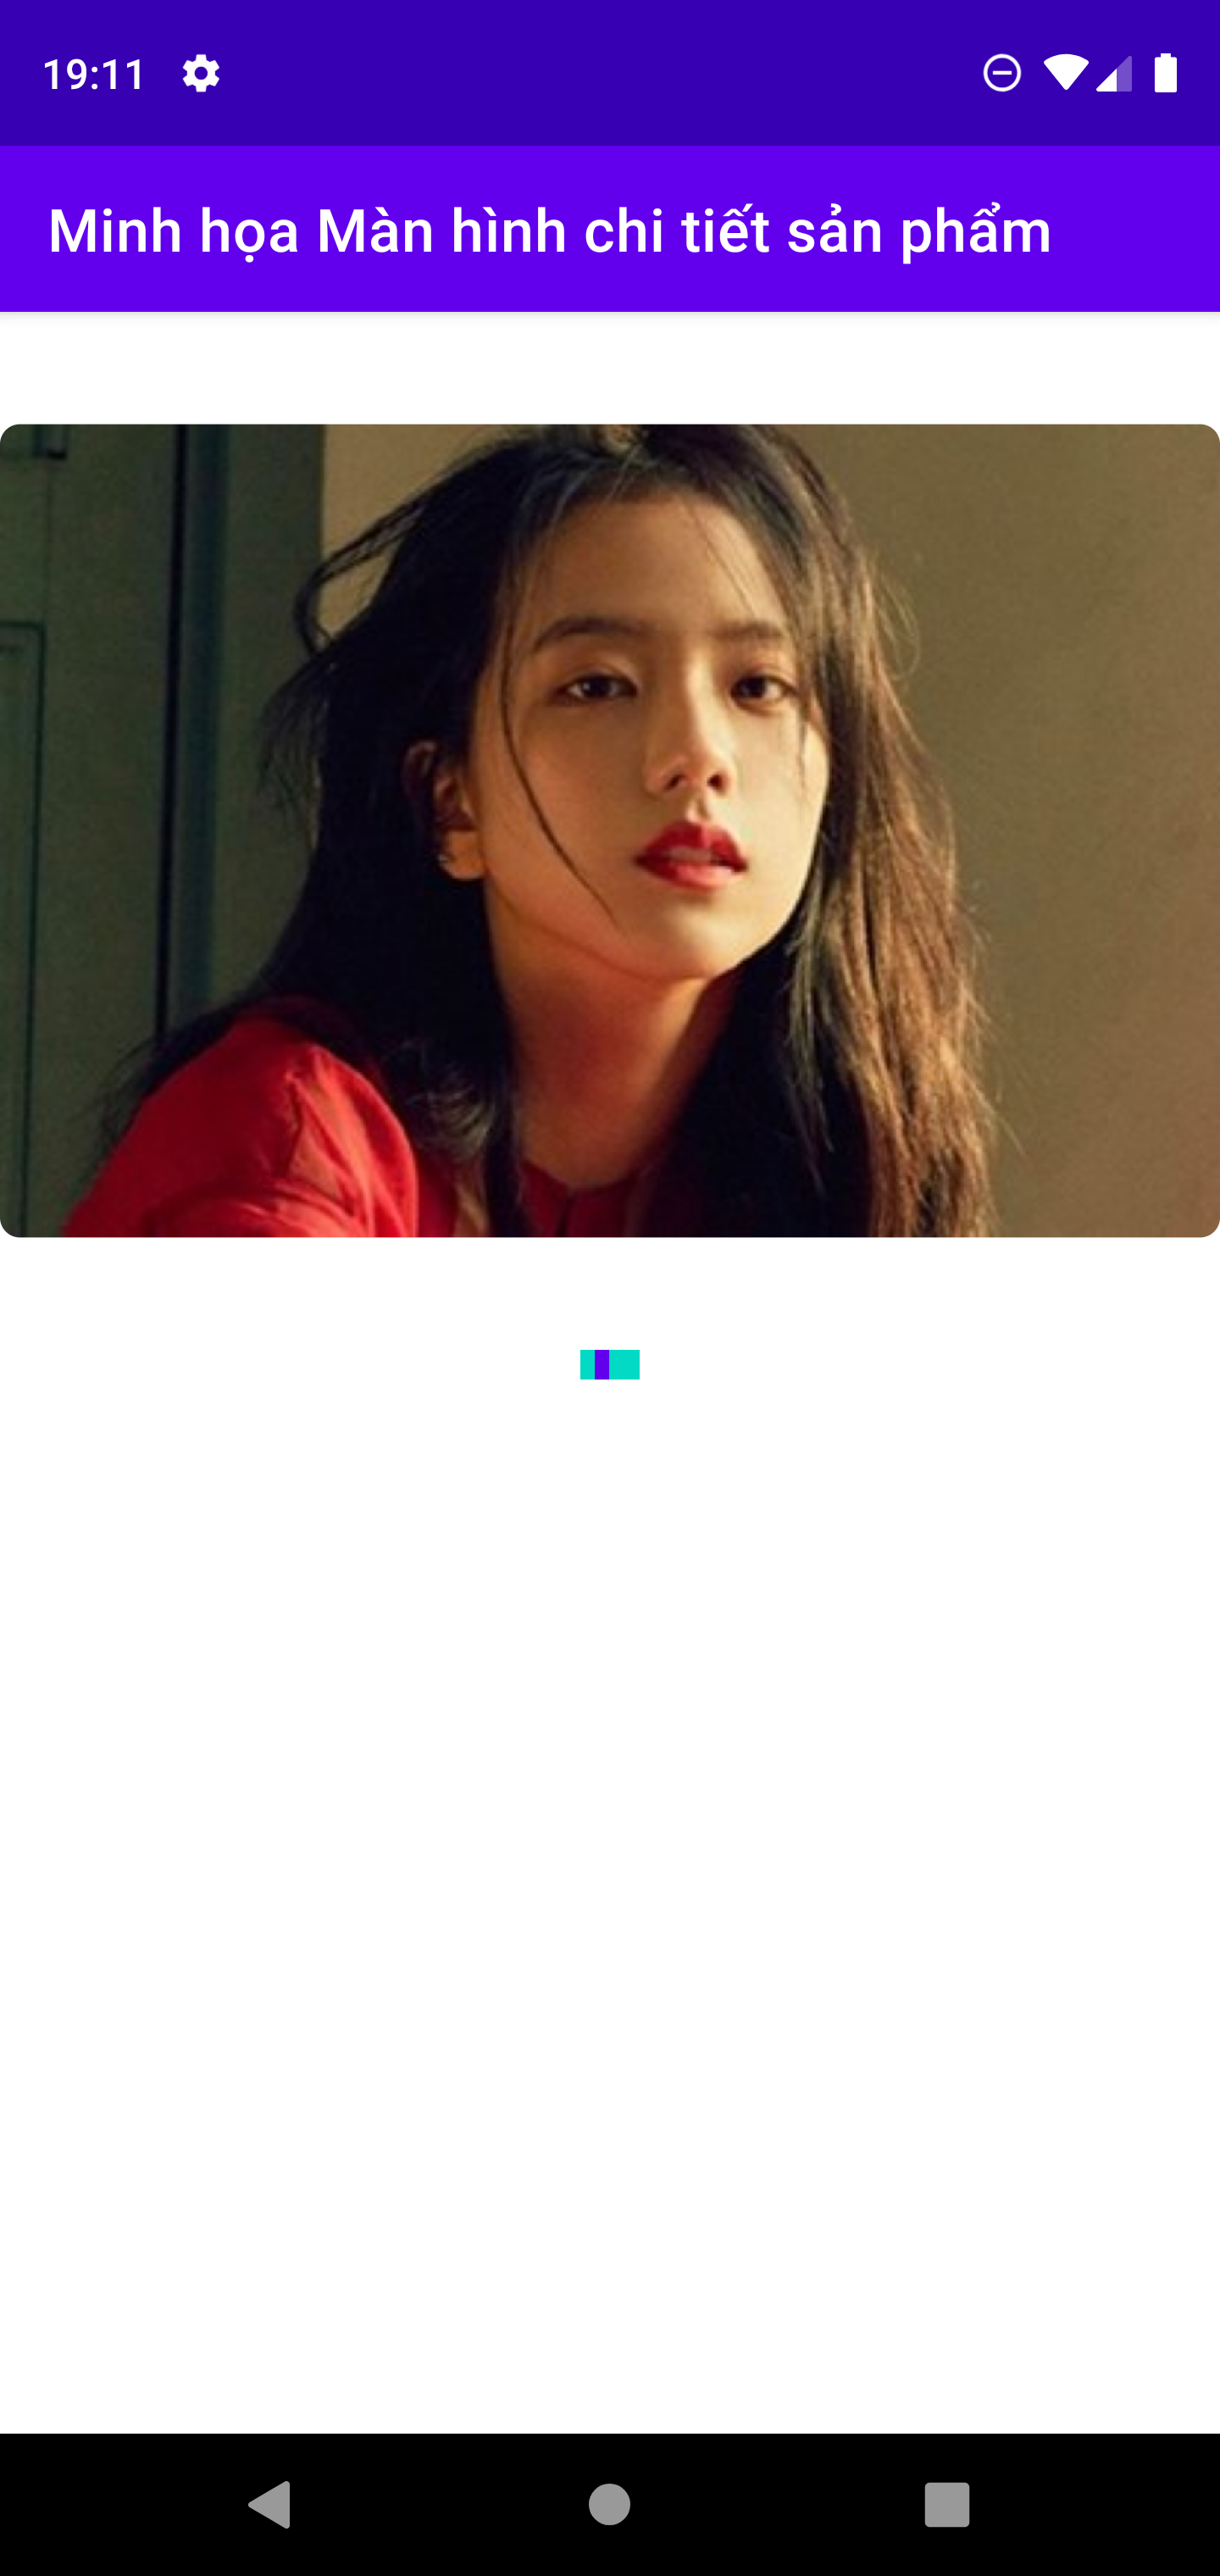
\includegraphics[height=0.7\textheight]{images/32.png}
            \caption{\centering\tiny{Hình 8: Minh họa màn hình chi tiết sản phẩm 2}}
        \end{figure}
        \column{0.7\linewidth}
        \indent \texttt{AndroidManifest.xml}
        \begin{figure}
            \centering
            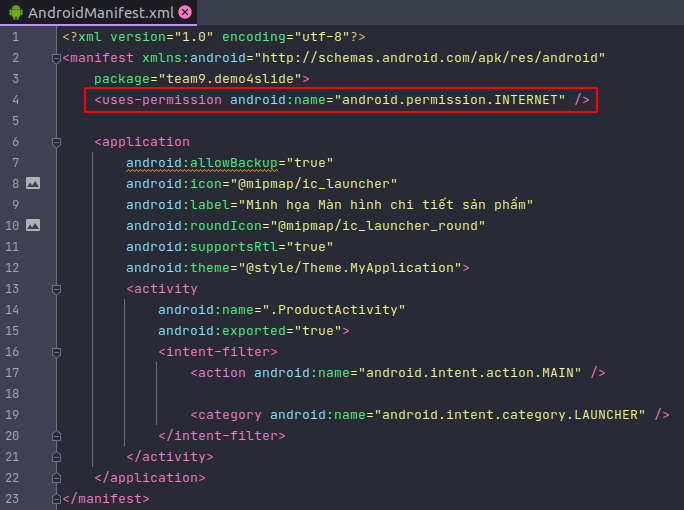
\includegraphics[width=\textwidth]{images/33.png}
        \end{figure}
    \end{columns}
\end{frame}

\begin{frame}
    \begin{columns}
        \column{0.3\linewidth}
        \begin{figure}
            \centering
            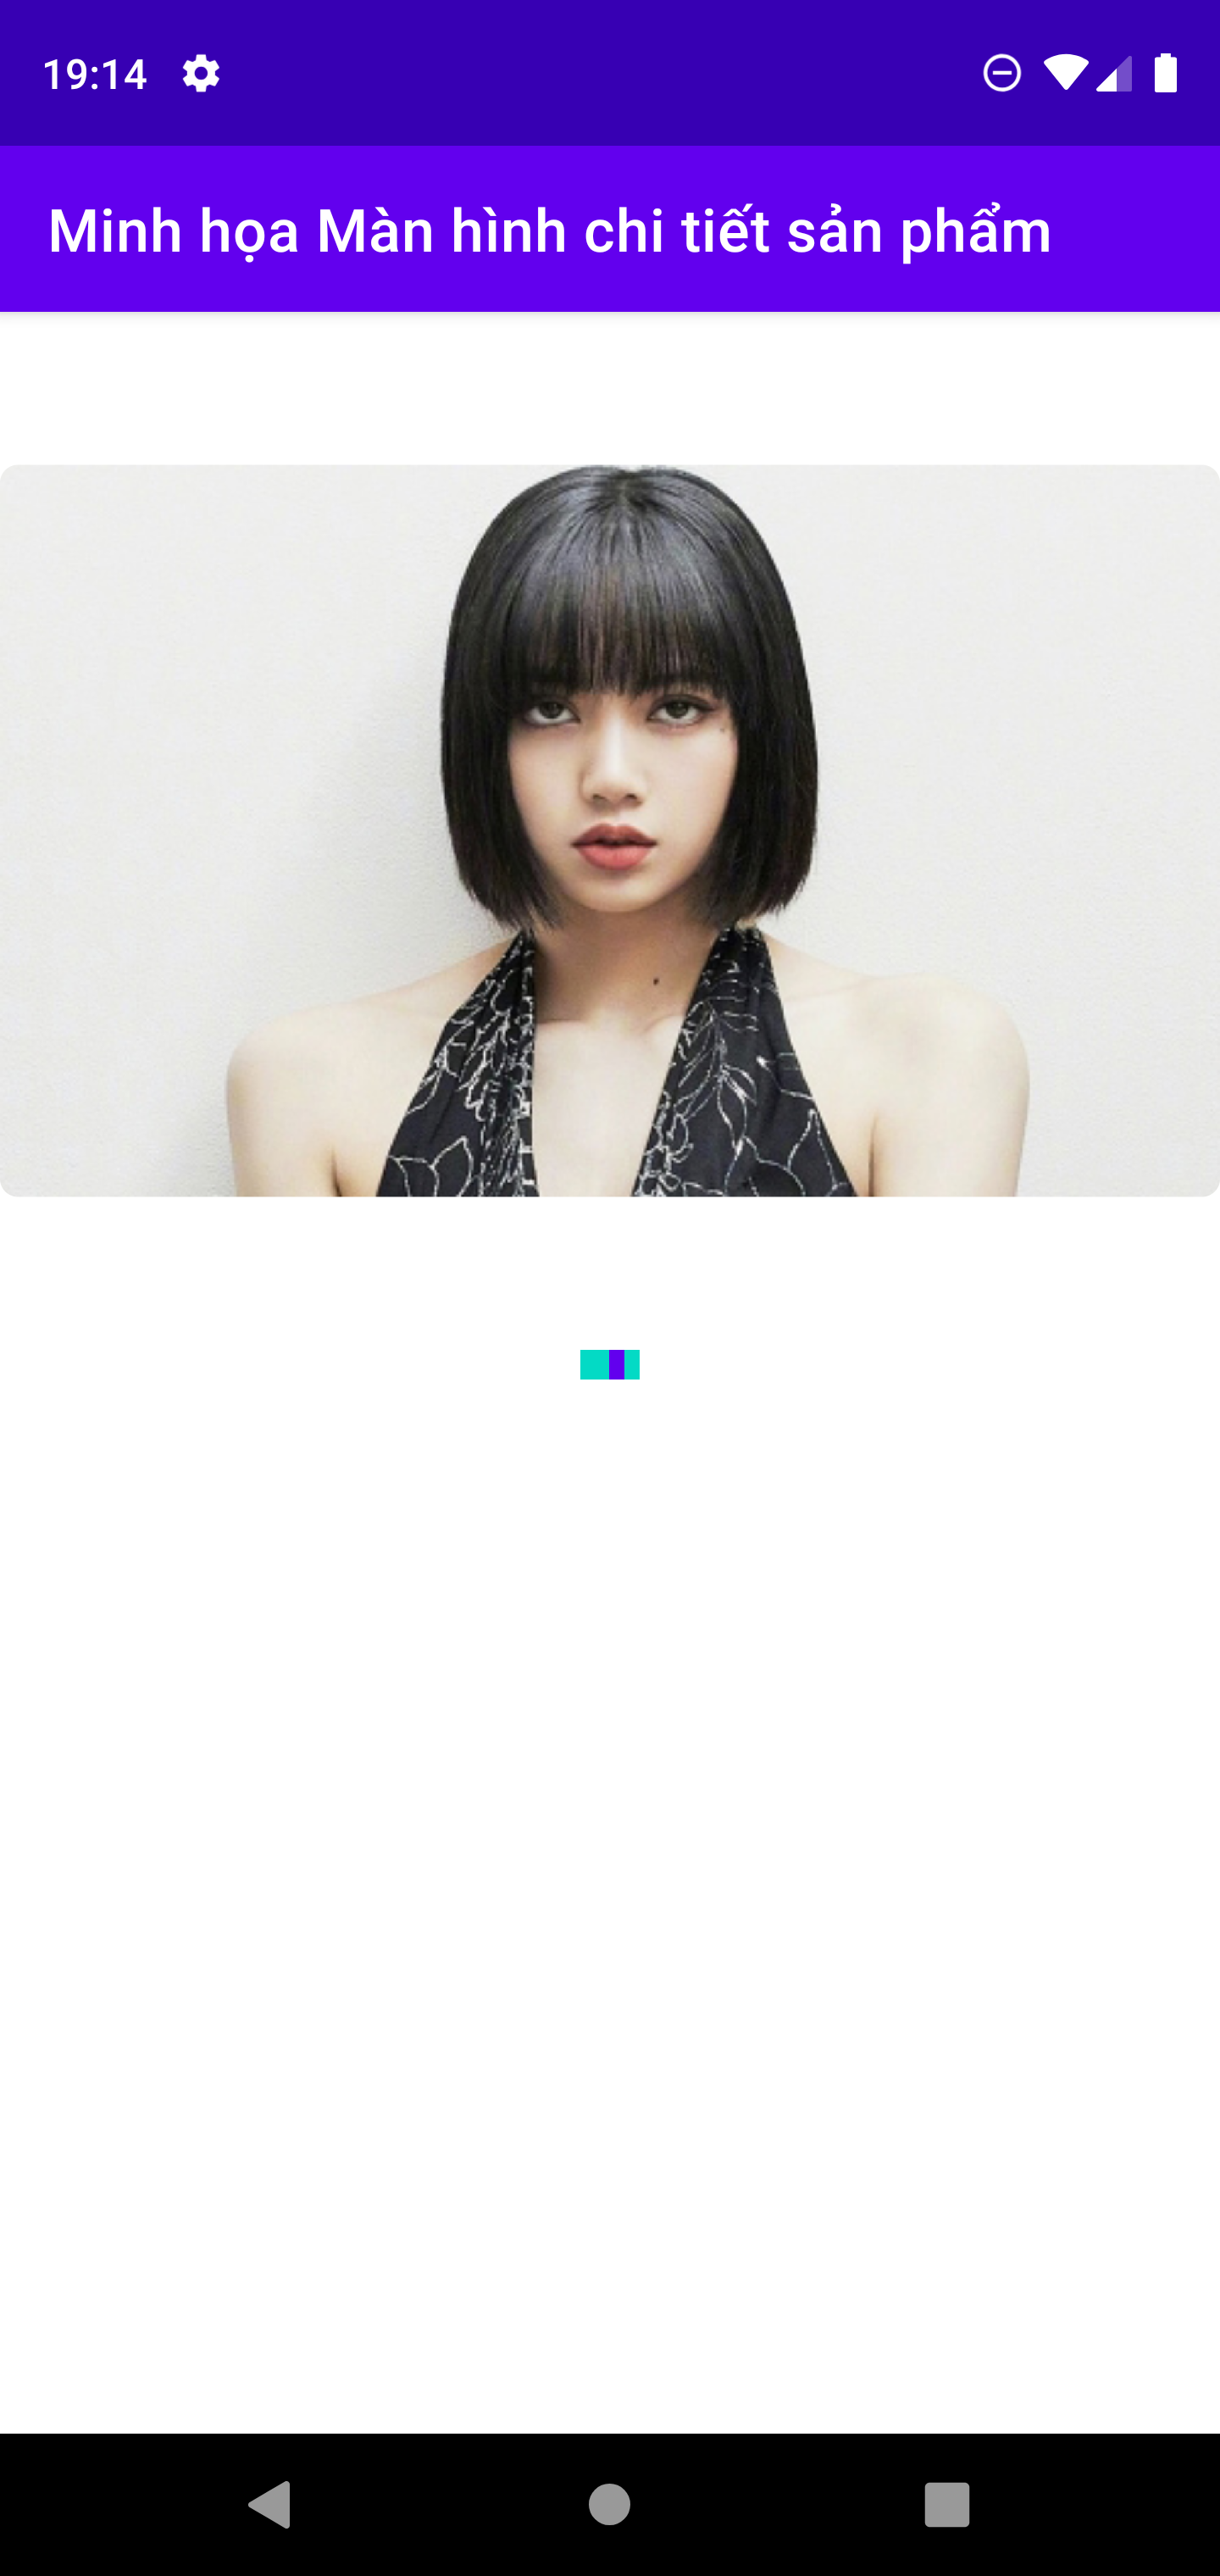
\includegraphics[height=0.7\textheight]{images/34.png}
            \caption{\centering\tiny{Hình 9: Minh họa màn hình chi tiết sản phẩm 3}}
        \end{figure}
        \column{0.7\linewidth}
        \indent \texttt{build.gradle}
        \begin{figure}
            \centering
            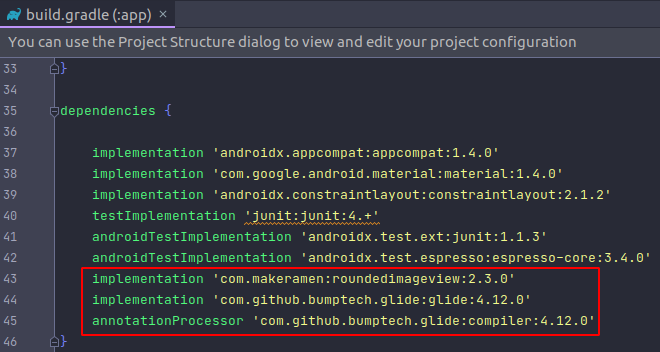
\includegraphics[width=\textwidth]{images/35.png}
        \end{figure}
    \end{columns}
\end{frame}

\begin{frame}
    \begin{columns}
        \column{0.3\linewidth}
        \begin{figure}
            \centering
            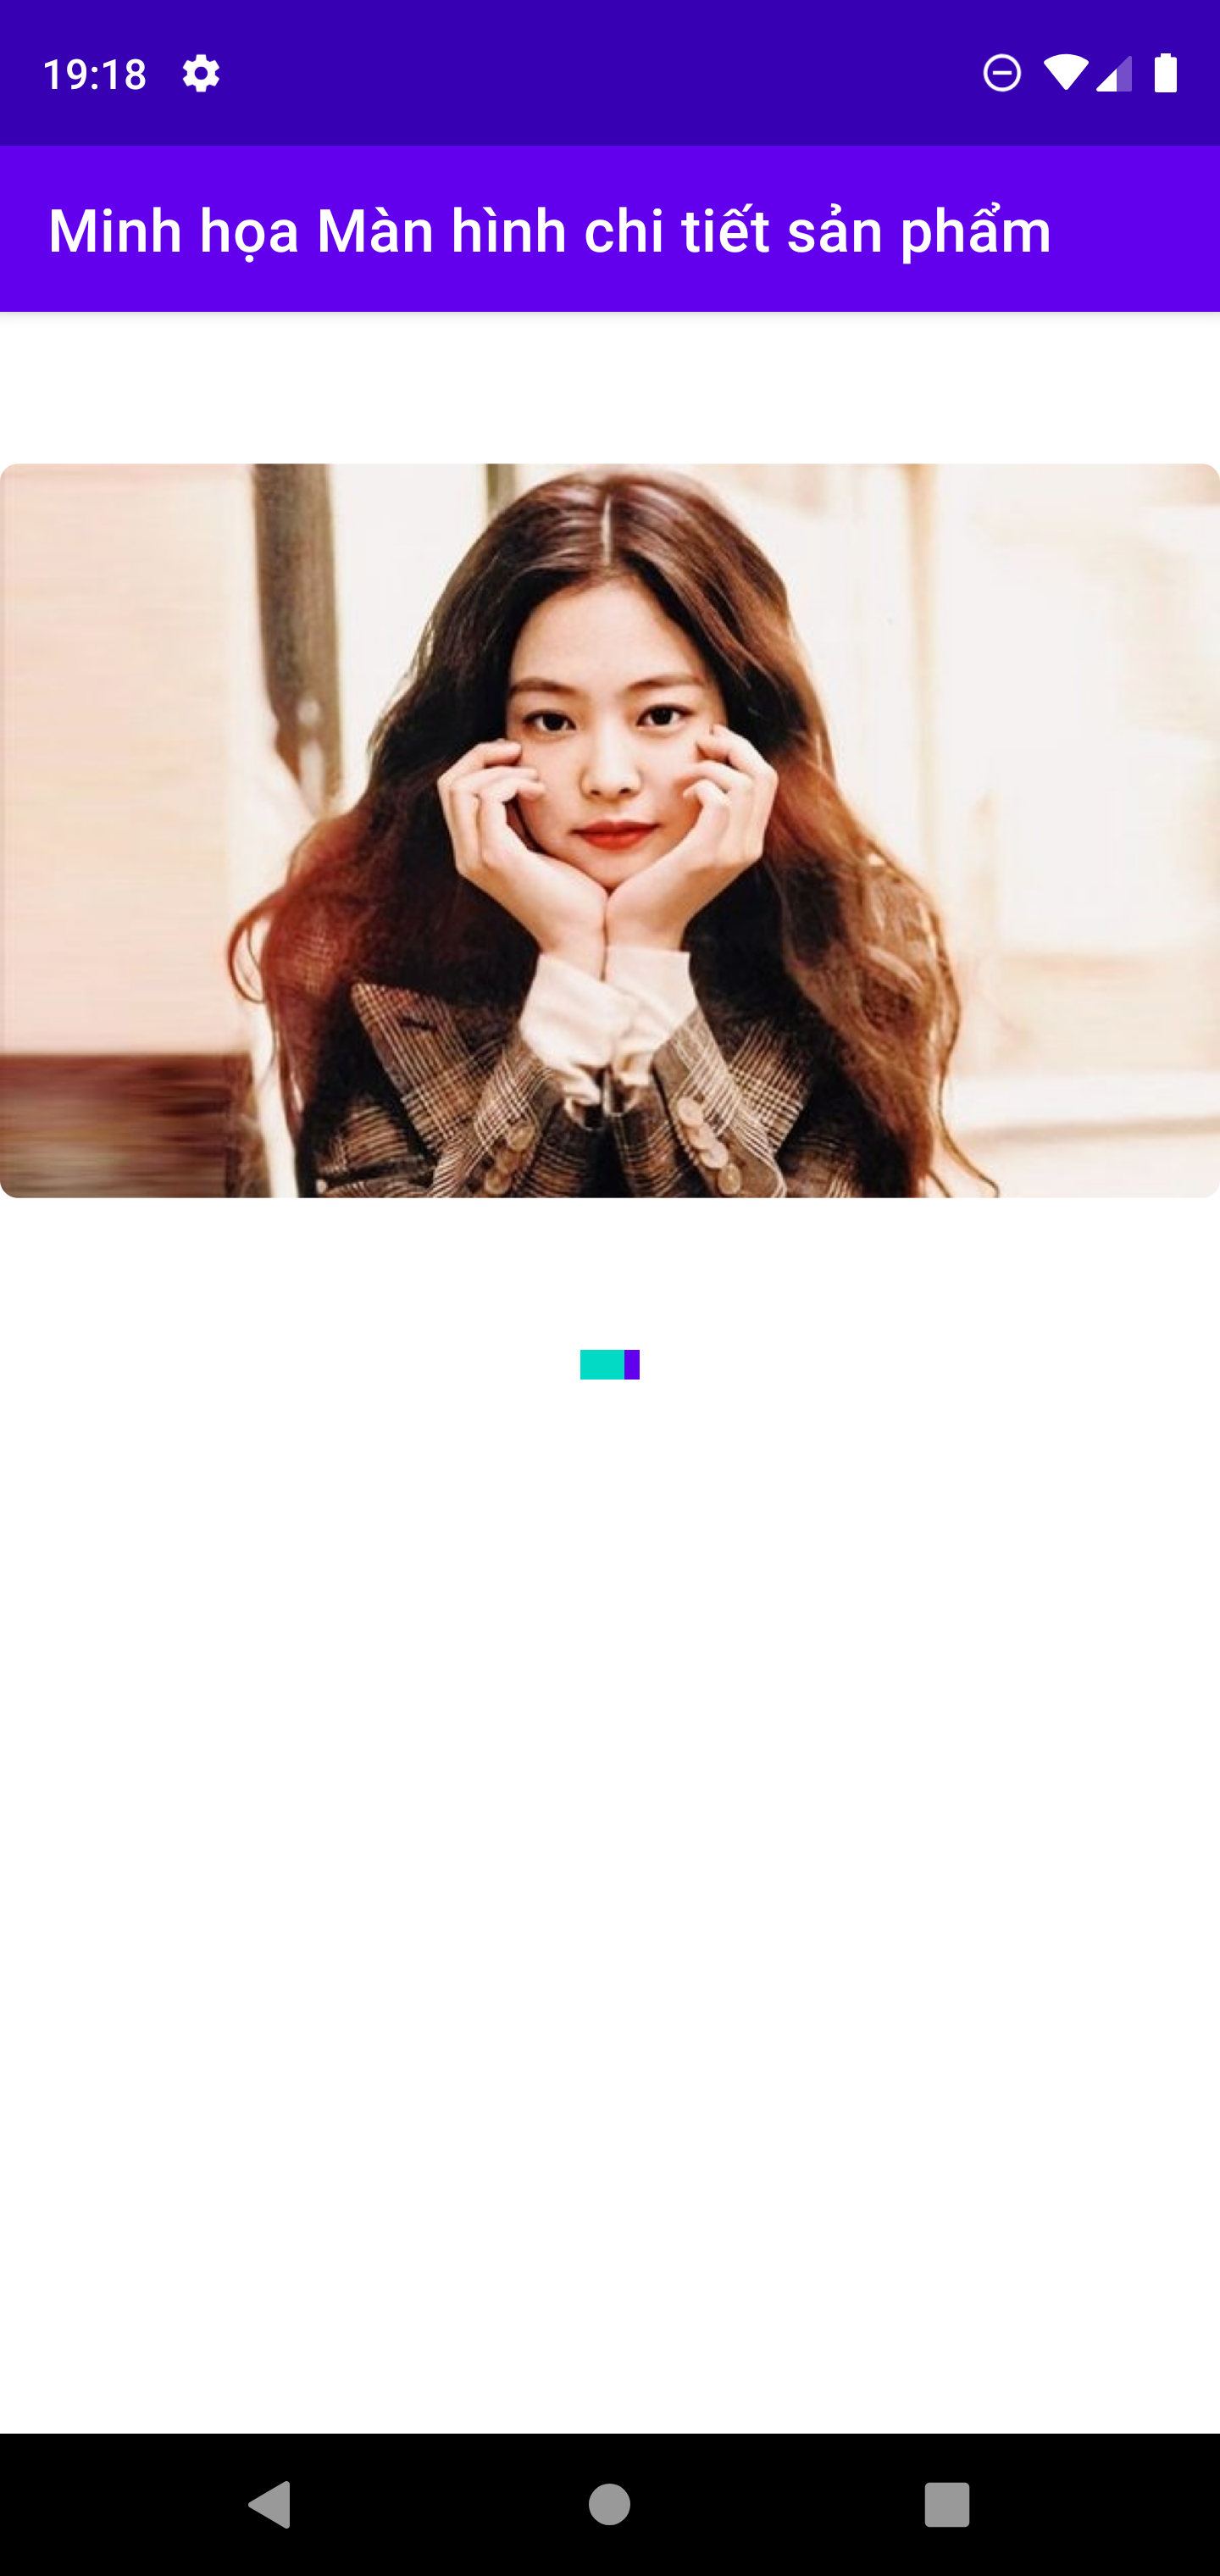
\includegraphics[height=0.7\textheight]{images/37.png}
            \caption{\centering\tiny{Hình 10: Minh họa màn hình chi tiết sản phẩm 4}}
        \end{figure}
        \column{0.7\linewidth}
        \indent \texttt{activity\_product.xml}
        \begin{figure}
            \centering
            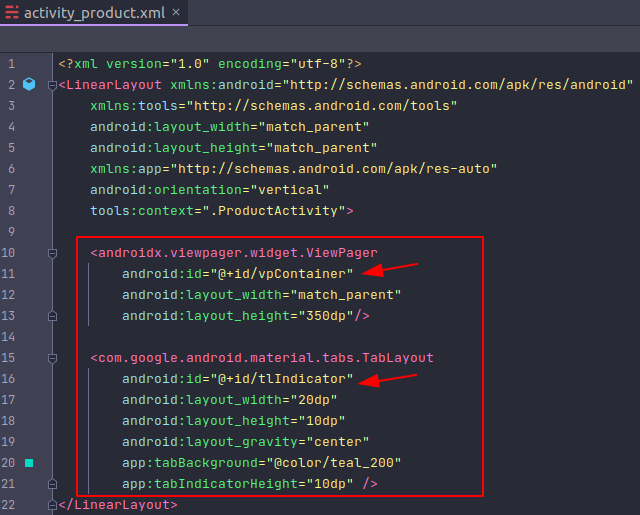
\includegraphics[width=\textwidth]{images/36.png}
        \end{figure}
    \end{columns}
\end{frame}

\begin{frame}
    \begin{columns}
        \column{0.3\linewidth}
        \begin{figure}
            \centering
            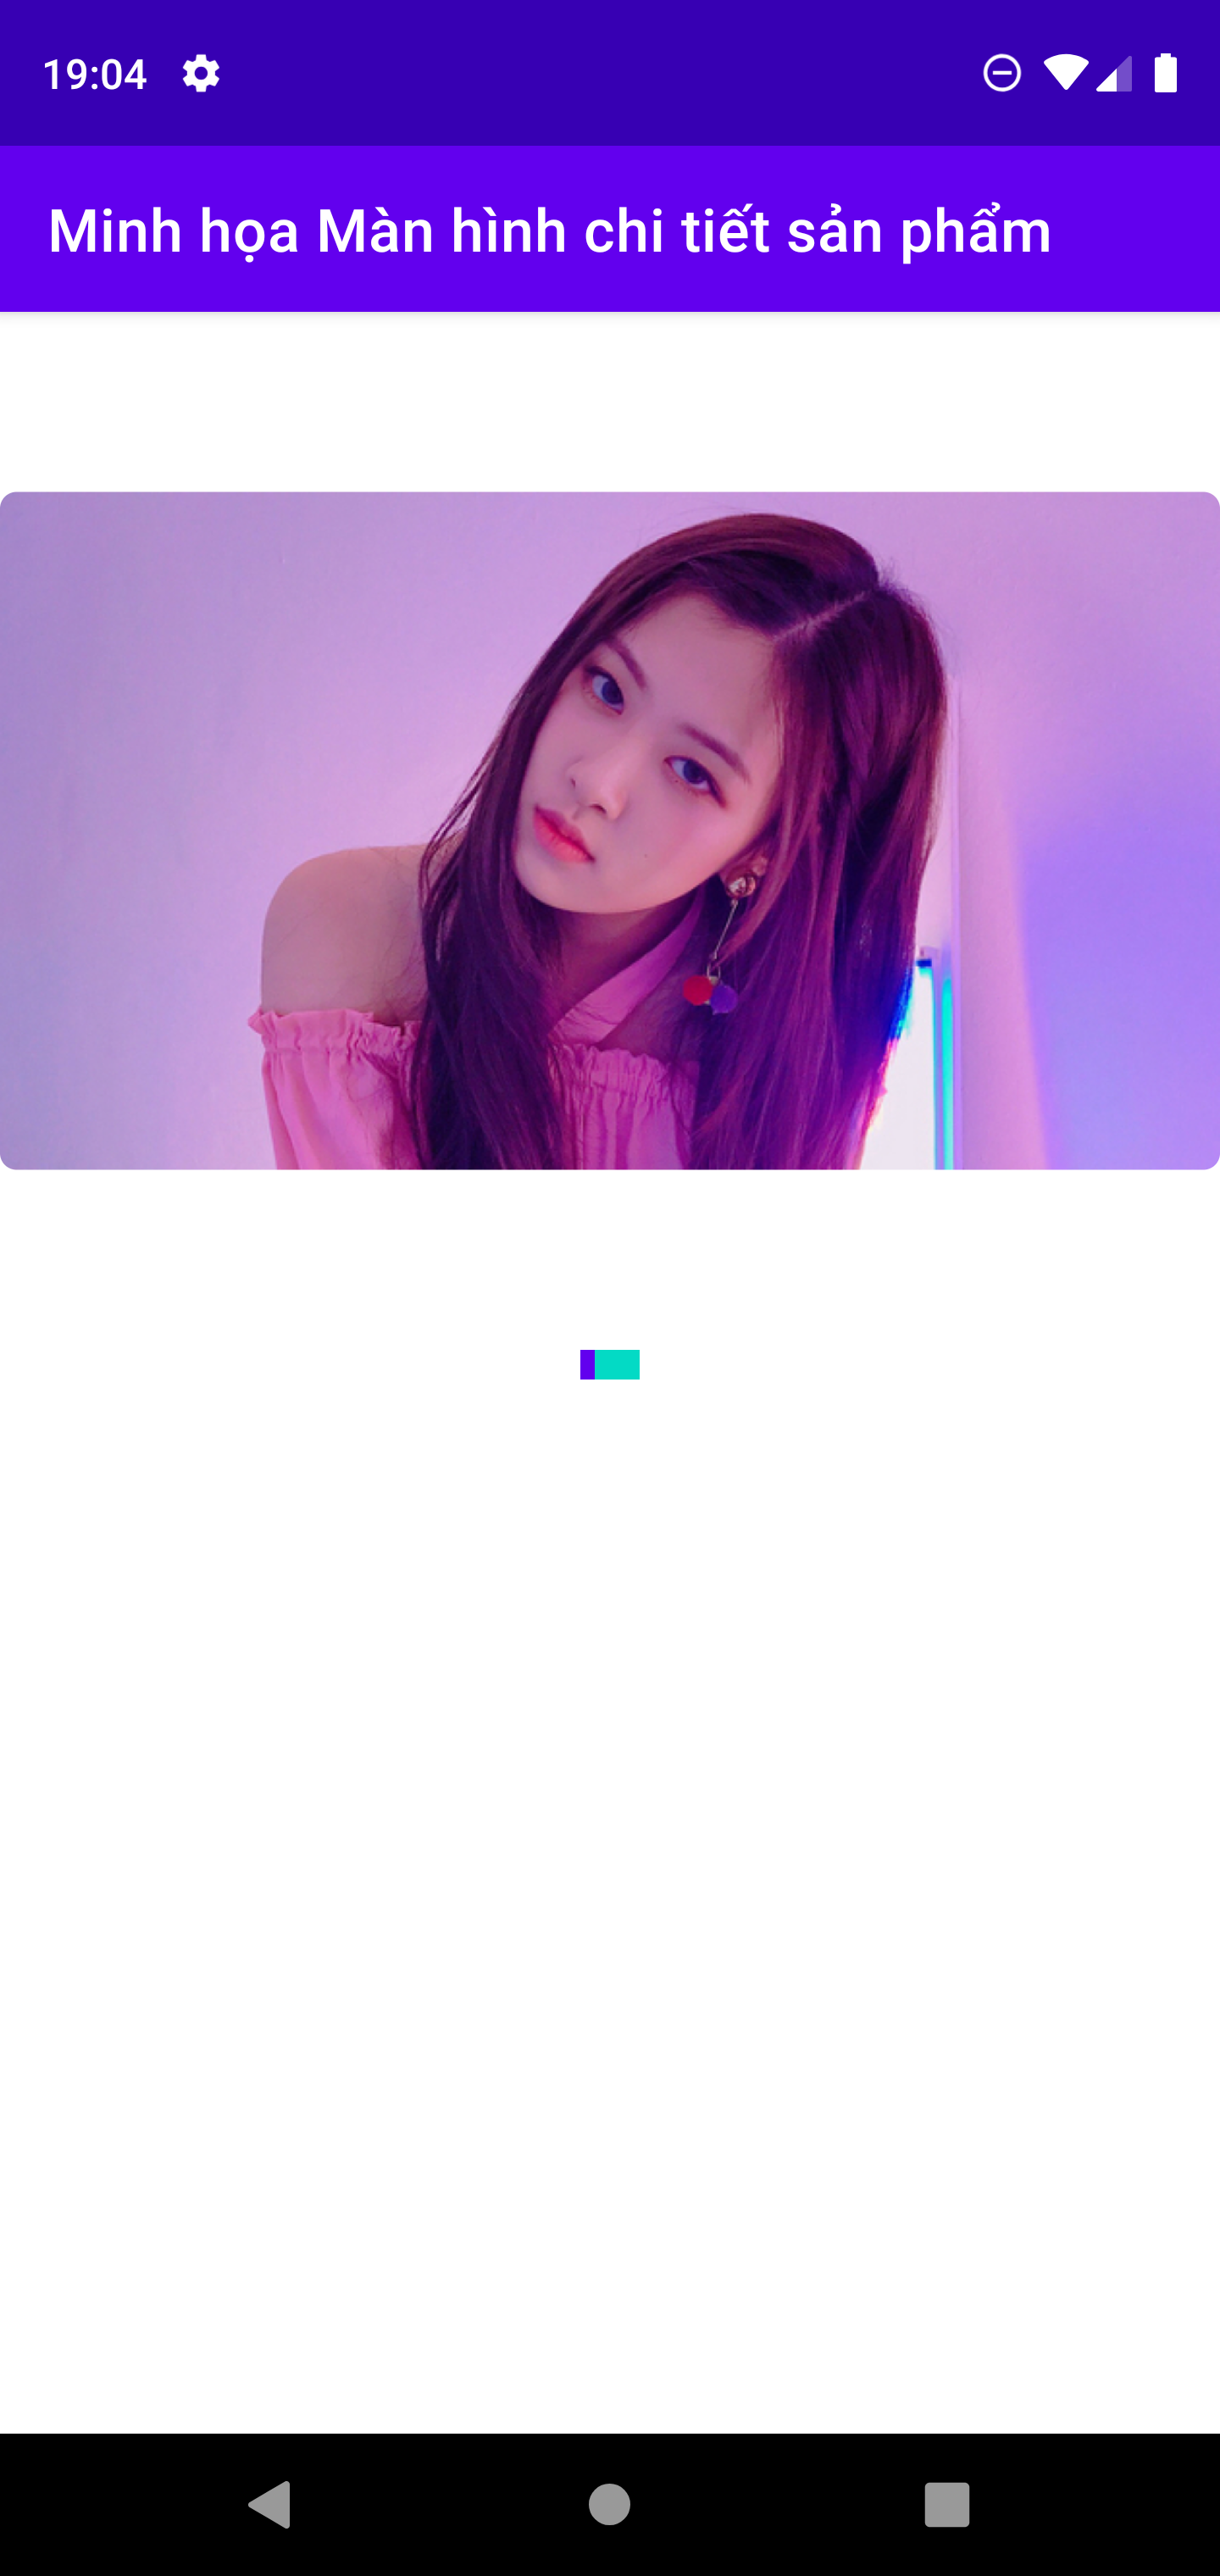
\includegraphics[height=0.7\textheight]{images/30.png}
            \caption{\centering\tiny{Hình 7: Minh họa màn hình chi tiết sản phẩm 1}}
        \end{figure}
        \column{0.7\linewidth}
        \indent \texttt{ProductAdapter.java}
        \begin{figure}
            \centering
            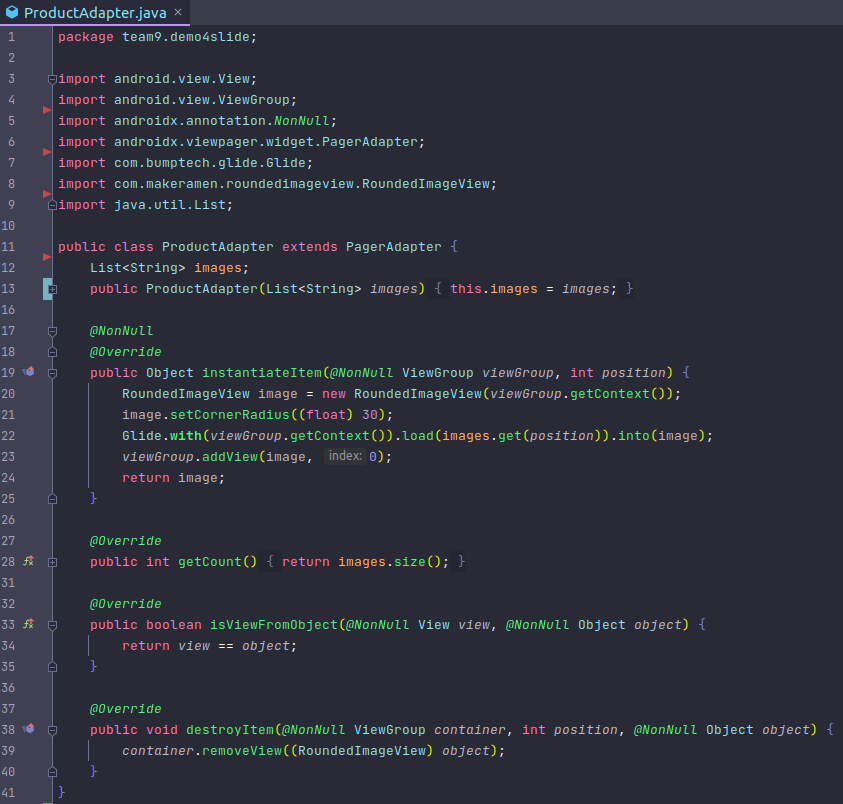
\includegraphics[width=\textwidth]{images/38.png}
        \end{figure}
    \end{columns}
\end{frame}

\begin{frame}
    \begin{columns}
        \column{0.3\linewidth}
        \begin{figure}
            \centering
            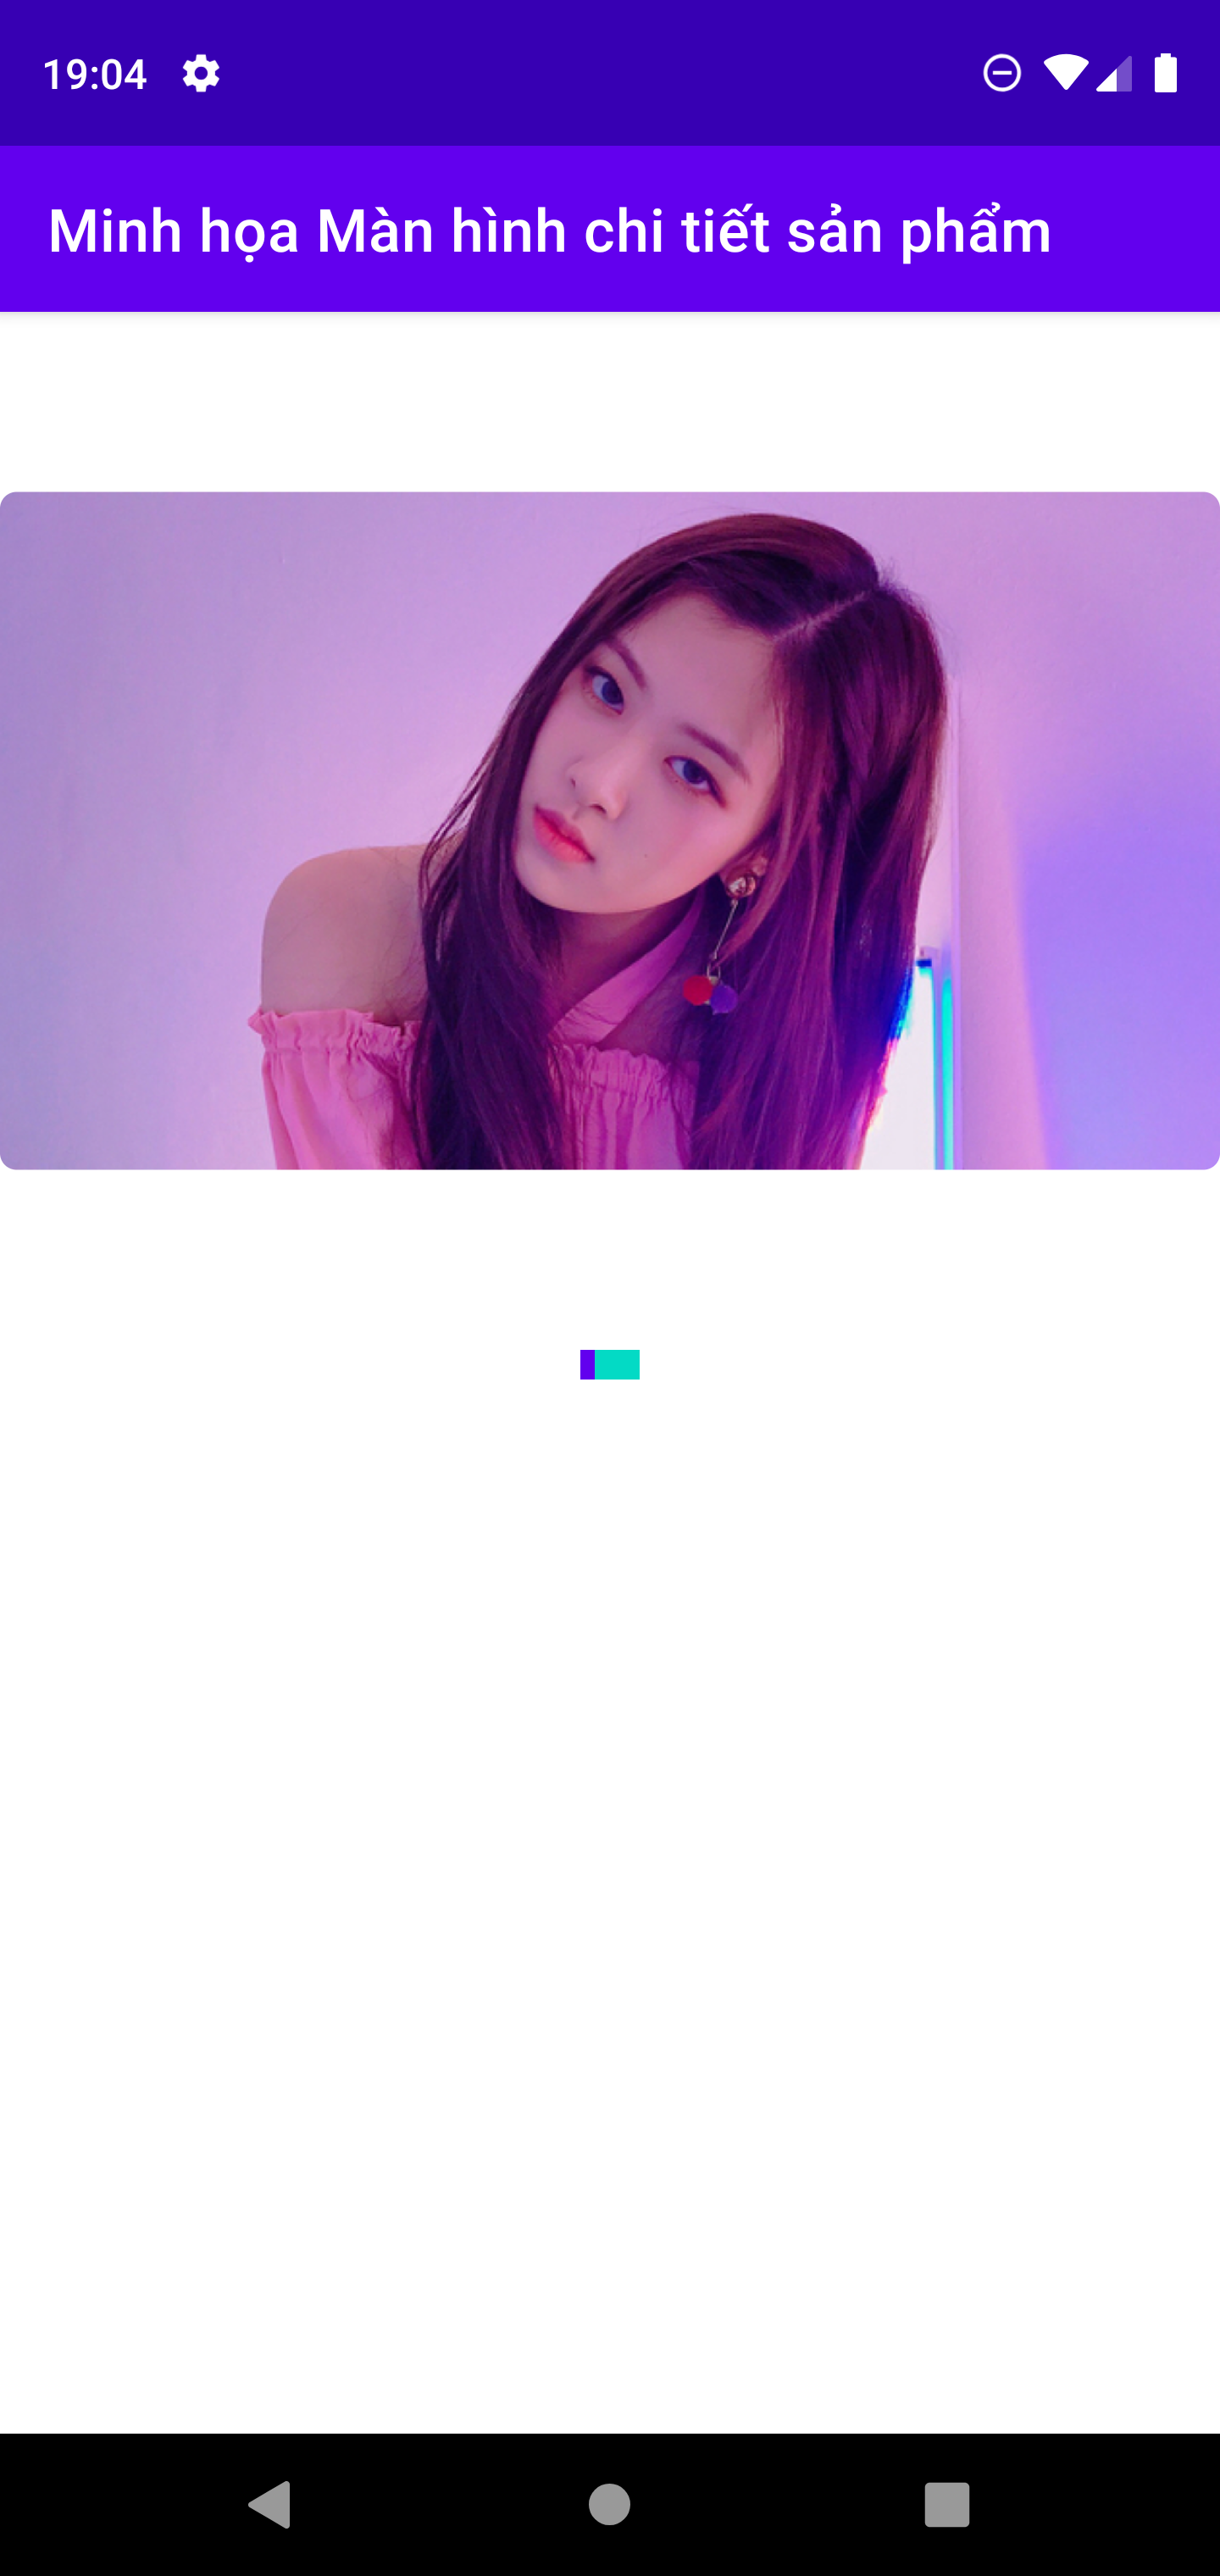
\includegraphics[height=0.7\textheight]{images/30.png}
            \caption{\centering\tiny{Hình 7: Minh họa màn hình chi tiết sản phẩm 1}}
        \end{figure}
        \column{0.7\linewidth}
        \indent \texttt{ProductActivity.java}
        \begin{figure}
            \centering
            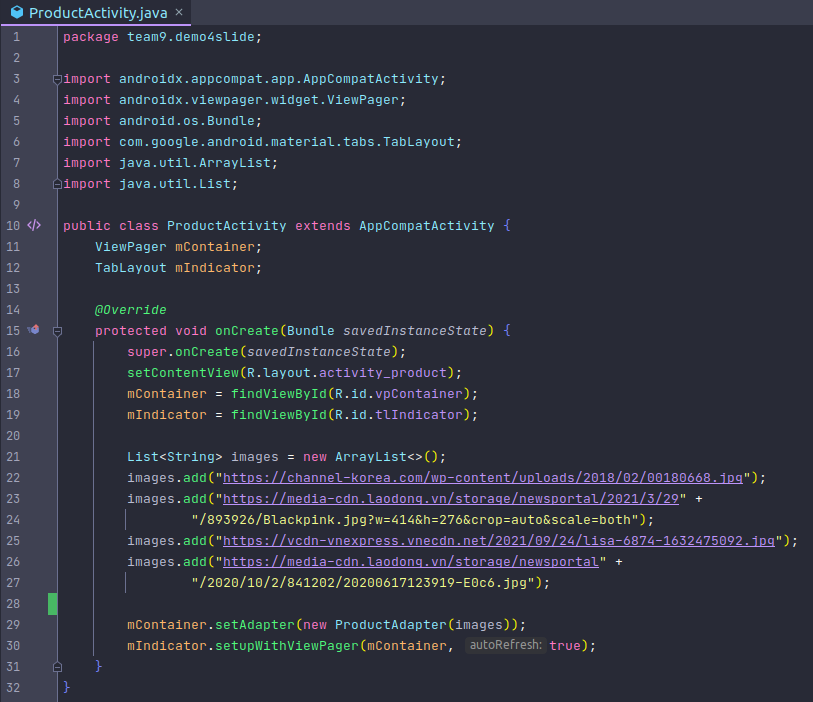
\includegraphics[width=\textwidth]{images/39.png}
        \end{figure}
    \end{columns}
\end{frame}

% =========================================================================== Slide 13
\begin{frame}
    \frametitle{Các màn hình và chức năng kèm theo (6)}
    \framesubtitle{Màn hình chính}

    \begin{columns}
        \column{0.3\linewidth}
        \begin{figure}
            \centering
            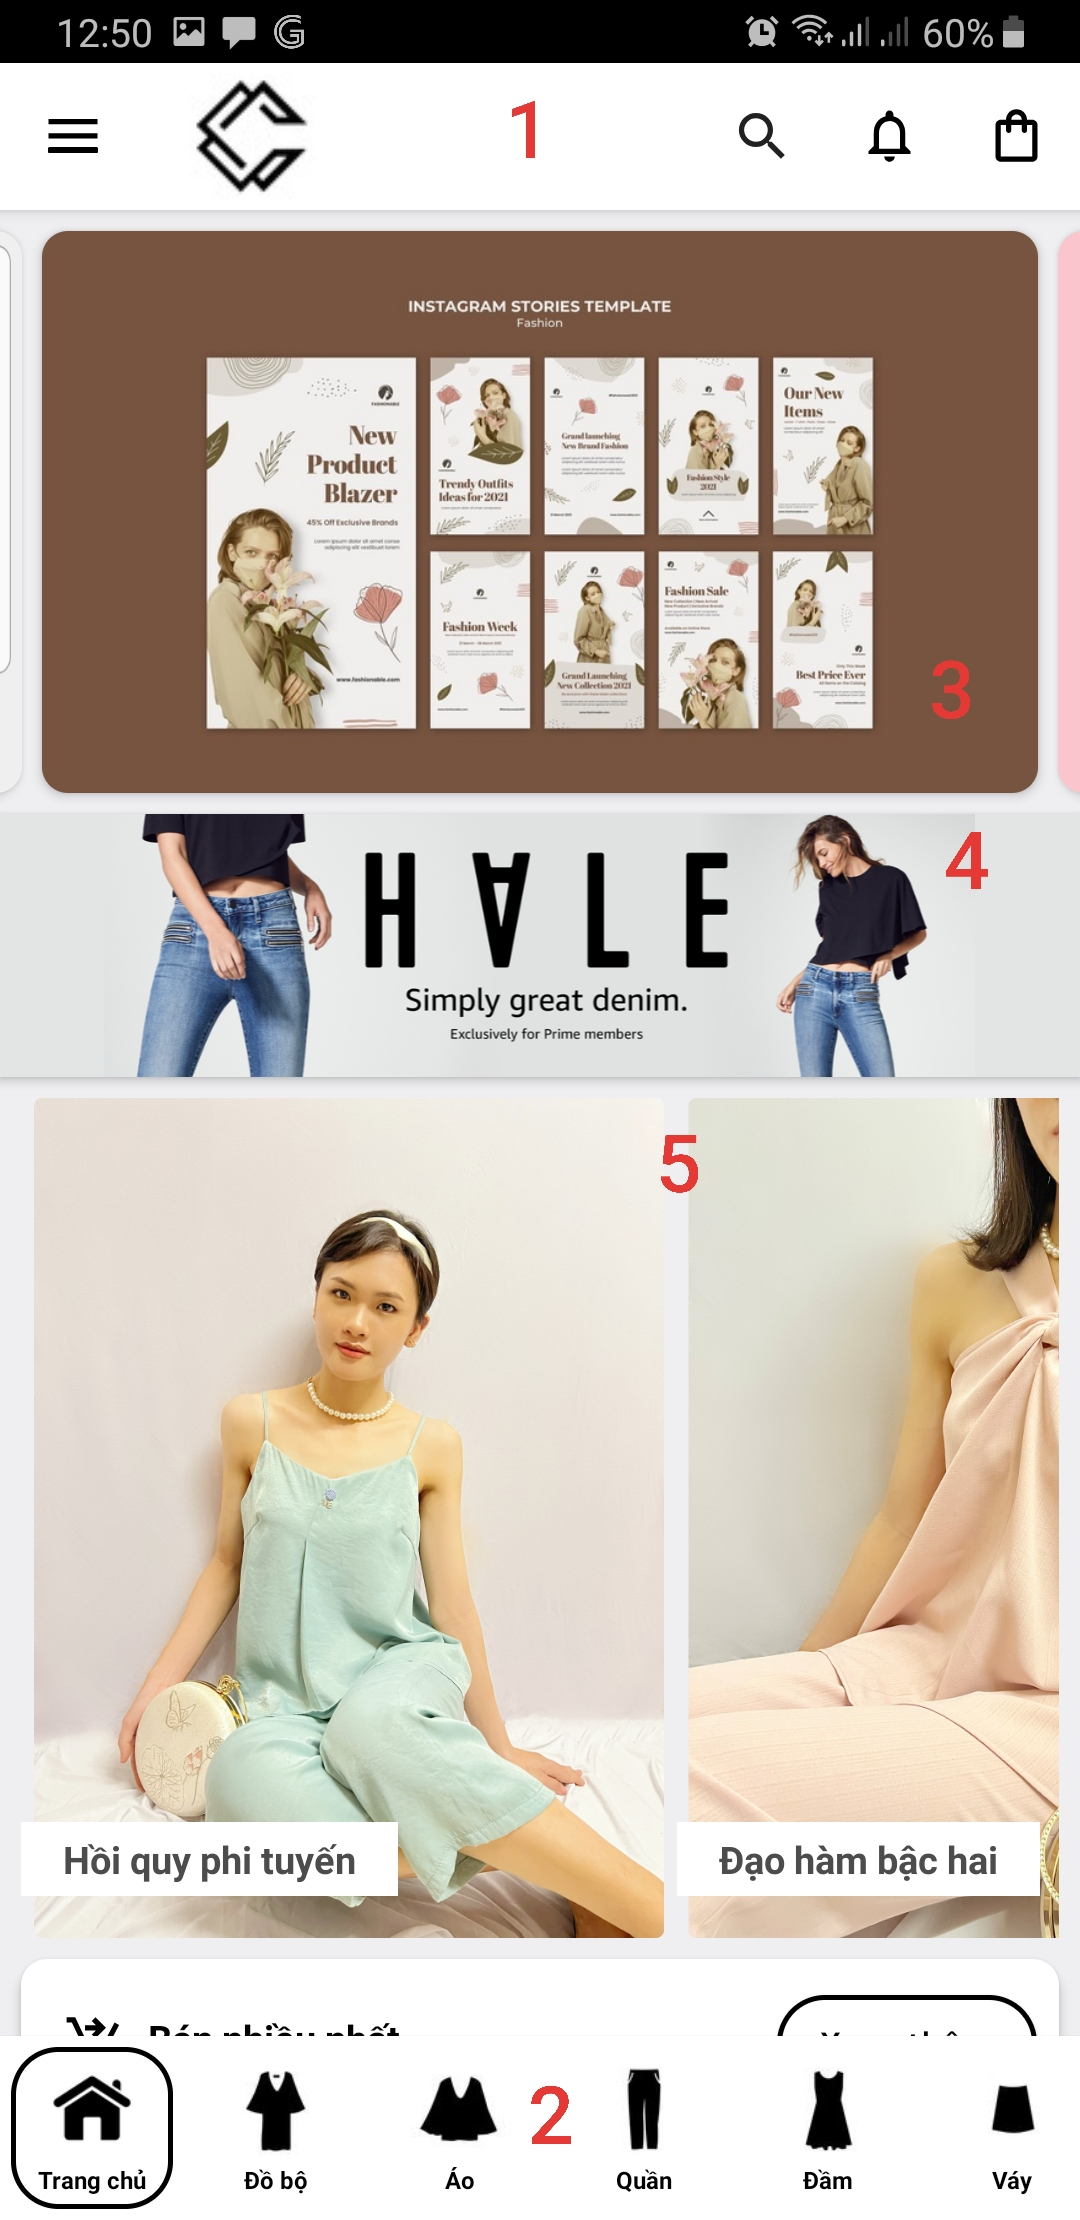
\includegraphics[height=0.7\textheight]{images/06.png}
            \caption{\centering\tiny{Hình 11: Màn hình chính của ứng dụng 1}}

        \end{figure}
        \column{0.7\linewidth}
        \indent \textbf{Các thành phần và chức năng kèm theo trên màn hình:}
        \begin{itemize}
            \item \textbf{1}: Action bar - chứa các thành phần từ trái qua phải như sau:
                  \begin{itemize}
                      \item Hamburger toggle - nhấn vào để mở navigation view.
                      \item Actionbar logo - hiển thị logo của ứng dụng.
                      \item Menu item Search - chức năng tìm kiếm.
                      \item Menu item Notification - chức năng thông báo (chưa hỗ trợ do ứng dụng chưa có web service + server xử lí).
                      \item Menu item Cart - bấm vào để đi đến fragment giỏ hàng.
                  \end{itemize}
        \end{itemize}
    \end{columns}
\end{frame}

% =========================================================================== Slide 12
\begin{frame}
    \begin{columns}
        \column{0.3\linewidth}
        \begin{figure}
            \centering
            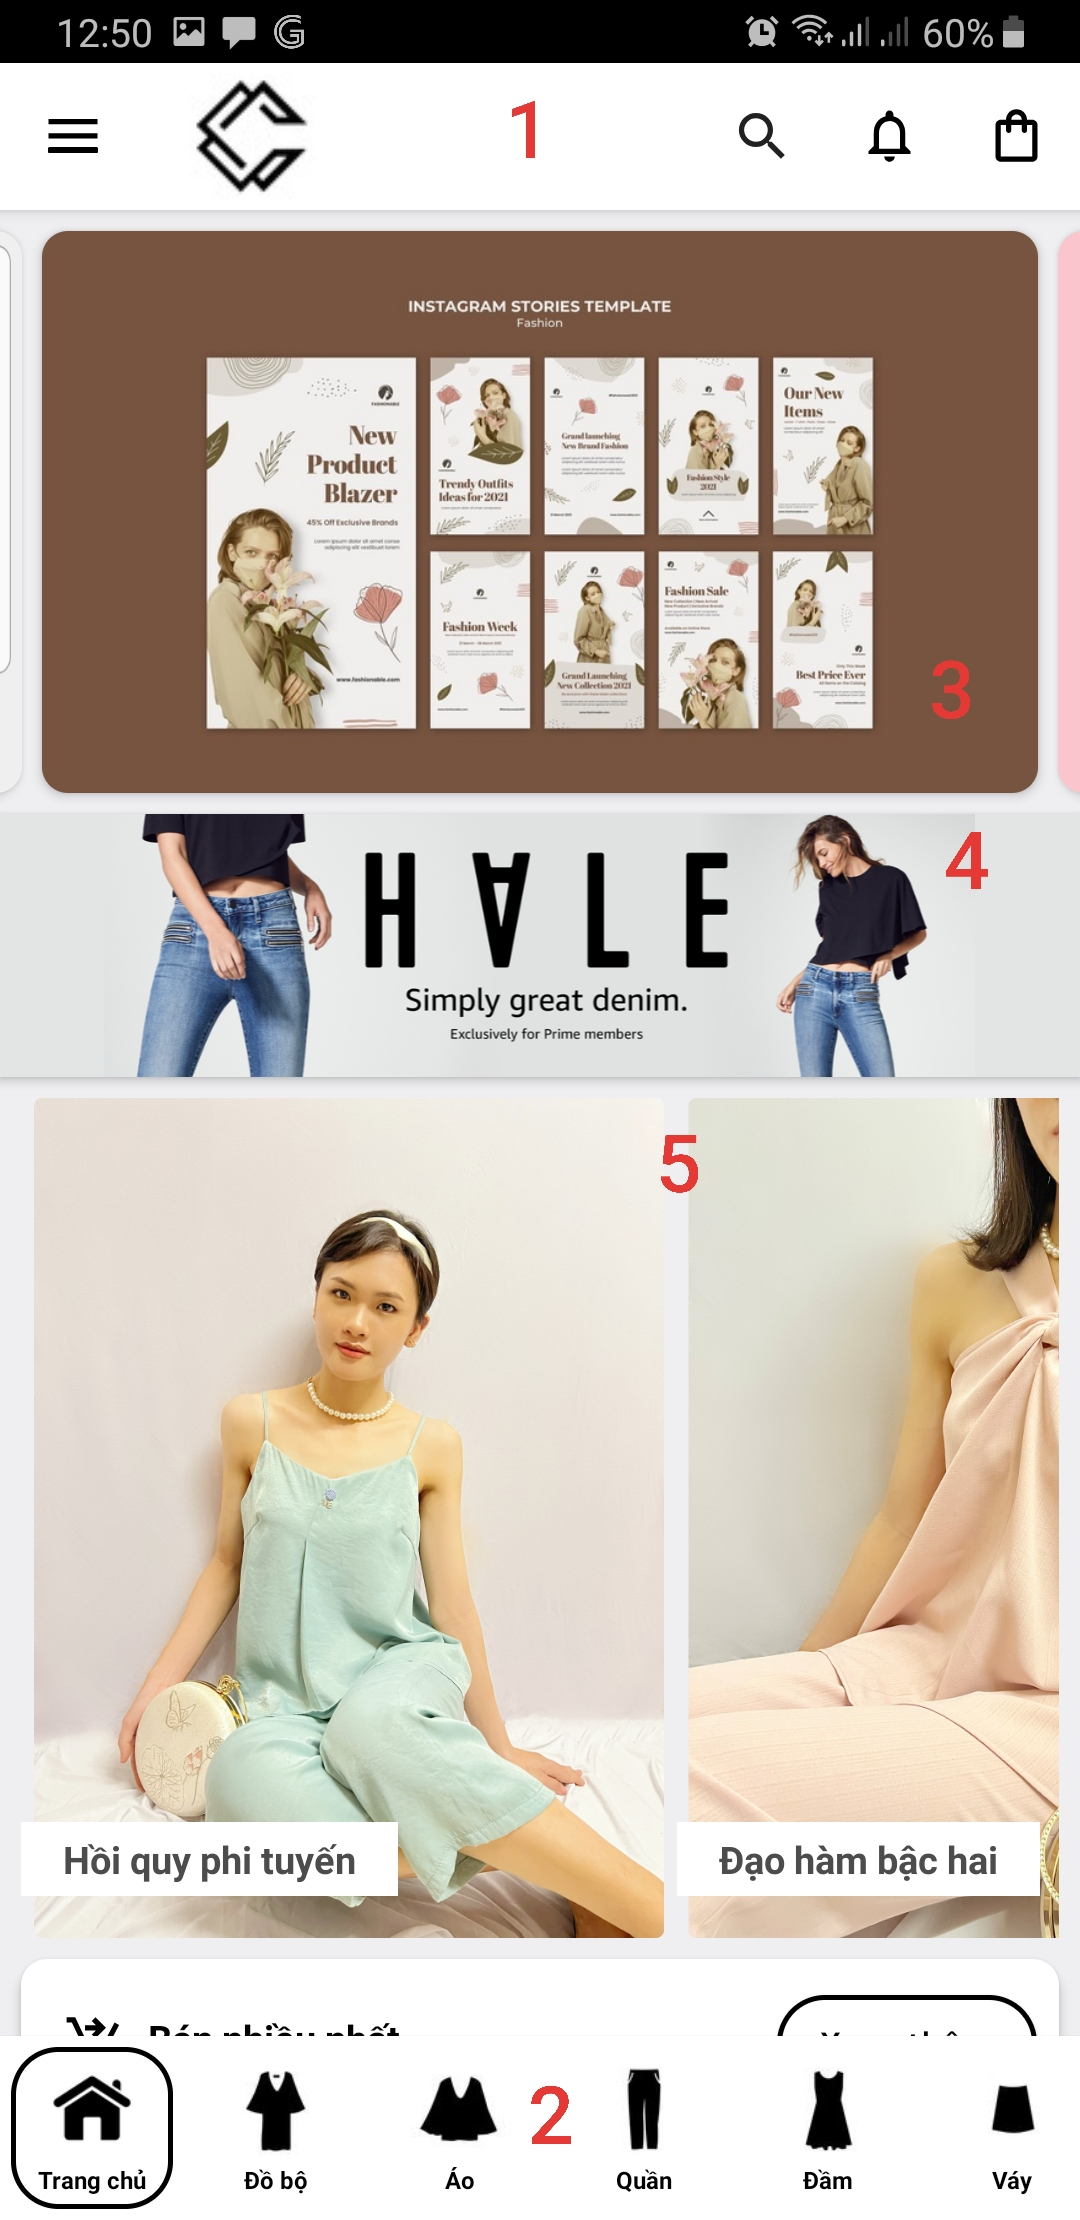
\includegraphics[height=0.7\textheight]{images/06.png}
            \caption{\centering\tiny{Hình 11: Màn hình chính của ứng dụng 1}}

        \end{figure}
        \column{0.7\linewidth}
        \indent \textbf{Các thành phần và chức năng kèm theo trên màn hình:}
        \begin{itemize}
            \item \textbf{2}: Horizontal Recycler View - hiển thị các sản phẩm theo danh mục.
            \item \textbf{3}: Carousel (View Pager) - hiển thị các chương trình, khuyến mãi của cửa hàng. Sau ba giây sẽ tự chuyển.
            \item \textbf{4}: Banner (Image View) - dùng để chèn quảng cáo.
            \item \textbf{5}: Slider (Horizontal Recycler View) - hiển thị các sản phẩm mới nhất.
        \end{itemize}
    \end{columns}
\end{frame}

% =========================================================================== Slide 12
\begin{frame}
    \begin{columns}
        \column{0.3\linewidth}
        \begin{figure}
            \centering
            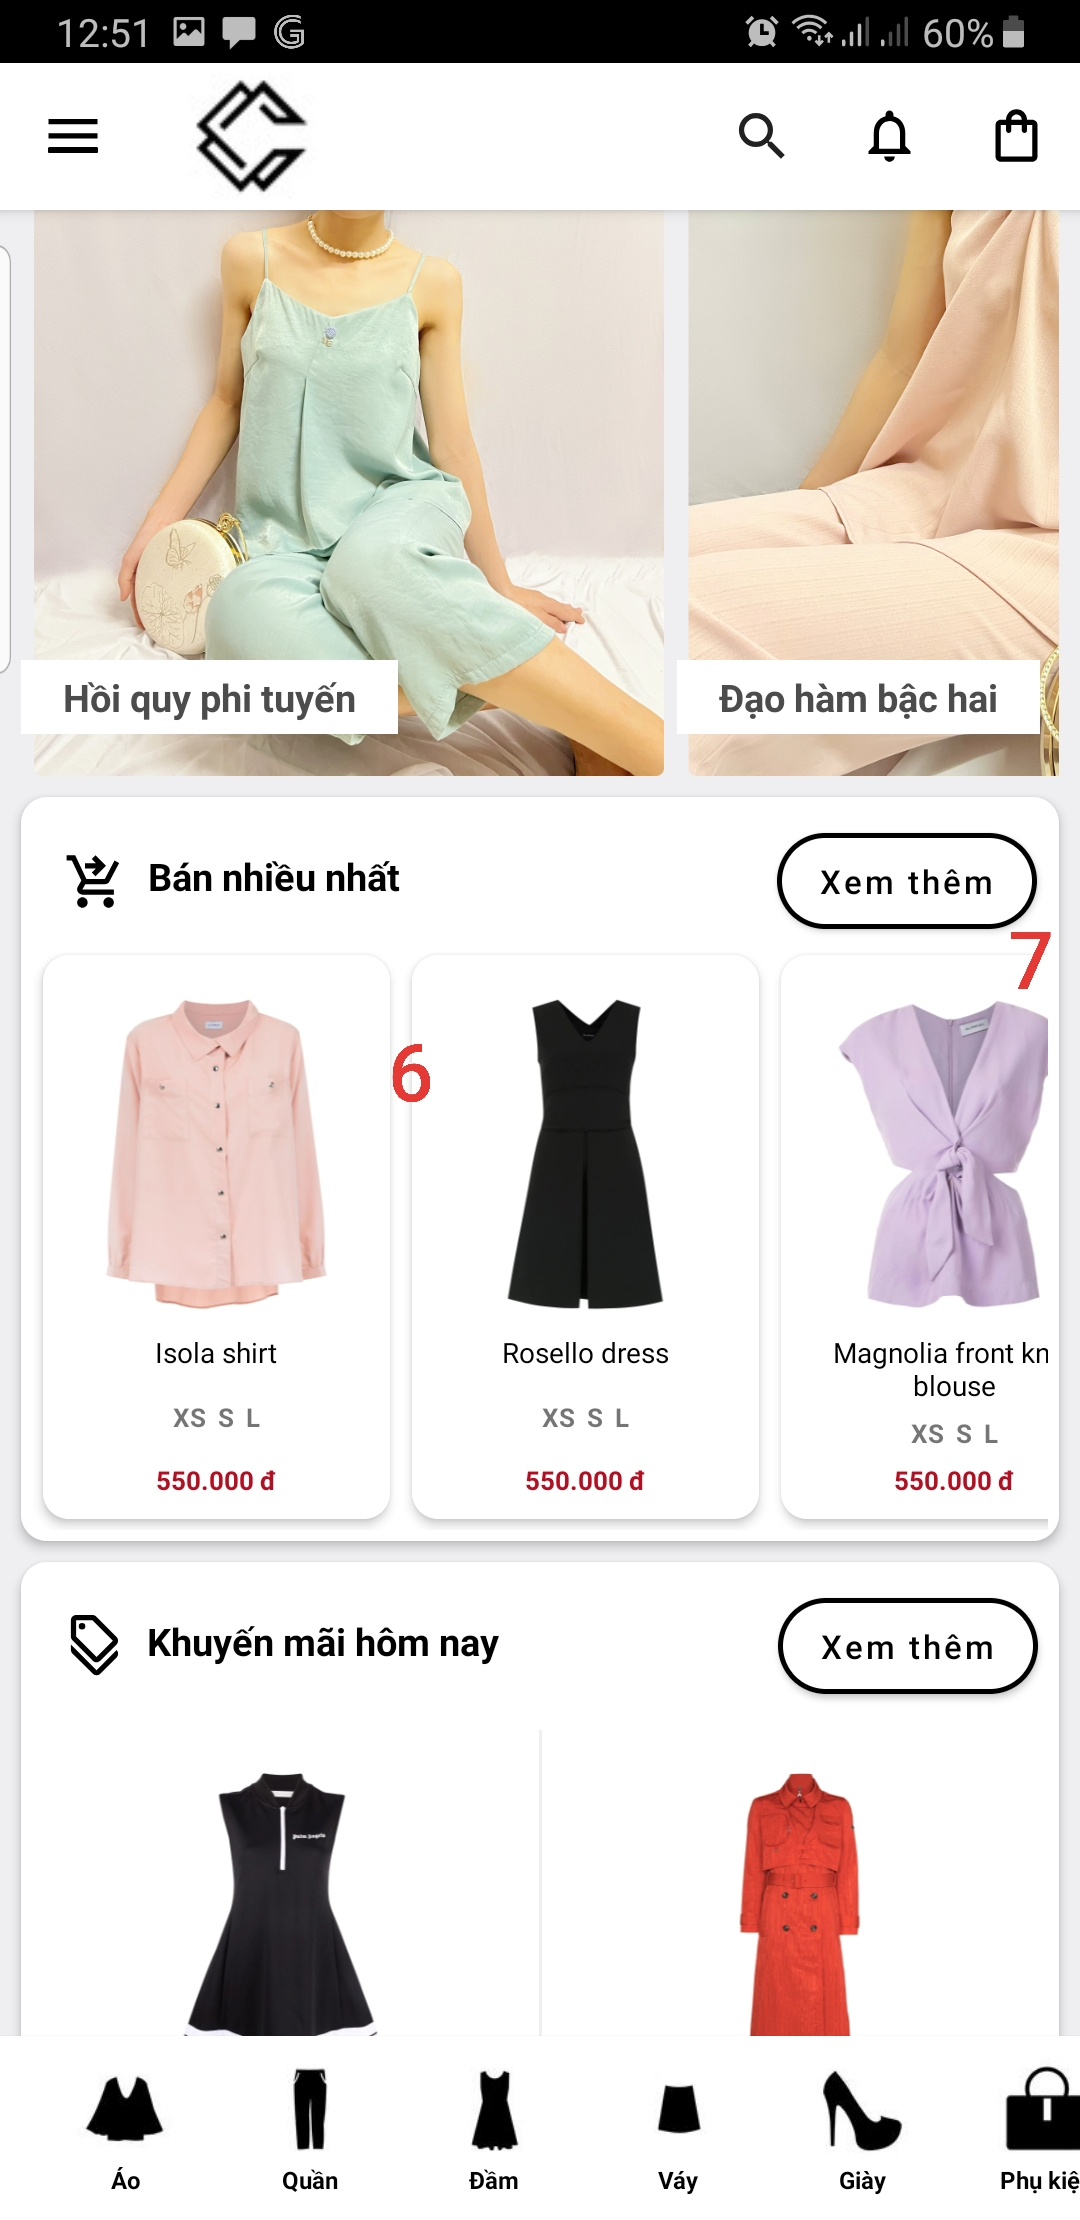
\includegraphics[height=0.7\textheight]{images/07.png}
            \caption{\centering\tiny{Hình 12: Màn hình chính của ứng dụng 2}}

        \end{figure}
        \column{0.7\linewidth}
        \indent \textbf{Các thành phần và chức năng kèm theo trên màn hình:}
        \begin{itemize}
            \item \textbf{6}: Horizontal Recycler View - hiển thị tám các sản phẩm bán chạy hiện tại. Nhấn vào item sẽ đưa đến trang chi tiết sản phẩm tương ứng.
            \item \textbf{7}: Button - đưa đến một fragment khác hiển thị nhiều hơn tám sản phẩm bán chạy dưới dạng GridView.
        \end{itemize}
    \end{columns}
\end{frame}

% =========================================================================== Slide 12
\begin{frame}
    \begin{columns}
        \column{0.3\linewidth}
        \begin{figure}
            \centering
            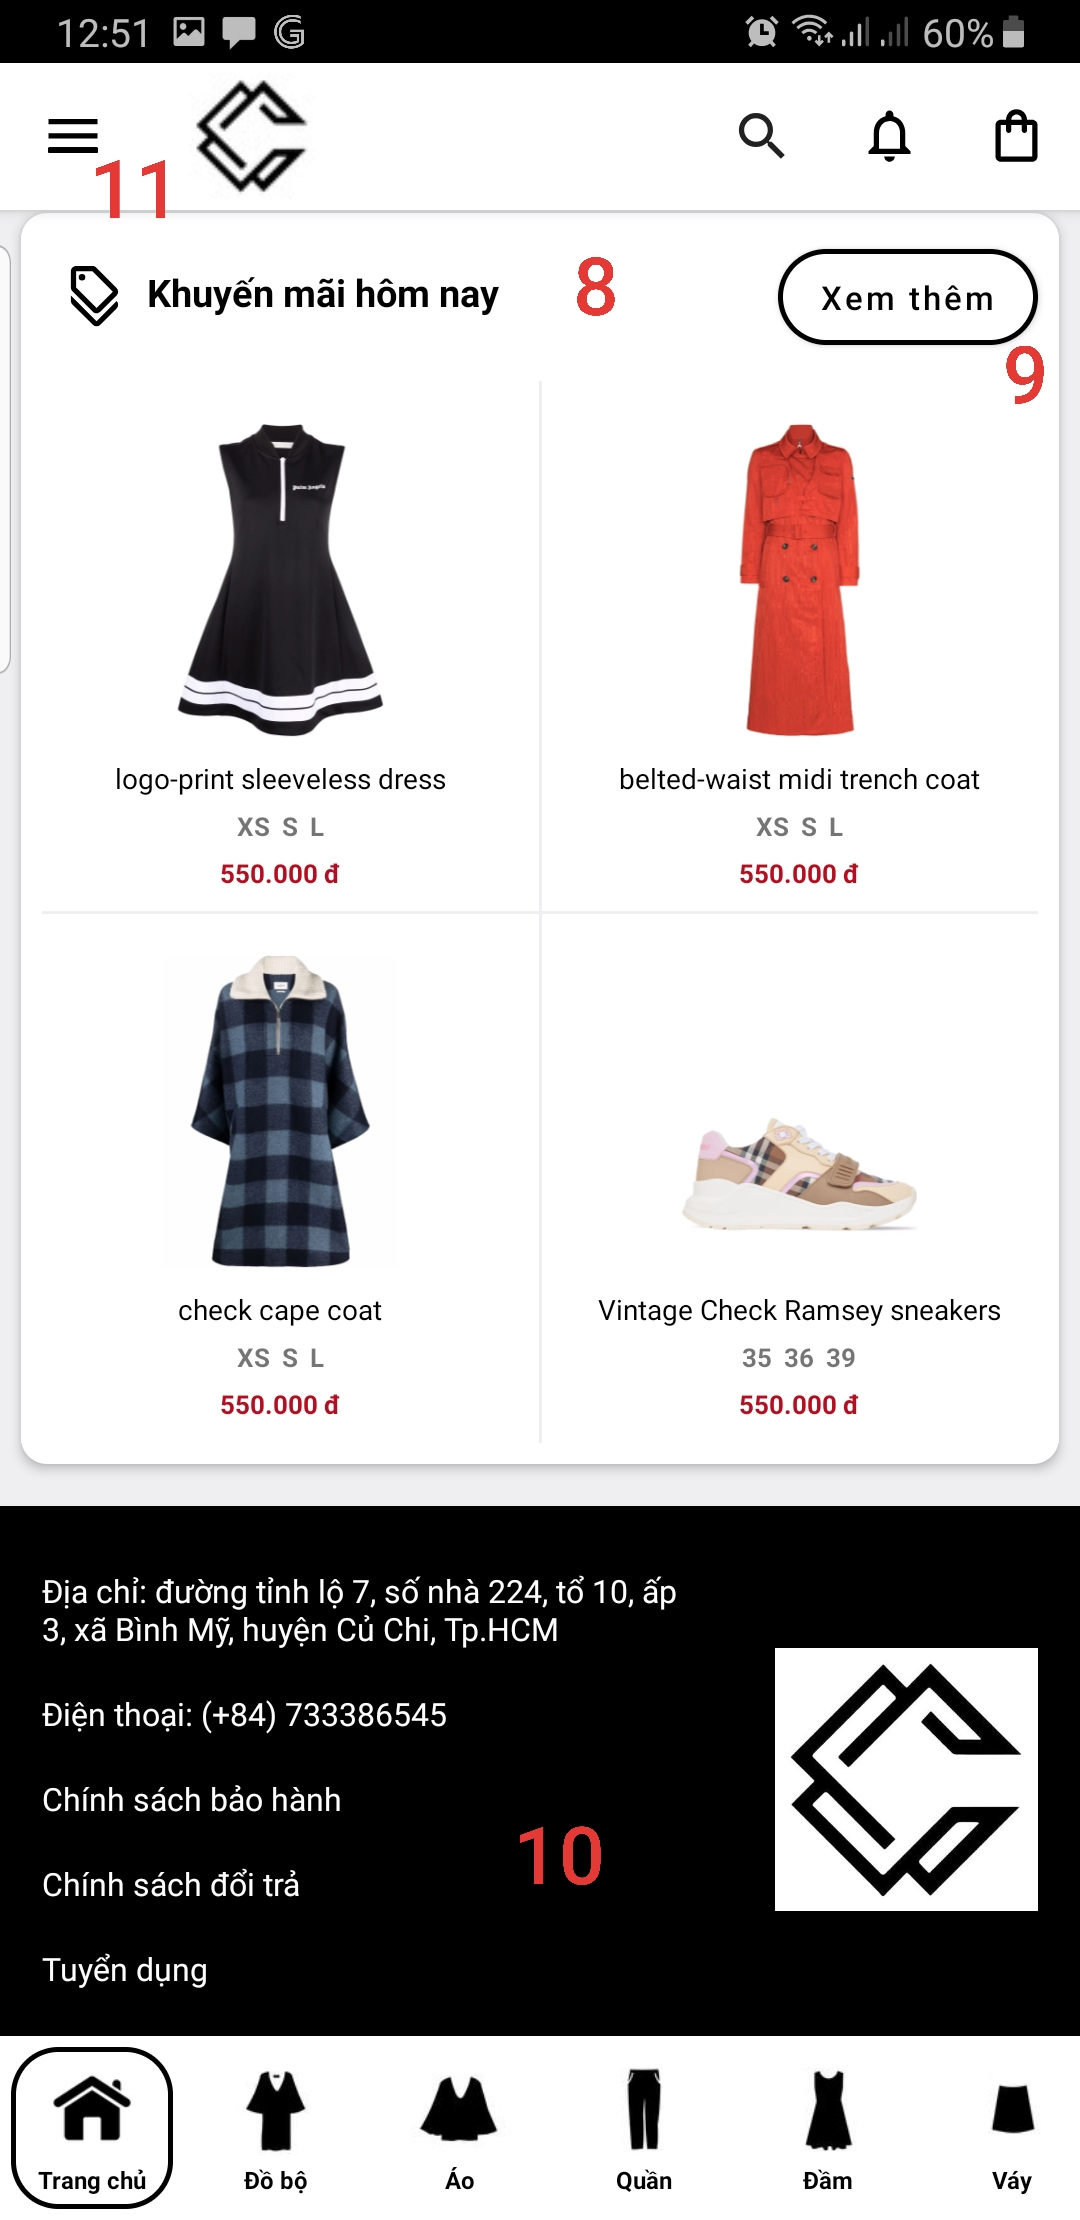
\includegraphics[height=0.7\textheight]{images/08.png}
            \caption{\centering\tiny{Hình 13: Màn hình chính của ứng dụng 3}}

        \end{figure}
        \column{0.7\linewidth}
        \indent \textbf{Các thành phần và chức năng kèm theo trên màn hình:}
        \begin{itemize}
            \item \textbf{8}: GridView - hiển thị bốn sản phẩm được khuyến mãi hôm nay. Nhấn vào item sẽ đứa đến trang chi tiết sản phẩm tương ứng.
            \item \textbf{9}: Button - nhấn vào sẽ đưa đến một fragment khác hiển thị nhiều sản phẩm khuyến mãi hơn dưới dạng GridView.
            \item \textbf{10}: Footer - thể hiện địa chỉ, số điện thoại, các chính sách đổi trả, bảo hành của nhãn hàng.
            \item \textbf{11}: Hamburger toggle - nhấn vào để mở navigation view.
        \end{itemize}
    \end{columns}
\end{frame}

\begin{frame}
    \frametitle{Các màn hình và chức năng kèm theo (7)}
    \framesubtitle{Màn hình chính - Mã nguồn minh họa}

    \begin{columns}
        \column{0.3\linewidth}
        \begin{figure}
            \centering
            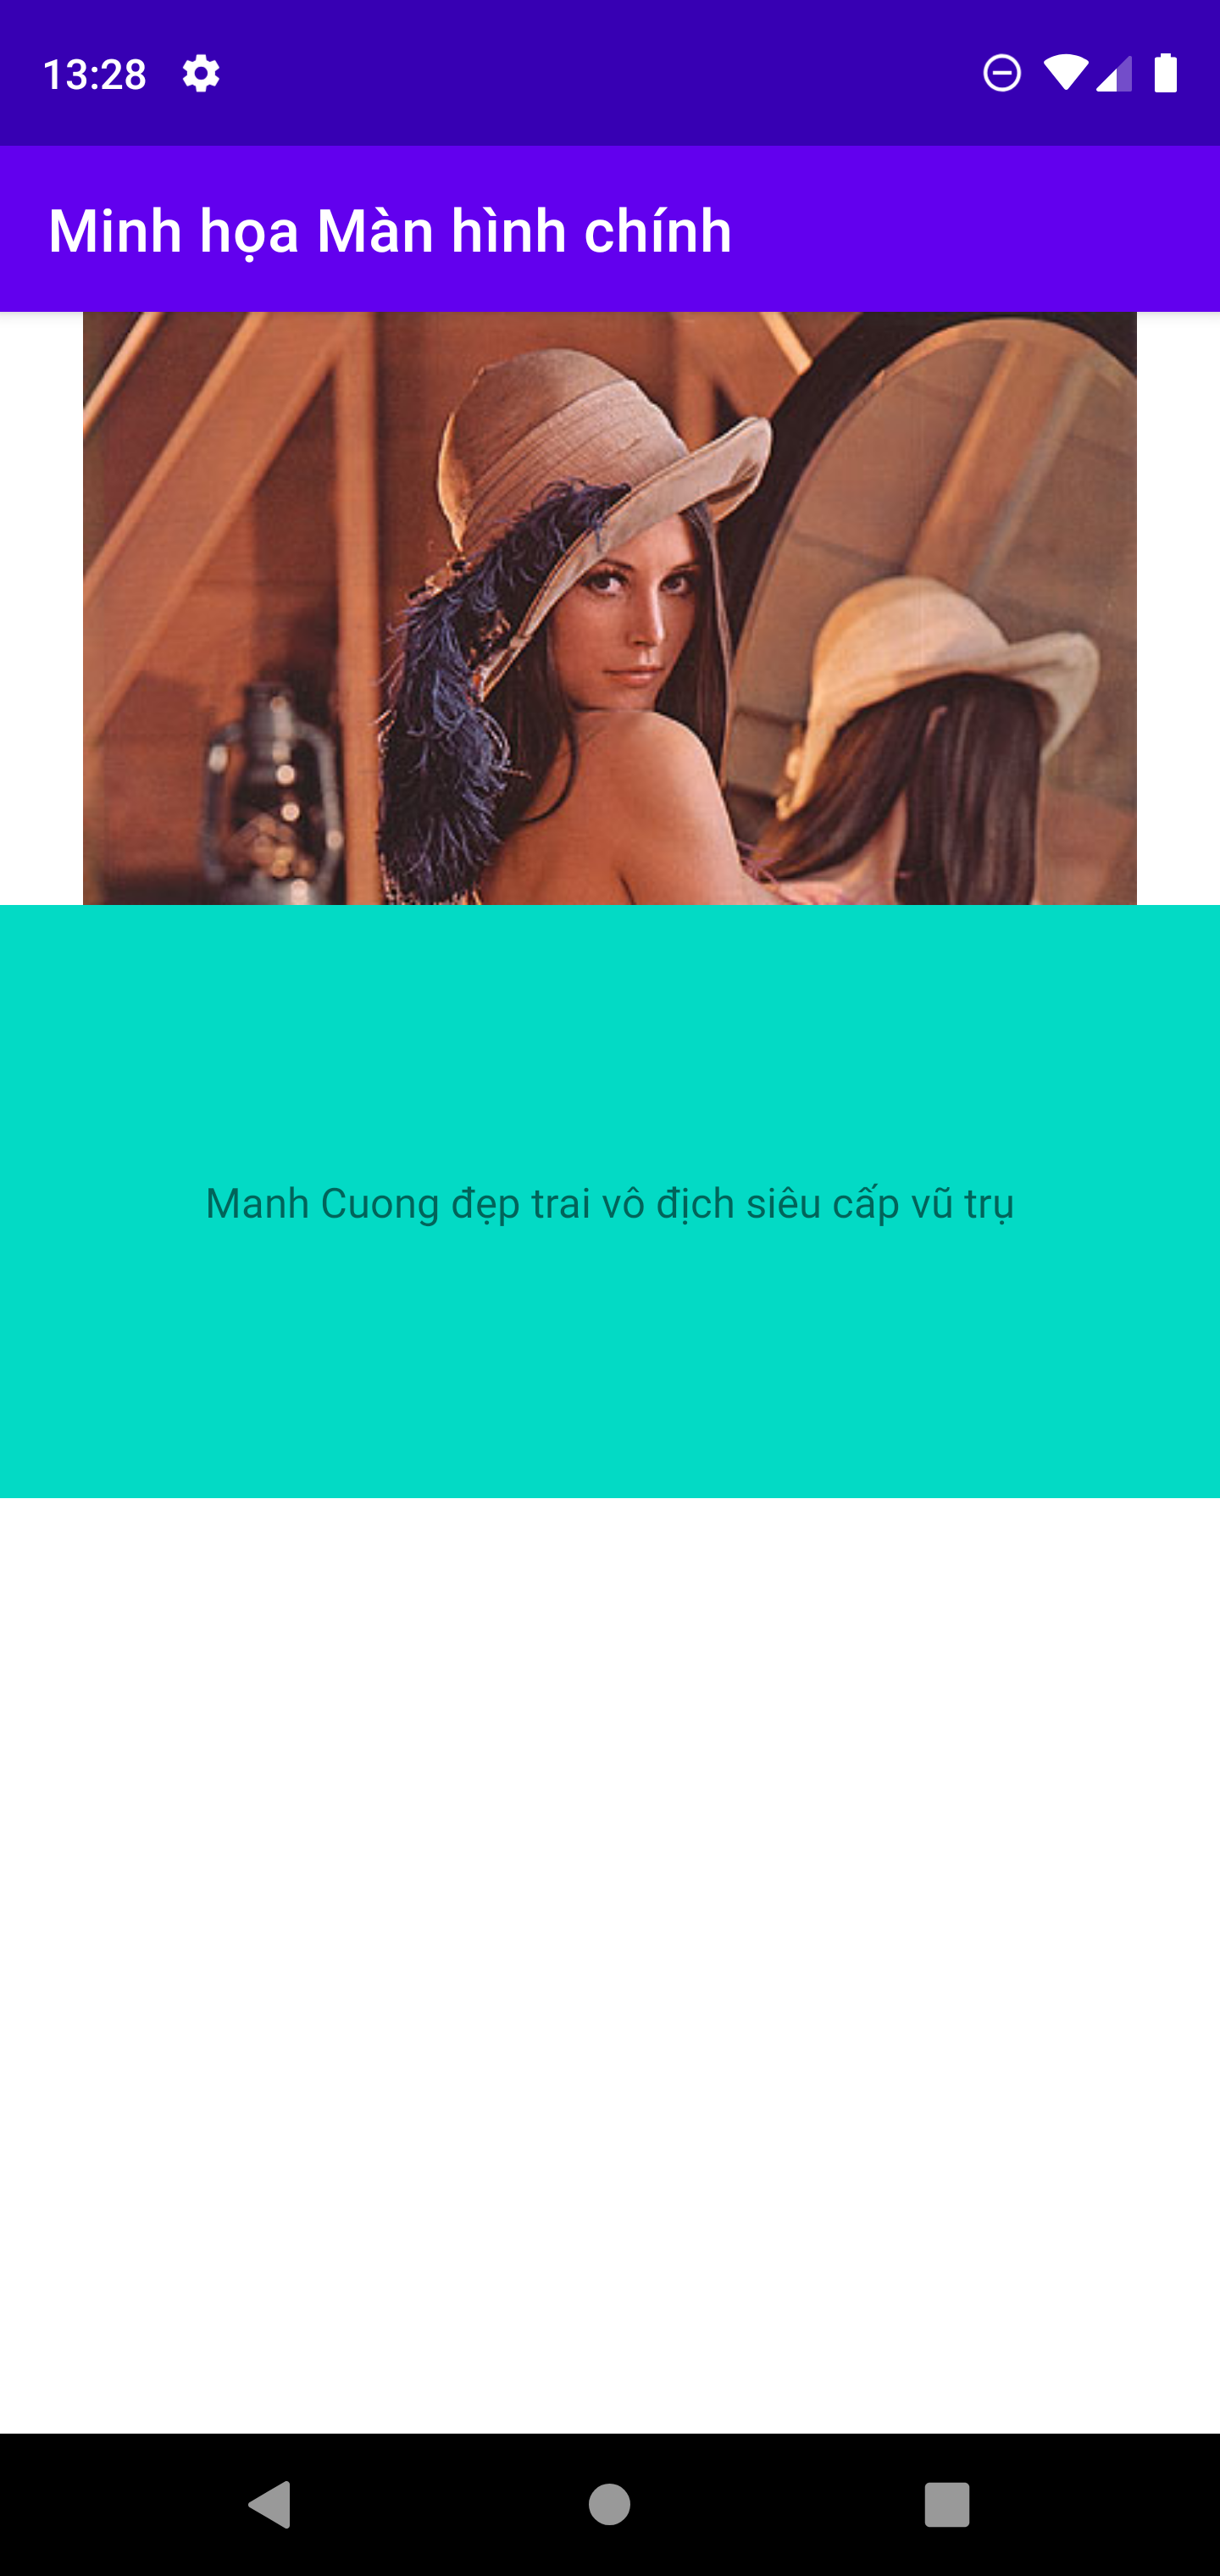
\includegraphics[height=0.7\textheight]{images/10.png}
            \caption{\centering\tiny{Hình 14: Minh họa màn hình chính của ứng dụng}}
        \end{figure}
        \column{0.7\linewidth}
        \indent Cấu trúc cây thư mục:
        \begin{figure}
            \centering
            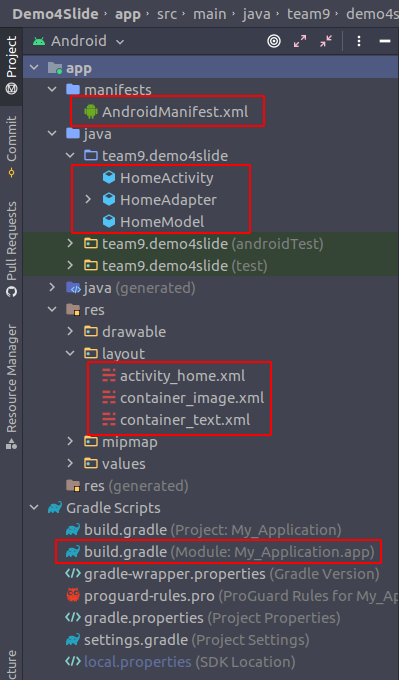
\includegraphics[height=0.68\textheight]{images/11.png}
        \end{figure}
    \end{columns}
\end{frame}

\begin{frame}
    \begin{columns}
        \column{0.3\linewidth}
        \begin{figure}
            \centering
            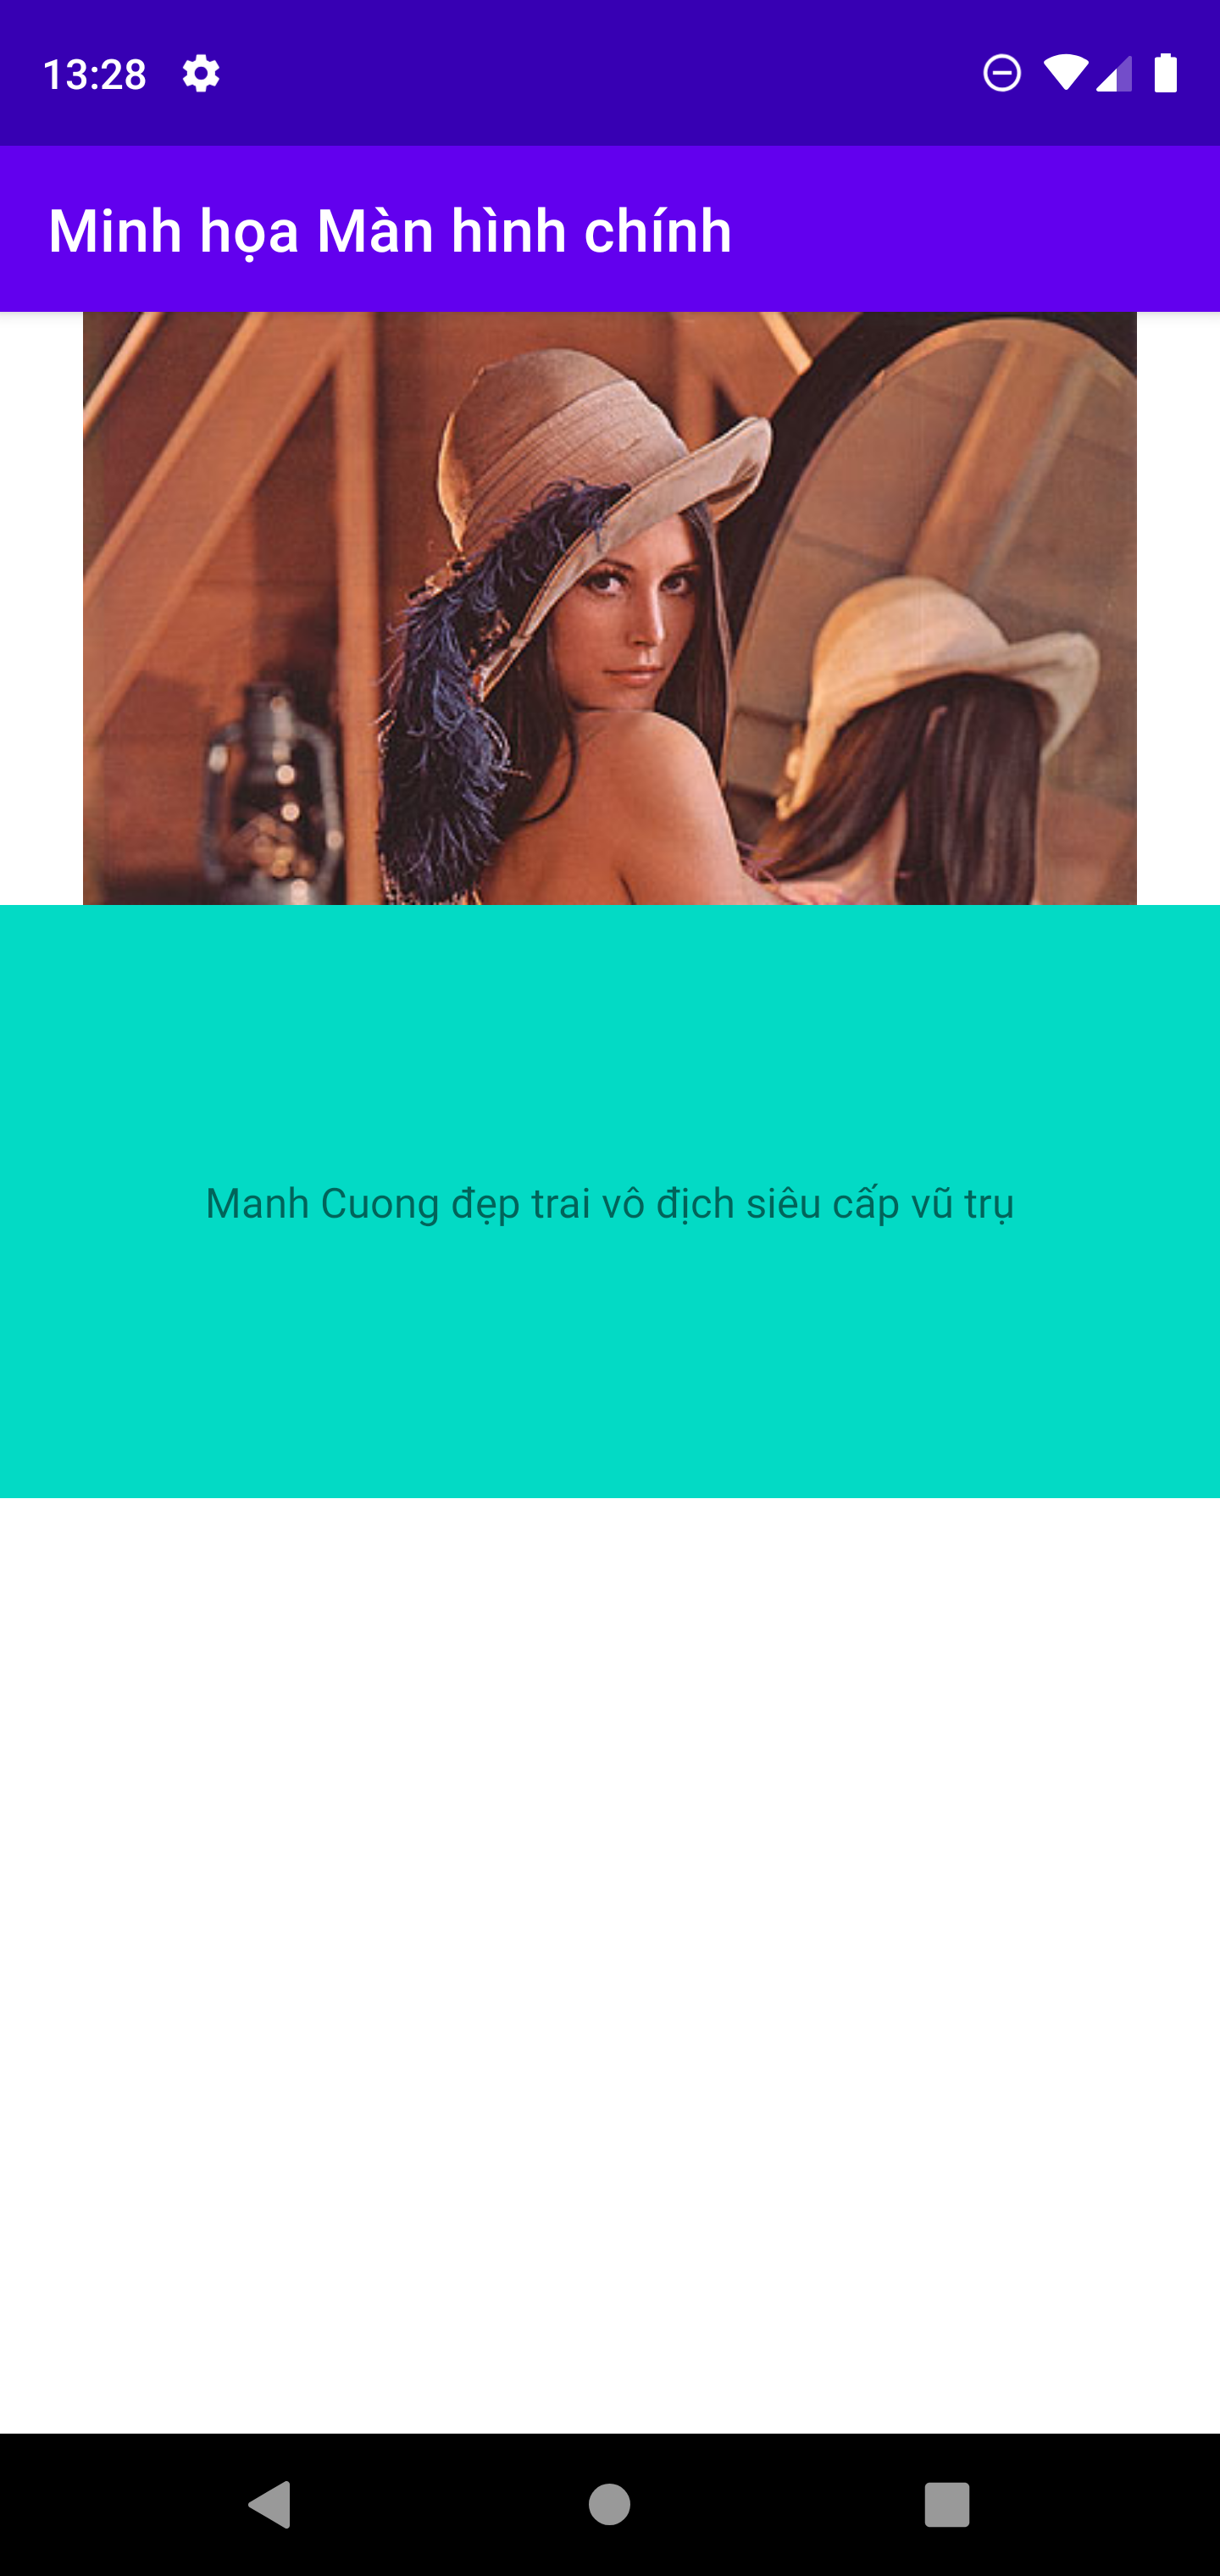
\includegraphics[height=0.7\textheight]{images/10.png}
            \caption{\centering\tiny{Hình 14: Minh họa màn hình chính của ứng dụng}}
        \end{figure}
        \column{0.7\linewidth}
        \indent \textbf{\texttt{AndroidManifest.xml}}
        \begin{figure}
            \centering
            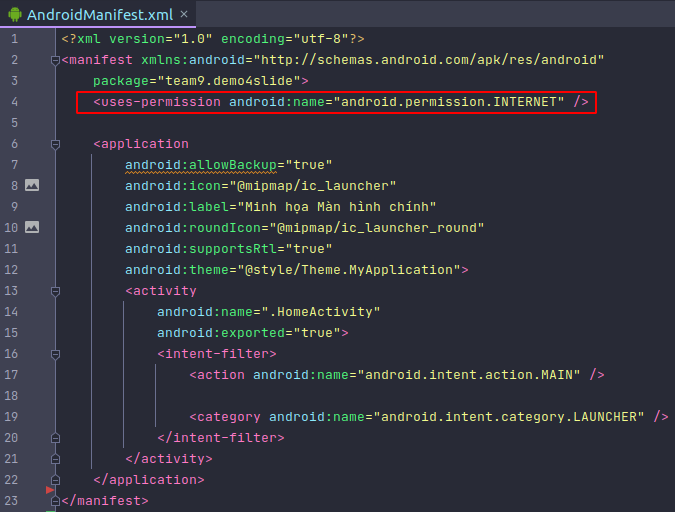
\includegraphics[width=\textwidth]{images/12.png}
        \end{figure}
    \end{columns}
\end{frame}

\begin{frame}
    \begin{columns}
        \column{0.3\linewidth}
        \begin{figure}
            \centering
            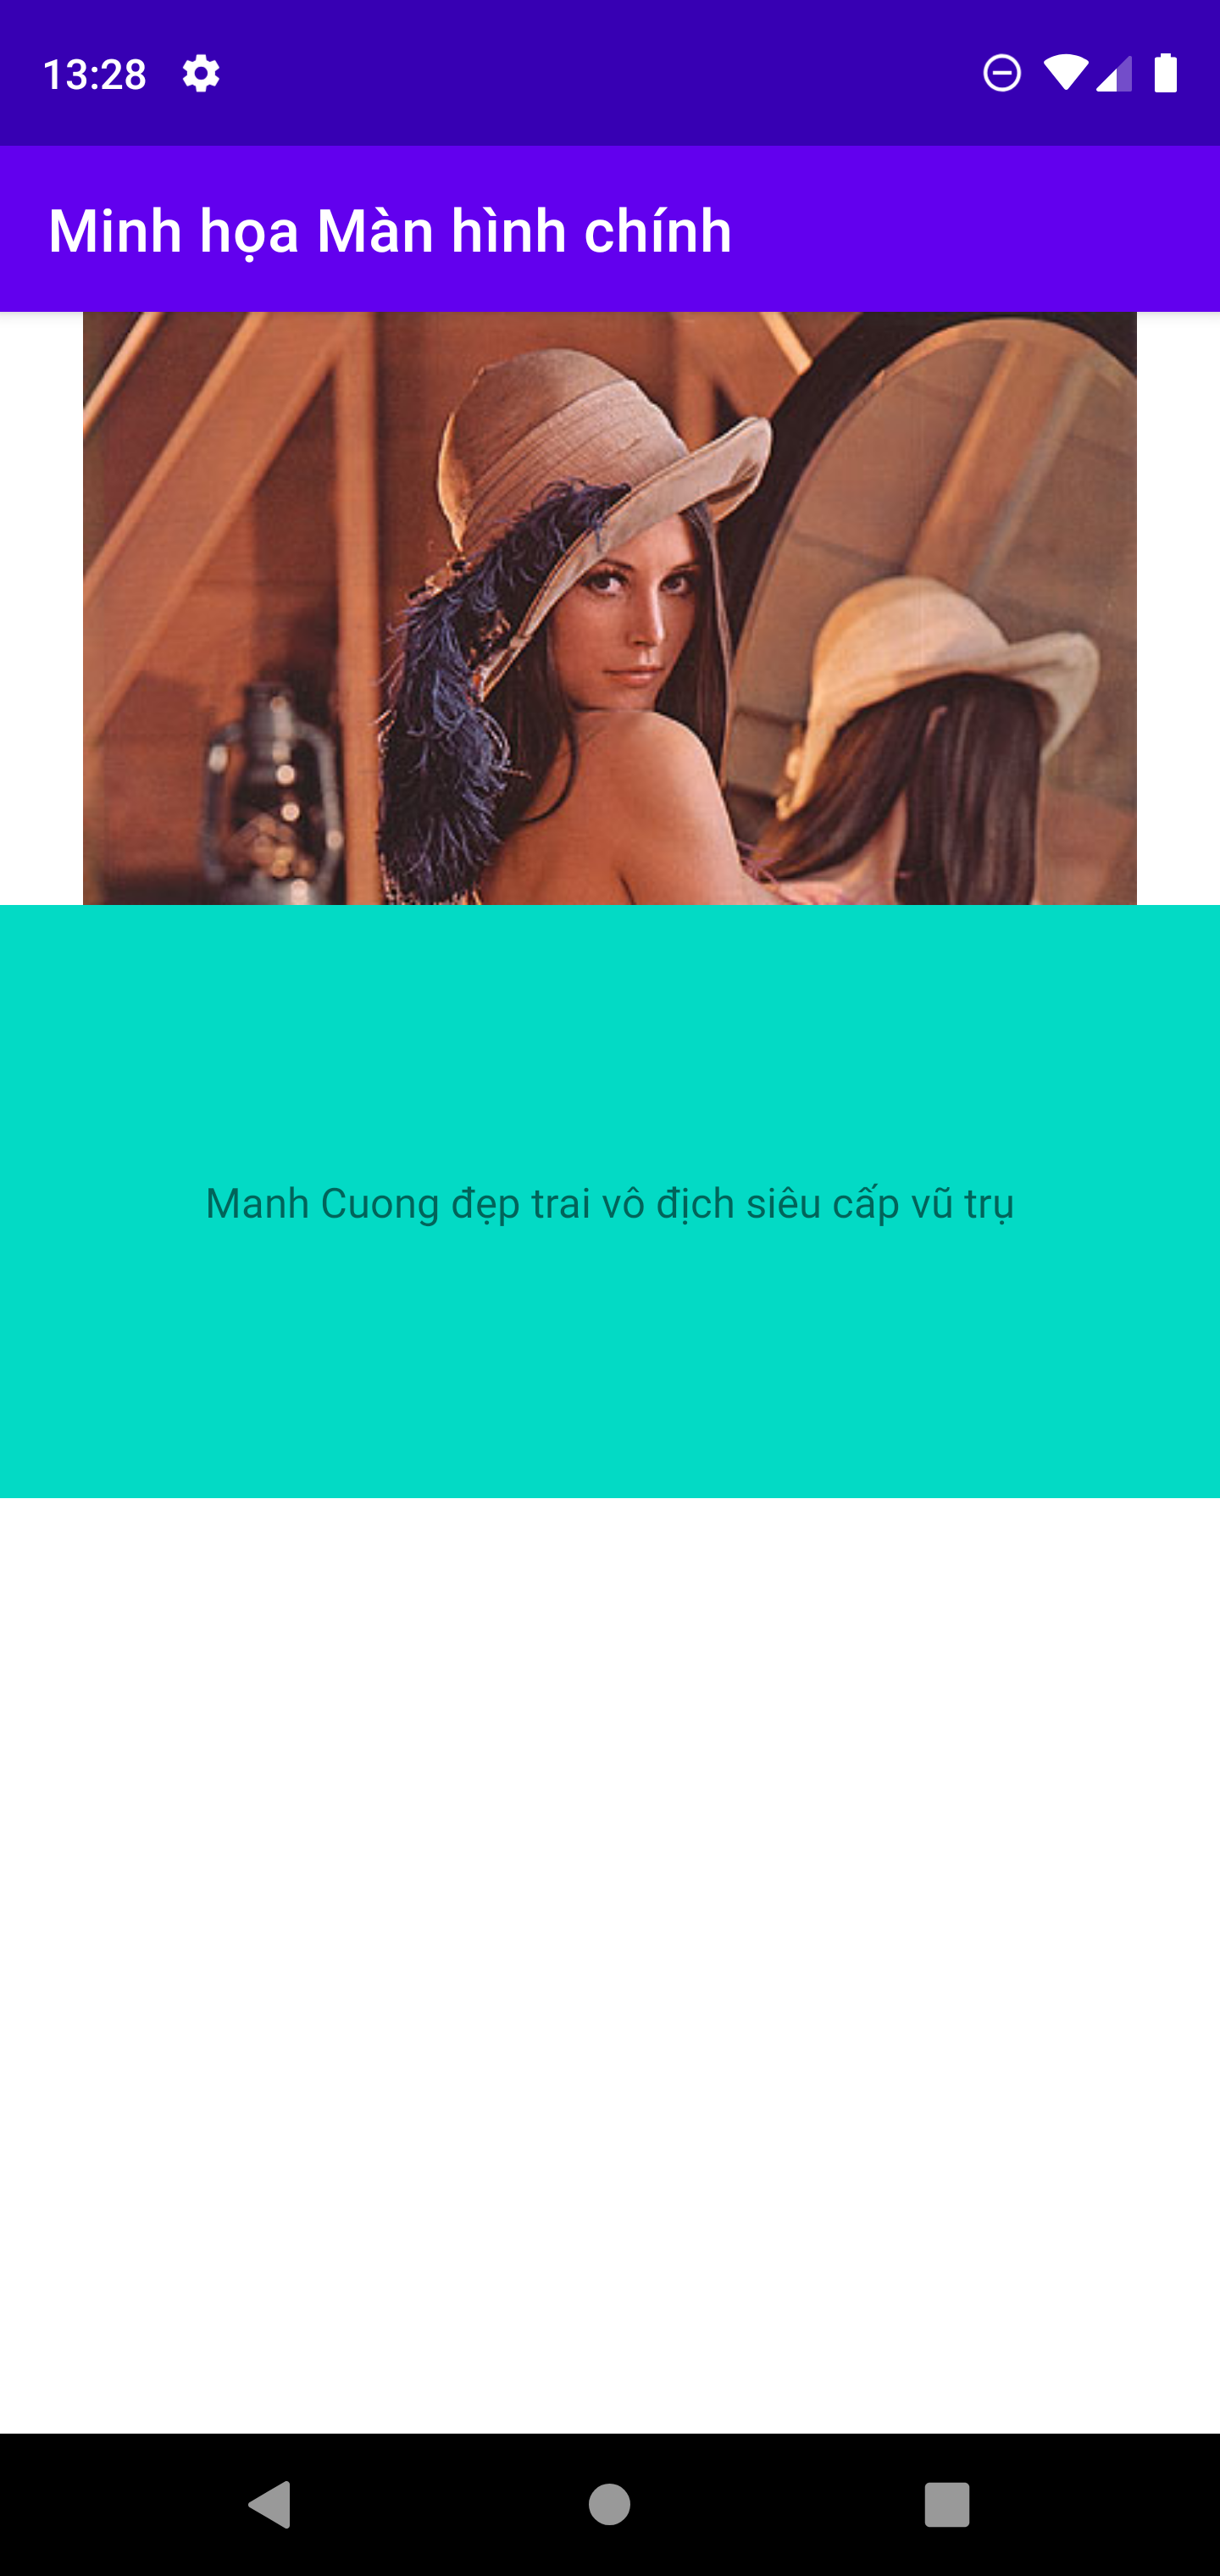
\includegraphics[height=0.7\textheight]{images/10.png}
            \caption{\centering\tiny{Hình 14: Minh họa màn hình chính của ứng dụng}}
        \end{figure}
        \column{0.7\linewidth}
        \indent \textbf{\texttt{build.gradle}}
        \begin{figure}
            \centering
            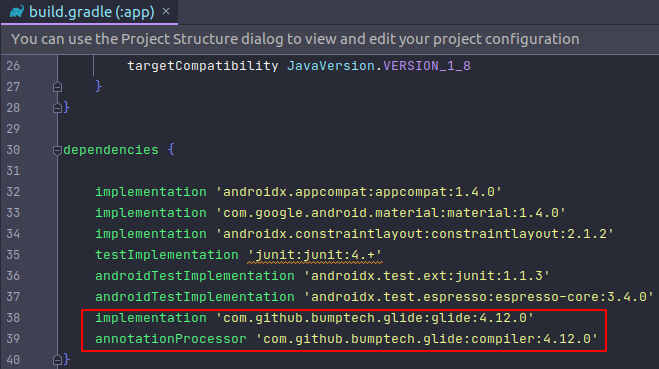
\includegraphics[width=\textwidth]{images/13.png}
        \end{figure}
    \end{columns}
\end{frame}

\begin{frame}
    \begin{columns}
        \column{0.3\linewidth}
        \begin{figure}
            \centering
            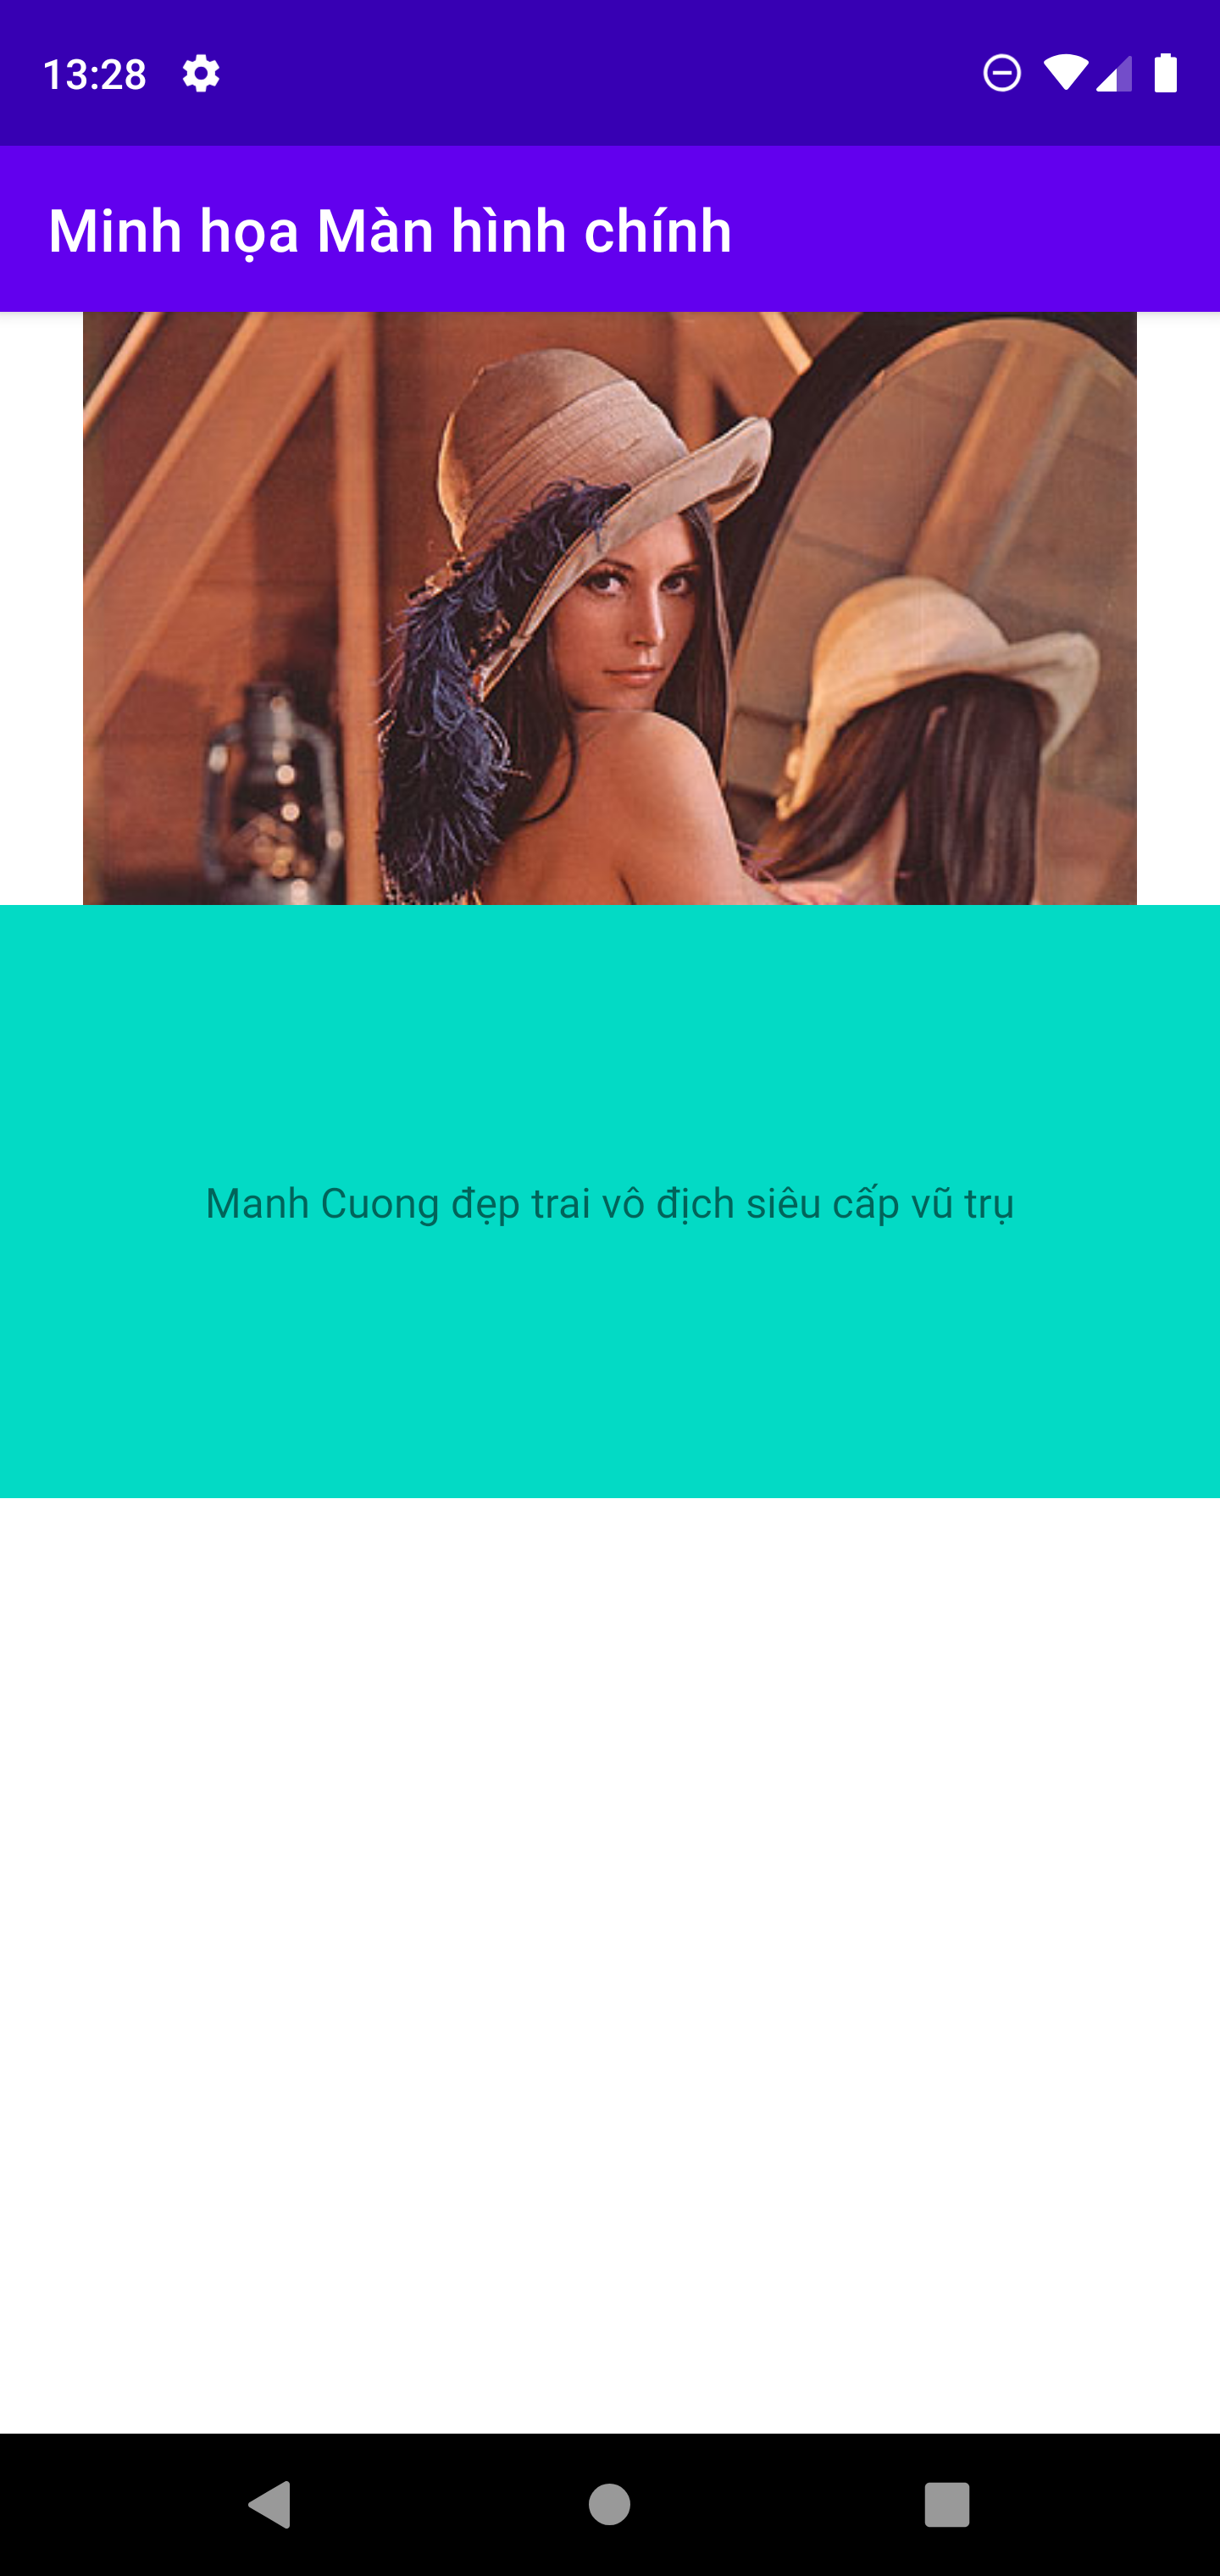
\includegraphics[height=0.7\textheight]{images/10.png}
            \caption{\centering\tiny{Hình 14: Minh họa màn hình chính của ứng dụng}}
        \end{figure}
        \column{0.7\linewidth}
        \indent \textbf{\texttt{activity\_home.xml}}
        \begin{figure}
            \centering
            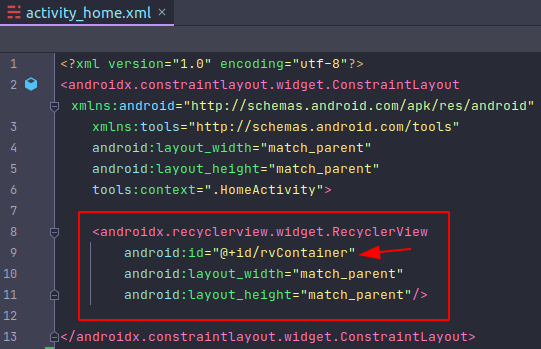
\includegraphics[width=\textwidth]{images/14.png}
        \end{figure}
    \end{columns}
\end{frame}

\begin{frame}
    \begin{columns}
        \column{0.3\linewidth}
        \begin{figure}
            \centering
            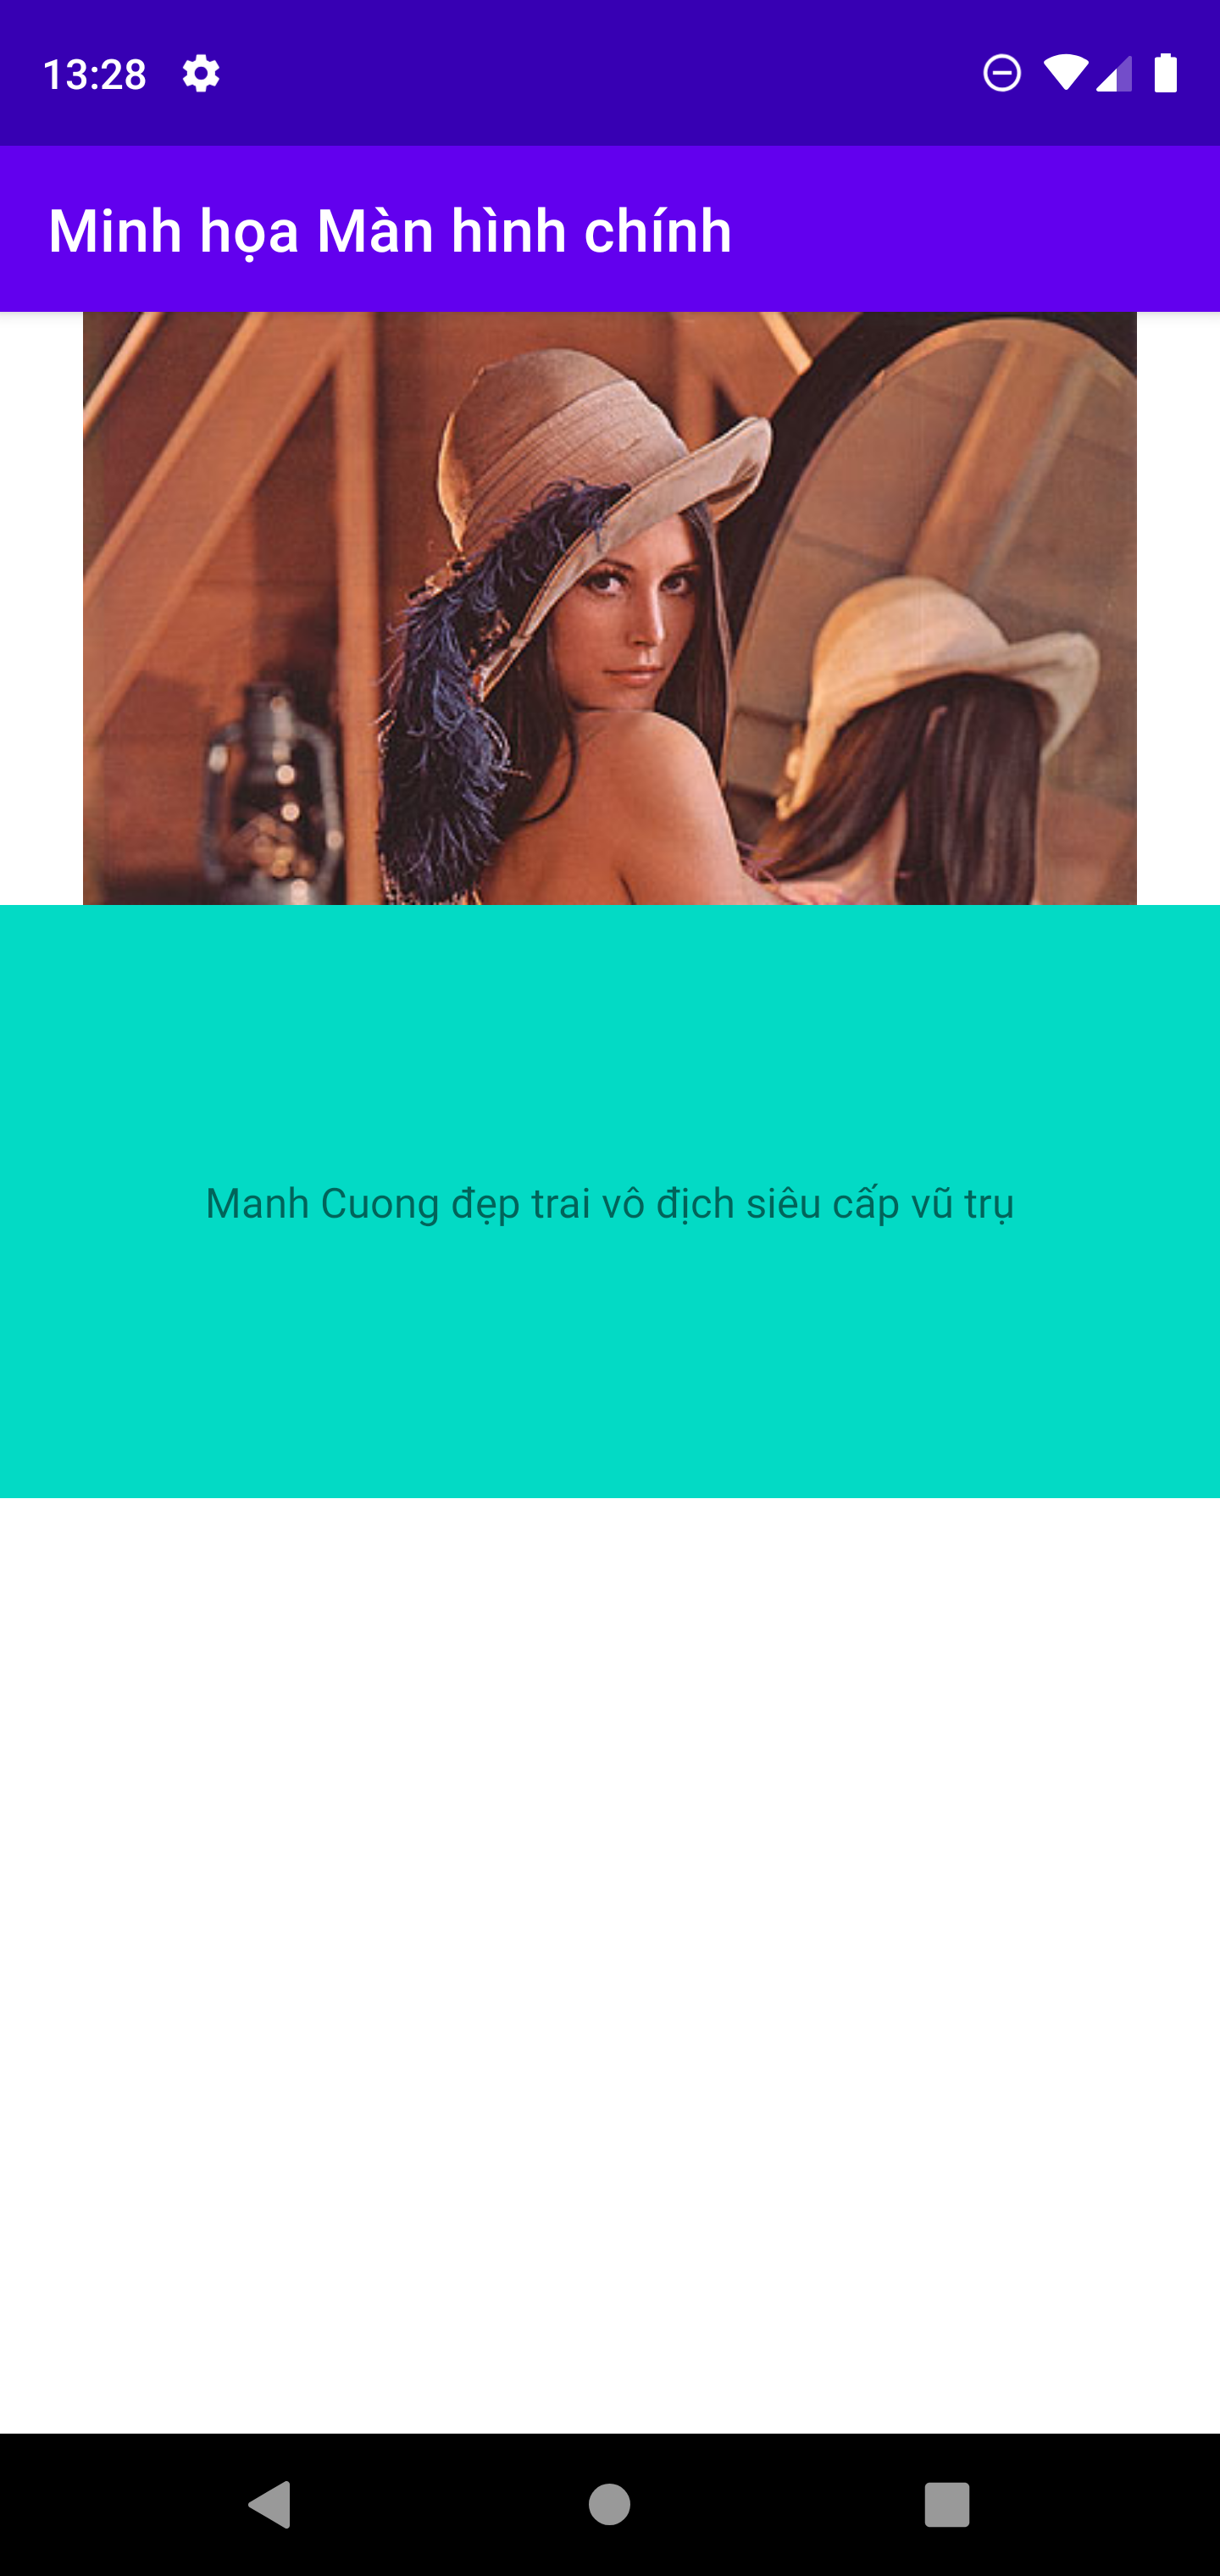
\includegraphics[height=0.7\textheight]{images/10.png}
            \caption{\centering\tiny{Hình 14: Minh họa màn hình chính của ứng dụng}}
        \end{figure}
        \column{0.7\linewidth}
        \indent \textbf{\texttt{container\_image.xml}}
        \begin{figure}
            \centering
            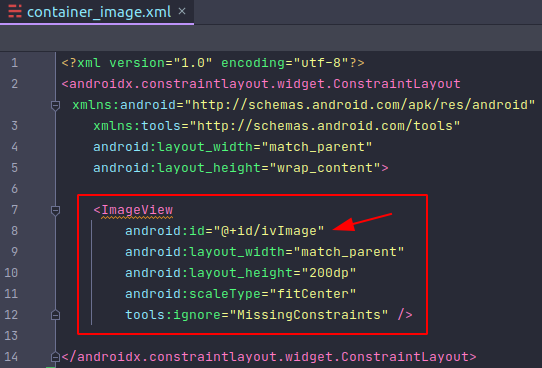
\includegraphics[width=\textwidth]{images/15.png}
        \end{figure}
    \end{columns}
\end{frame}

\begin{frame}
    \begin{columns}
        \column{0.3\linewidth}
        \begin{figure}
            \centering
            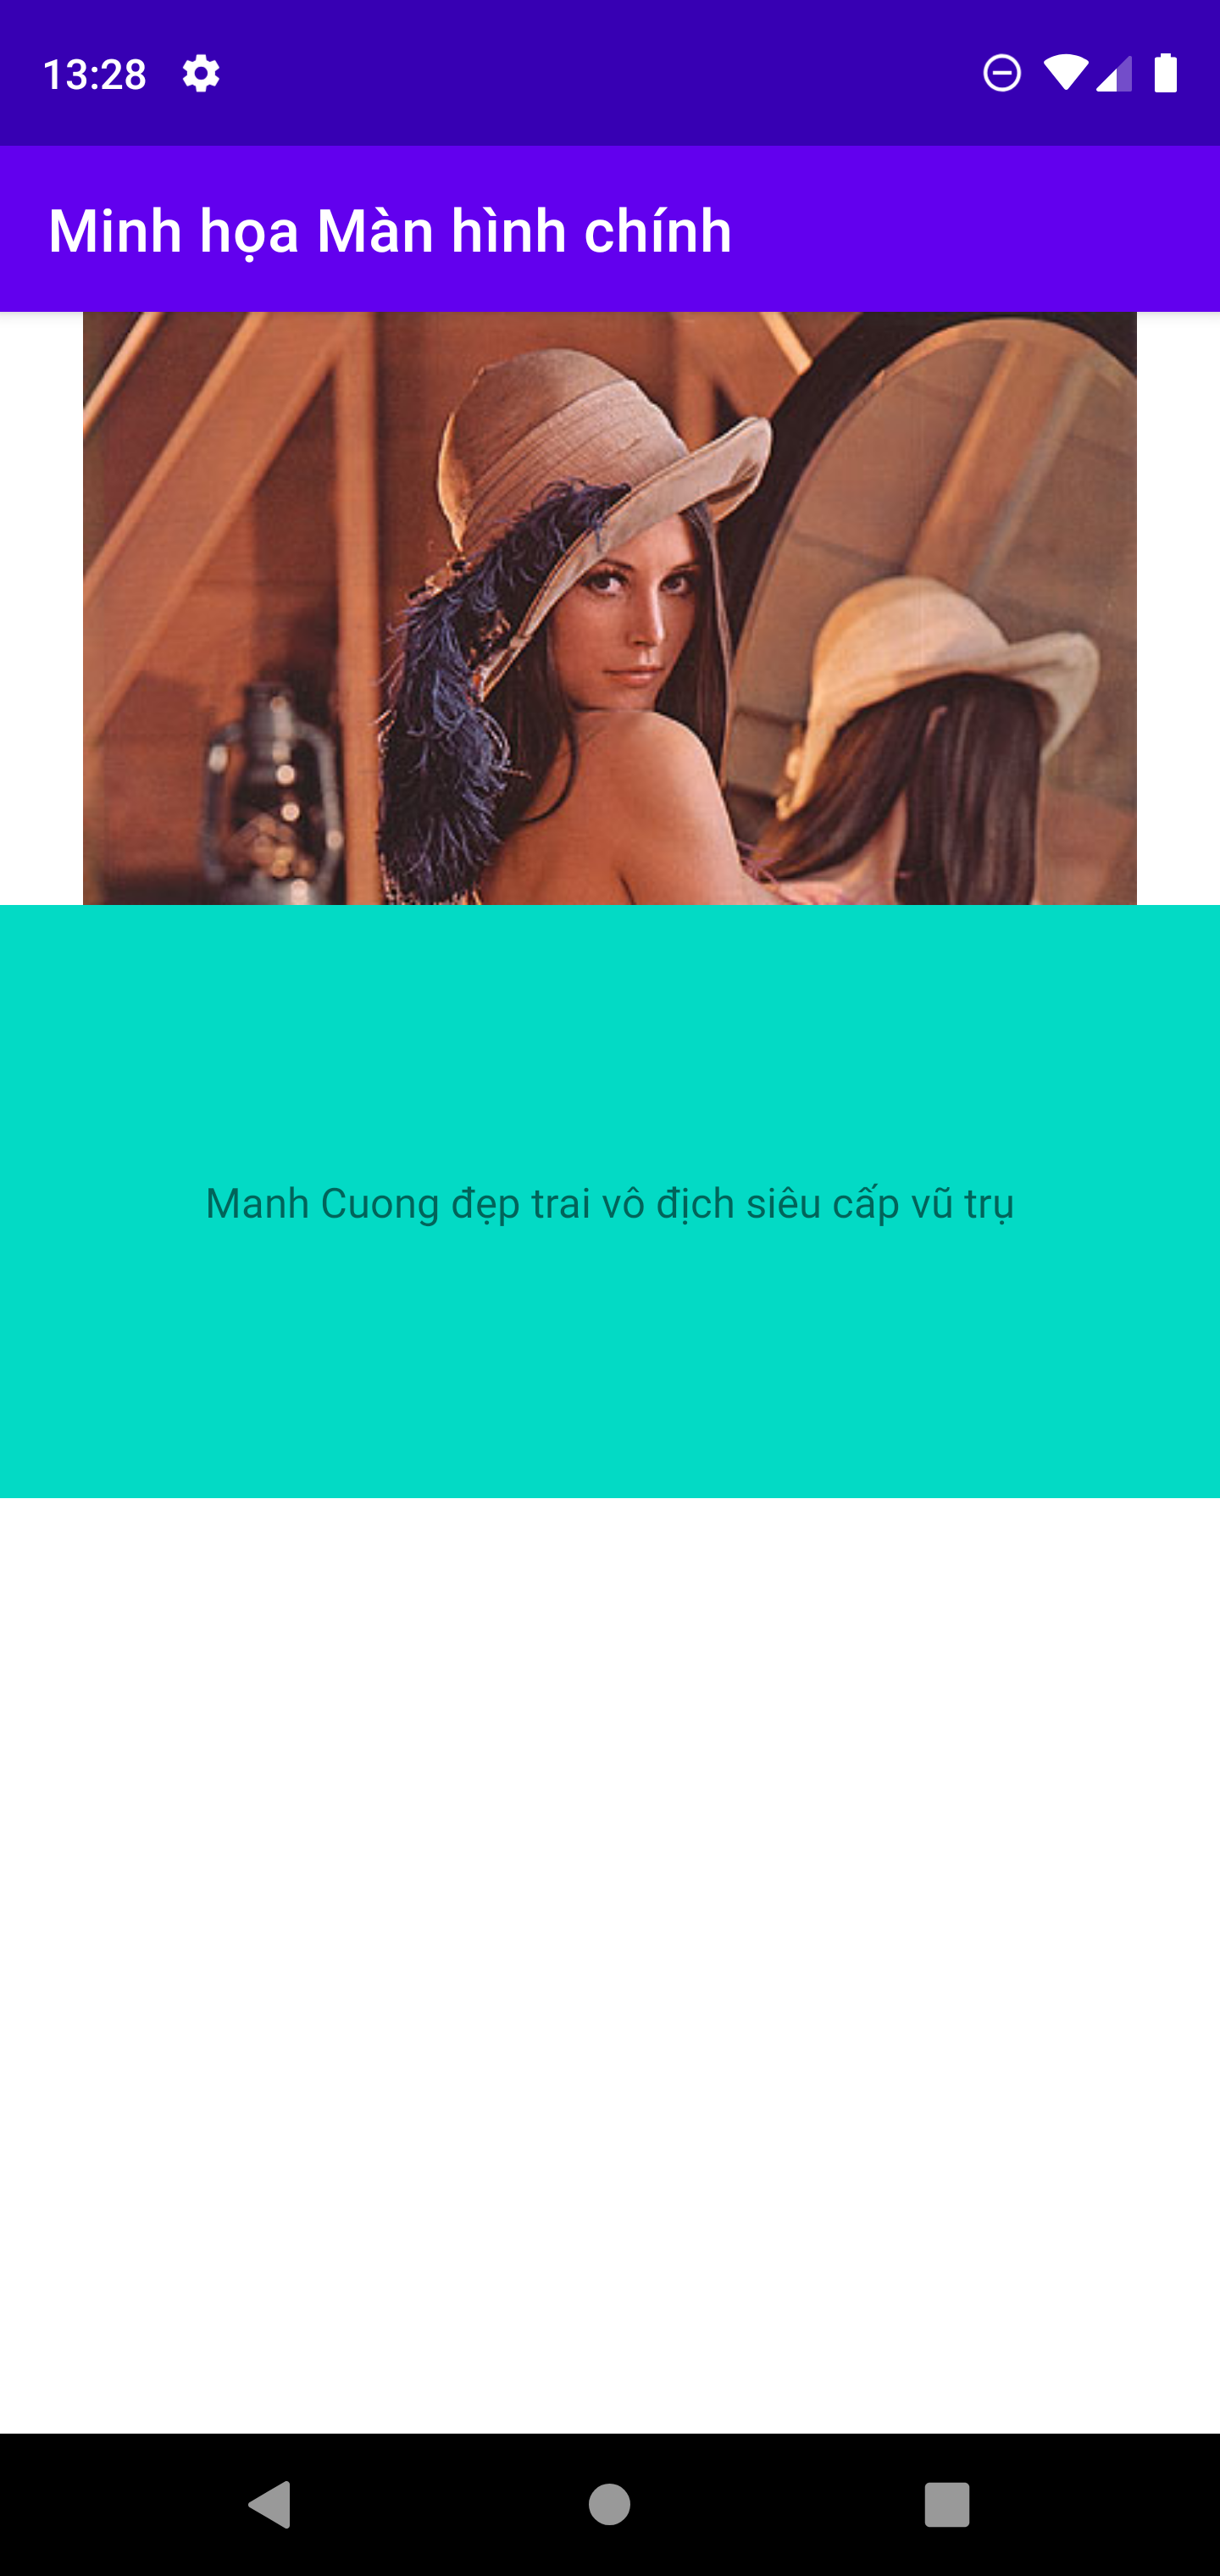
\includegraphics[height=0.7\textheight]{images/10.png}
            \caption{\centering\tiny{Hình 14: Minh họa màn hình chính của ứng dụng}}
        \end{figure}
        \column{0.7\linewidth}
        \indent \textbf{\texttt{container\_text.xml}}
        \begin{figure}
            \centering
            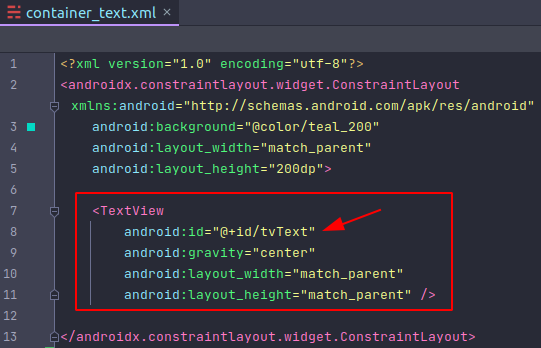
\includegraphics[width=\textwidth]{images/16.png}
        \end{figure}
    \end{columns}
\end{frame}

\begin{frame}
    \begin{columns}
        \column{0.3\linewidth}
        \begin{figure}
            \centering
            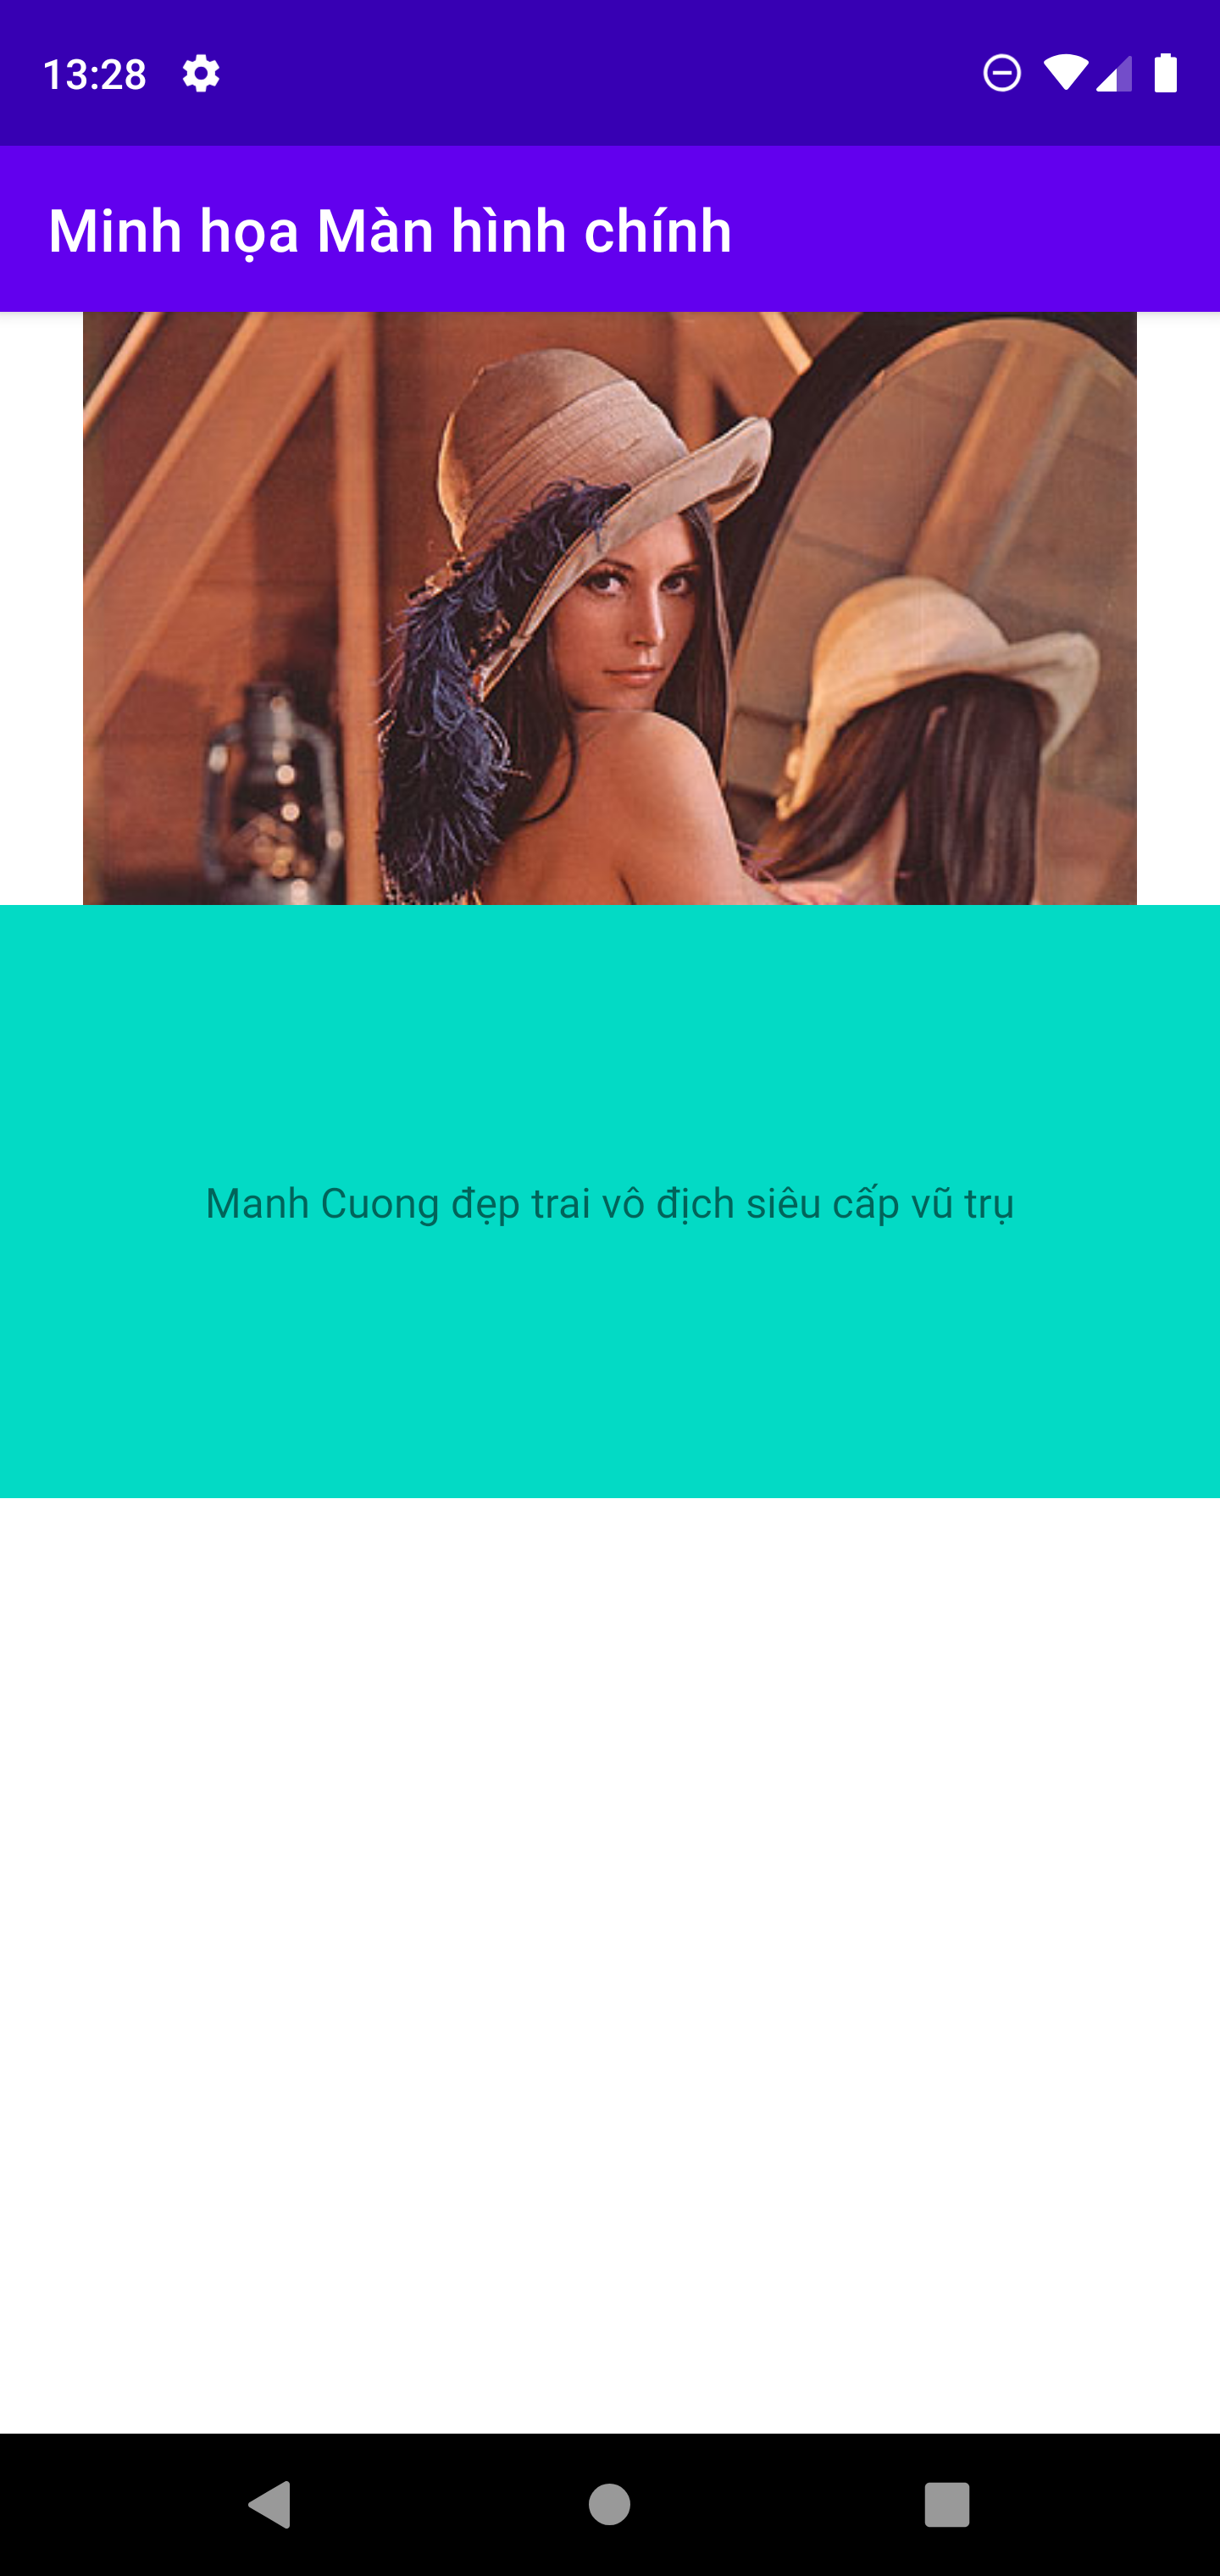
\includegraphics[height=0.7\textheight]{images/10.png}
            \caption{\centering\tiny{Hình 14: Minh họa màn hình chính của ứng dụng}}
        \end{figure}
        \column{0.7\linewidth}
        \indent \textbf{\texttt{HomeModel.java}}
        \begin{figure}
            \centering
            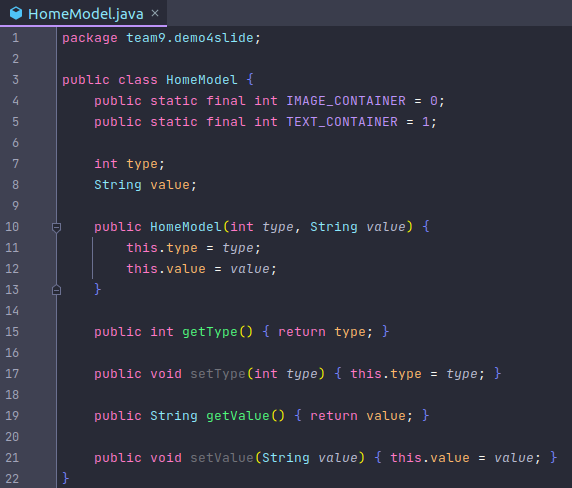
\includegraphics[width=\textwidth]{images/17.png}
        \end{figure}
    \end{columns}
\end{frame}

\begin{frame}
    \begin{columns}
        \column{0.3\linewidth}
        \begin{figure}
            \centering
            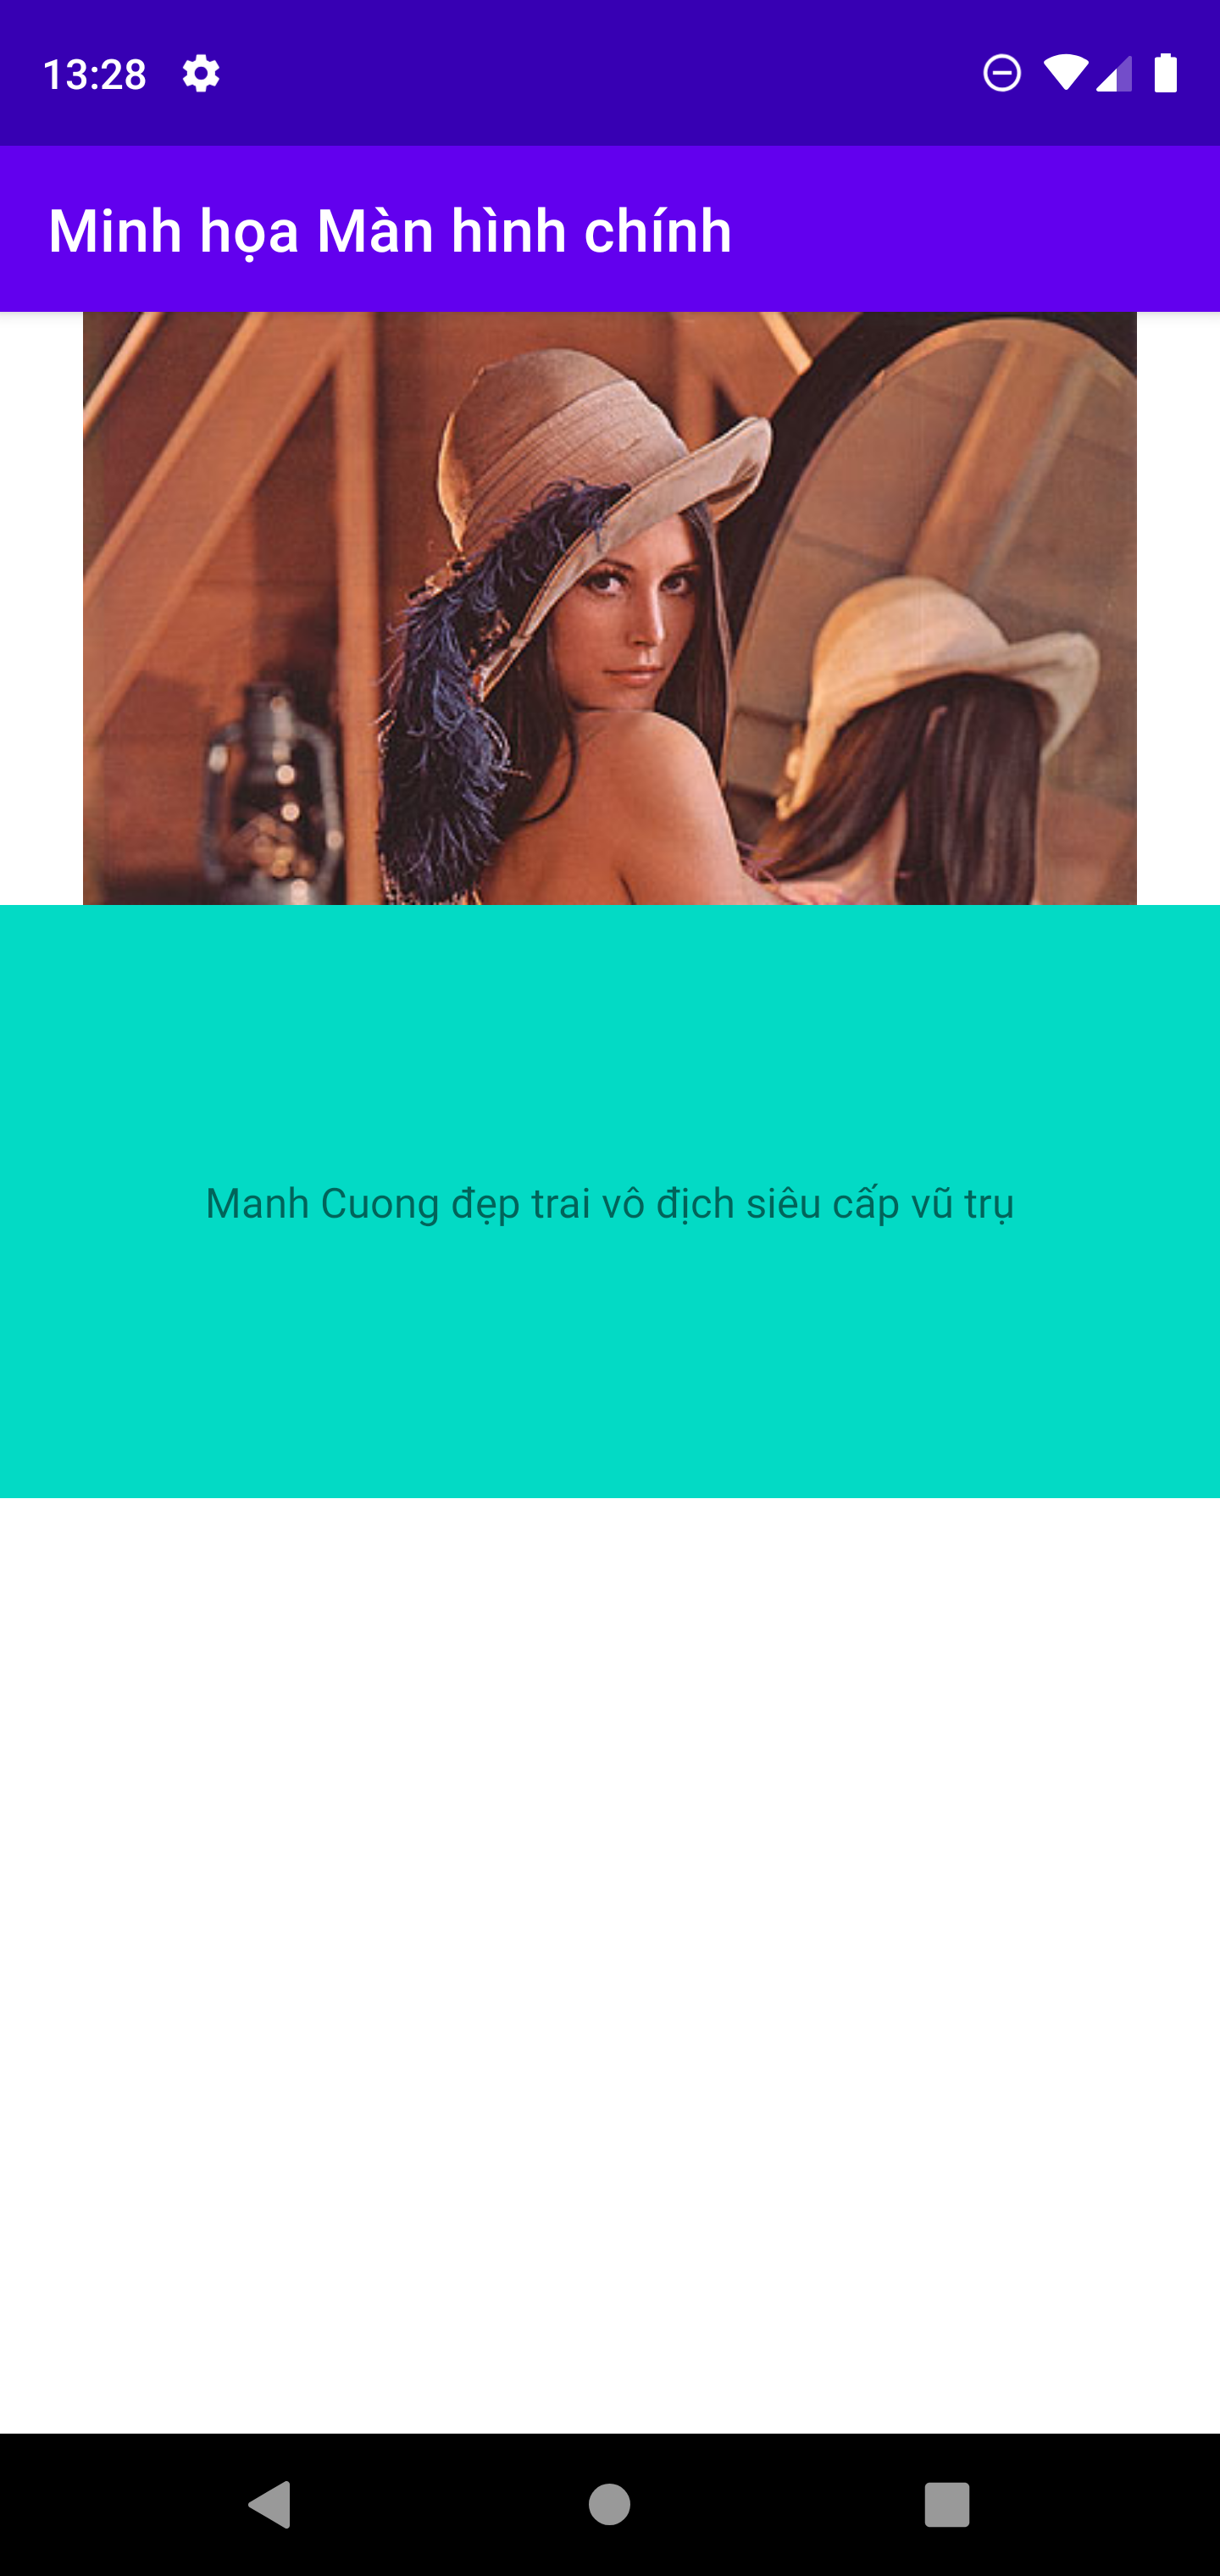
\includegraphics[height=0.7\textheight]{images/10.png}
            \caption{\centering\tiny{Hình 14: Minh họa màn hình chính của ứng dụng}}
        \end{figure}
        \column{0.7\linewidth}
        \indent \textbf{\texttt{HomeAdapter.java}} (1)
        \begin{figure}
            \centering
            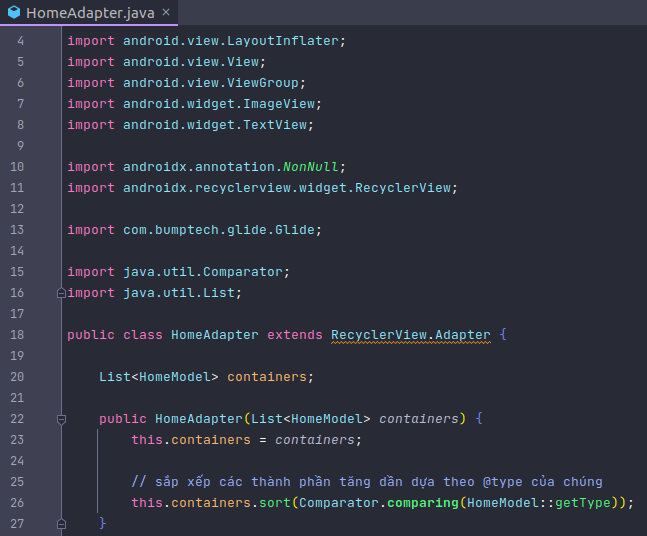
\includegraphics[width=\textwidth]{images/18.png}
        \end{figure}
    \end{columns}
\end{frame}

\begin{frame}
    \begin{columns}
        \column{0.3\linewidth}
        \begin{figure}
            \centering
            \includegraphics[height=0.7\textheight]{images/10.png}
            \caption{\centering\tiny{Hình 14: Minh họa màn hình chính của ứng dụng}}
        \end{figure}
        \column{0.7\linewidth}
        \indent \textbf{\texttt{HomeAdapter.java}} (2)
        \begin{figure}
            \centering
            \includegraphics[width=\textwidth]{images/19.png}
        \end{figure}
    \end{columns}
\end{frame}

\begin{frame}
    \begin{columns}
        \column{0.3\linewidth}
        \begin{figure}
            \centering
            \includegraphics[height=0.7\textheight]{images/10.png}
            \caption{\centering\tiny{Hình 14: Minh họa màn hình chính của ứng dụng}}
        \end{figure}
        \column{0.7\linewidth}
        \indent \textbf{\texttt{HomeAdapter.java}} (3)
        \begin{figure}
            \centering
            \includegraphics[width=\textwidth]{images/20.png}
        \end{figure}
    \end{columns}
\end{frame}

\begin{frame}
    \begin{columns}
        \column{0.3\linewidth}
        \begin{figure}
            \centering
            \includegraphics[height=0.7\textheight]{images/10.png}
            \caption{\centering\tiny{Hình 14: Minh họa màn hình chính của ứng dụng}}
        \end{figure}
        \column{0.7\linewidth}
        \indent \textbf{\texttt{HomeAdapter.java}} (4)
        \begin{figure}
            \centering
            \includegraphics[width=\textwidth]{images/21.png}
        \end{figure}
    \end{columns}
\end{frame}

\begin{frame}
    \begin{columns}
        \column{0.3\linewidth}
        \begin{figure}
            \centering
            \includegraphics[height=0.7\textheight]{images/10.png}
            \caption{\centering\tiny{Hình 14: Minh họa màn hình chính của ứng dụng}}
        \end{figure}
        \column{0.7\linewidth}
        \indent \textbf{\texttt{HomeActivity.java}} (1)
        \begin{figure}
            \centering
            \includegraphics[width=\textwidth]{images/22.png}
        \end{figure}
    \end{columns}
\end{frame}

\begin{frame}
    \begin{columns}
        \column{0.3\linewidth}
        \begin{figure}
            \centering
            \includegraphics[height=0.7\textheight]{images/10.png}
            \caption{\centering\tiny{Hình 14: Minh họa màn hình chính của ứng dụng}}
        \end{figure}
        \column{0.7\linewidth}
        \indent \textbf{\texttt{HomeActivity.java}} (2)
        \begin{figure}
            \centering
            \includegraphics[width=\textwidth]{images/23.png}
        \end{figure}
    \end{columns}
\end{frame}

\begin{frame}
    \frametitle{Các màn hình và chức năng kèm theo (8)}
    \framesubtitle{Chức năng tìm kiếm}

    \begin{columns}
        \column{0.3\linewidth}
        \begin{figure}
            \centering
            \includegraphics[height=0.7\textheight]{images/09.png}
            \caption{\centering\tiny{Hình 15: Chức năng tìm kiếm sản phẩm}}

        \end{figure}
        \column{0.7\linewidth}
        \indent \textbf{Các thành phần và chức năng kèm theo trên màn hình:}
        \begin{itemize}
            \item Khi người dùng nhấn vào bất kì một menu item search nào, một search box như hình trên sẽ hiển thị ra, đồng thời người dùng sẽ được đưa đến một fragment khác, nơi các sản phẩm được tìm kiểm sẽ hiển thị dưới dạng một GridView.
            \item Ở đây, nhóm tìm kiếm các sản phẩm dựa vào ba từ khóa là \textsf{\color{teal} dress}, \textsf{\color{teal} isola} và \textsf{\color{teal} hồi}, thì toàn bộ các sản phẩm được tìm ra bên dưới đều có tên chứa ít nhất một từ mà người dùng nhập vào.
        \end{itemize}
    \end{columns}
\end{frame}

\begin{frame}
    \frametitle{Các màn hình và chức năng kèm theo (9)}
    \framesubtitle{Chức năng tìm kiếm - Mã nguồn minh họa}

    \begin{columns}
        \column{0.3\linewidth}
        \begin{figure}
            \centering
            \includegraphics[height=0.7\textheight]{images/40.png}
            \caption{\centering\tiny{Hình 16: Minh họa chức năng tìm kiếm sản phẩm}}
        \end{figure}
        \column{0.7\linewidth}
        \indent Cấu trúc cây thư mục:
        \begin{figure}
            \centering
            \includegraphics[height=0.68\textheight]{images/41.png}
        \end{figure}
    \end{columns}
\end{frame}

\begin{frame}
    \begin{columns}
        \column{0.3\linewidth}
        \begin{figure}
            \centering
            \includegraphics[height=0.7\textheight]{images/40.png}
            \caption{\centering\tiny{Hình 16: Minh họa chức năng tìm kiếm sản phẩm}}
        \end{figure}
        \column{0.7\linewidth}
        \indent \texttt{AndroidManifest.xml}
        \begin{figure}
            \centering
            \includegraphics[width=\textwidth]{images/42.png}
        \end{figure}
    \end{columns}
\end{frame}

\begin{frame}
    \begin{columns}
        \column{0.3\linewidth}
        \begin{figure}
            \centering
            \includegraphics[height=0.7\textheight]{images/40.png}
            \caption{\centering\tiny{Hình 16: Minh họa chức năng tìm kiếm sản phẩm}}
        \end{figure}
        \column{0.7\linewidth}
        \indent \texttt{build.gradle}
        \begin{figure}
            \centering
            \includegraphics[width=\textwidth]{images/43.png}
        \end{figure}
    \end{columns}
\end{frame}

\begin{frame}
    \begin{columns}
        \column{0.3\linewidth}
        \begin{figure}
            \centering
            \includegraphics[height=0.7\textheight]{images/40.png}
            \caption{\centering\tiny{Hình 16: Minh họa chức năng tìm kiếm sản phẩm}}
        \end{figure}
        \column{0.7\linewidth}
        \indent \texttt{activity\_search.xml}
        \begin{figure}
            \centering
            \includegraphics[width=\textwidth]{images/44.png}
        \end{figure}
    \end{columns}
\end{frame}

\begin{frame}
    \begin{columns}
        \column{0.3\linewidth}
        \begin{figure}
            \centering
            \includegraphics[height=0.7\textheight]{images/40.png}
            \caption{\centering\tiny{Hình 16: Minh họa chức năng tìm kiếm sản phẩm}}
        \end{figure}
        \column{0.7\linewidth}
        \indent \texttt{item\_search.xml}
        \begin{figure}
            \centering
            \includegraphics[width=\textwidth]{images/45.png}
        \end{figure}
    \end{columns}
\end{frame}

\begin{frame}
    \begin{columns}
        \column{0.3\linewidth}
        \begin{figure}
            \centering
            \includegraphics[height=0.7\textheight]{images/40.png}
            \caption{\centering\tiny{Hình 16: Minh họa chức năng tìm kiếm sản phẩm}}
        \end{figure}
        \column{0.7\linewidth}
        \indent \texttt{SongModel.java}
        \begin{figure}
            \centering
            \includegraphics[width=\textwidth]{images/46.png}
        \end{figure}
    \end{columns}
\end{frame}


\begin{frame}
    \begin{columns}
        \column{0.3\linewidth}
        \begin{figure}
            \centering
            \includegraphics[height=0.7\textheight]{images/40.png}
            \caption{\centering\tiny{Hình 16: Minh họa chức năng tìm kiếm sản phẩm}}
        \end{figure}
        \column{0.7\linewidth}
        \indent \texttt{SongModel} trong Firestore
        \begin{figure}
            \centering
            \includegraphics[width=\textwidth]{images/47.png}
        \end{figure}
    \end{columns}
\end{frame}

\begin{frame}
    \begin{columns}
        \column{0.3\linewidth}
        \begin{figure}
            \centering
            \includegraphics[height=0.7\textheight]{images/40.png}
            \caption{\centering\tiny{Hình 16: Minh họa chức năng tìm kiếm sản phẩm}}
        \end{figure}
        \column{0.7\linewidth}
        \indent \texttt{SearchAdapter.java} (1)
        \begin{figure}
            \centering
            \includegraphics[width=\textwidth]{images/48.png}
        \end{figure}
    \end{columns}
\end{frame}

\begin{frame}
    \begin{columns}
        \column{0.3\linewidth}
        \begin{figure}
            \centering
            \includegraphics[height=0.7\textheight]{images/40.png}
            \caption{\centering\tiny{Hình 16: Minh họa chức năng tìm kiếm sản phẩm}}
        \end{figure}
        \column{0.7\linewidth}
        \indent \texttt{SearchAdapter.java} (2)
        \begin{figure}
            \centering
            \includegraphics[width=\textwidth]{images/49.png}
        \end{figure}
    \end{columns}
\end{frame}

\begin{frame}
    \begin{columns}
        \column{0.3\linewidth}
        \begin{figure}
            \centering
            \includegraphics[height=0.7\textheight]{images/40.png}
            \caption{\centering\tiny{Hình 16: Minh họa chức năng tìm kiếm sản phẩm}}
        \end{figure}
        \column{0.7\linewidth}
        \indent \texttt{SearchActivity.java} (1)
        \begin{figure}
            \centering
            \includegraphics[width=\textwidth]{images/50.png}
        \end{figure}
    \end{columns}
\end{frame}

\begin{frame}
    \begin{columns}
        \column{0.3\linewidth}
        \begin{figure}
            \centering
            \includegraphics[height=0.7\textheight]{images/40.png}
            \caption{\centering\tiny{Hình 16: Minh họa chức năng tìm kiếm sản phẩm}}
        \end{figure}
        \column{0.7\linewidth}
        \indent \texttt{SearchActivity.java} (2)
        \begin{figure}
            \centering
            \includegraphics[width=\textwidth]{images/51.png}
        \end{figure}
    \end{columns}
\end{frame}

\begin{frame}
    \frametitle{Chạy thử ứng dụng}
    \begin{center}
        \Large{Link Youtube: \href{https://youtu.be/yRglZ4Segkk}{\color{blue} https://youtu.be/yRglZ4Segkk}}\\
        ~\\
        ~\\
        \includegraphics[width=0.6\textwidth]{images/demo.png}
    \end{center}
\end{frame}

\begin{frame}
    \frametitle{Tài nguyên và tham khảo}
    \begin{itemize}
        \item Logo ứng dụng và tên Clover: được nhóm xin phép từ nhãn hàng Clover và đã được sự đồng ý từ chị chủ nhãn hàng, trang bán hàng của nhãn hàng tại \href{https://www.facebook.com/TiemmaynhaAn}{\color{blue} https://www.facebook.com/TiemmaynhaAn}.
        \item Về hình ảnh người mẫu Việt Nam ở mục sản phẩm mới: là bạn Phan Hữu Lộc - cựu sinh viên K17 khoa Sinh học của trường Đại Học Khoa Học Tự Nhiên TP.HCM và là người mẫu của nhãn hàng Clover phía trên.
        \item Các hình ảnh sản phẩm khác được nhóm lấy về (chưa xin phép) từ trang bán hàng Farfetch tại \href{https://www.farfetch.com}{\color{blue} https://www.farfetch.com}.
        \item Về các kĩ thuật code trong đồ án ngoài slide của Thầy lý thuyết nhóm còn tham khảo thêm trong cuốn \textbf{\color{teal} Android Programming for Beginners}, link sách tại \href{https://www.amazon.com/Android-Programming-Beginners-depth-full-featured/dp/1800563434}{\color{blue} https://www.amazon.com/Android-Programming-Beginners-depth-full-featured/dp/1800563434}.
    \end{itemize}
\end{frame}

\begin{frame}
    \frametitle{Hỏi đáp và kết thúc}
    \includegraphics[width=\textwidth]{images/ask_and_answer.jpg}
\end{frame}

\begin{frame}
    \Huge{\centerline{HẾT}}
    \Large{\centerline{Cảm ơn Thầy và các bạn đã chú ý lắng nghe.}}
\end{frame}

%----------------------------------------------------------------------------------------

\end{document}